\begin{figure}[!h]
\begin{center}
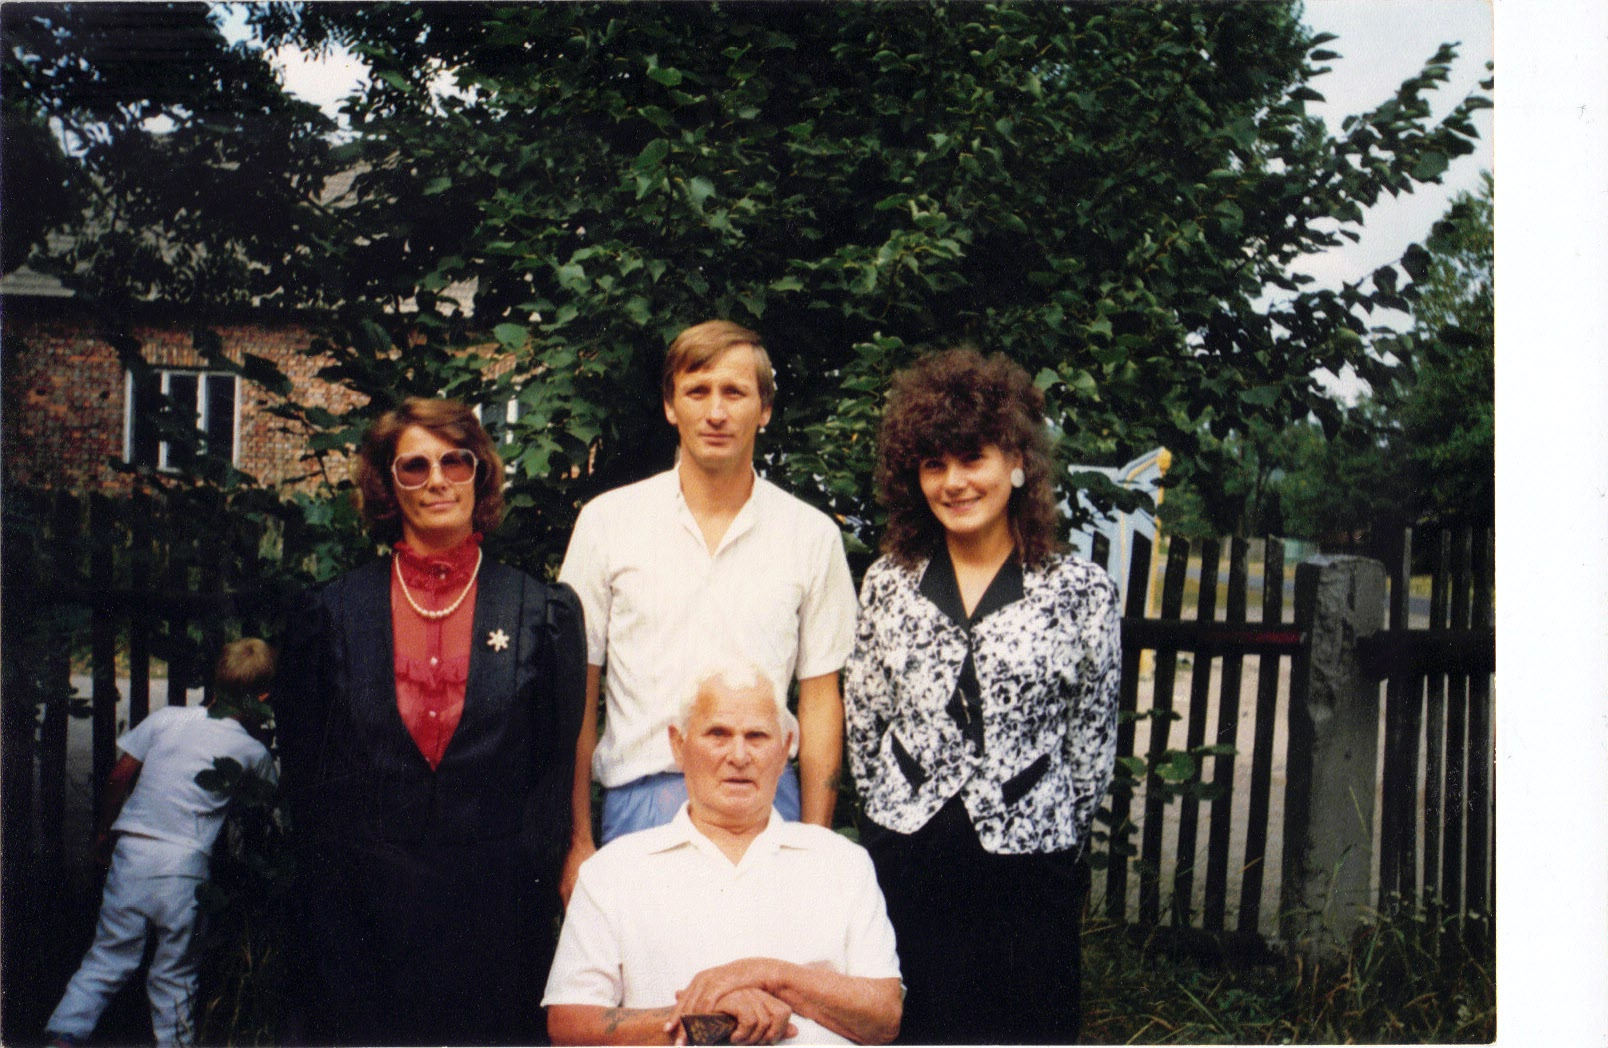
\includegraphics[width=0.7\textwidth]{zdjecia/franciszek_glab_z_dziecmi.jpg}
\caption[Franciszek Głąb z dziećmi]{Franciszek Głąb z dziećmi, od lewej: Czesławą Świerczyńską, Mirosławem Głąbem i Mirosławą Jabłońską}
\label{rys:franciszek_glab_z_dziecmi}
\end{center}
\end{figure}

Ojciec Czesławy, a wasz dziadek Franciszek jako się rzekło, wywodzi się z płodnego rodu Walentego i Antoniny Głąbów. Oto jak ten fakt został zapisany w księdze ślubów Parafii Włodowice (tłumaczę z rosyjskiego): Wydarzyło się w Parafii Włodowice trzydziestego pierwszego sierpnia (wg kalendarza juliańskiego), dwunastego września (wg kalendarza gregoriańskiego, tj. naszego) 1894 roku o dwunastej w południe. Oświadczamy, że w obecności świadków: Karola Haładusa pięćdziesiąt lat i Antoniego Łyszczarza pięćdziesiąt sześć lat, obydwóch włościan, rolników, mieszkańców wsi Góra, zawarty został tego dnia religijny związek małżeński między Walentym Głąbem – młodzianem, dwadzieścia pięć lat, urodzonym i mieszkającym przy rodzicach we wsi Mirów, Parafii Niegowa, synem Macieja i Marianny z domu Hamerla, małżonków Głąb i Antoniną Łyszczarz, panną dziewiętnastoletnią pozostającą i mieszkającą przy opiekunie Kasprze Łyszczarzu we wsi Góra, parafii Włodowice, córką już zmarłych małżonków Macieja i jego żony Józefy z domu Boniek, małżonków Łyszczarz. Małżeństwo to zostało poprzedzone trzykrotnymi zapowiedziami wygłoszonymi w parafii Włodowice i Niegowa (dalej podane są daty tych ogłoszeń oraz fakt, że ów akt ślubu został zaślubionym i świadkom odczytany, ale przez nas tylko podpisany ponieważ zaślubieni i świadkowie pisać nie umieją. Ten akt ślubu jest jedyną informacją o roku urodzin prababki Antoniny Łyszczarz ponieważ księga urodzeń za lata 1865 do września 1875 Parafii Włodowice zaginęła. Dokładną datę jej urodzenia znajdujemy w akcie jej zgonu. Urodziła się 18 VI 1875 r. w Górze Włodowskiej. Zdjęcie aktu ślubu Walentego Głąba z Antoniną Łyszczarz prezentujemy na 1 str. naszej historii (ryc.~\ref{rys:akt_slubu_walentego_glaba_i_antoniny_lyszczarz}).

Natomiast zachował się akt ślubu jej rodziców, którego tłumaczenie z rosyjskiego tutaj przytaczam: Wydarzyło się w Parafii Włodowice trzeciego (wg kalend. Juliańskiego), piętnastego czerwca 1874 r. (zatem Antonina była ich pierwszym dzieckiem i urodziła się najpewniej w 1875 r., bowiem gdyby się urodziła w 1876 r. i później byłaby zapisana w istniejącej do dziś księdze urodzeń) o dziewiątej rano. Oświadczamy, że w obecności świadków Andrzeja Bomby -- trzydzieści lat i Ignacego Filipka (być może Filipeckiego -- trudno odczytać) sześćdziesiąt lat, obaj kamienicznicy (albo gospodarze) z Włodowic zawarty został tego dnia religijny małżeński związek między Maciejem Łyszczarzem, kawalerem dwudziestoośmioletnim urodzonym w Górze z Bartłomieja i Ewy (z Filipeckich) oboje zmarłych, żołnierzem w stanie spoczynku pod numerem sto trzy w Górze mieszkającym z Józefą Boniek, panną dwudziestoletnią urodzoną we Włodowicach z Pawła i Zofii, oboje zmarłych, u siostry we Włodowicach mieszkającą. Małżeństwo to poprzedziły zapowiedzi. Zatem rodzice Antoniny także byli, i to oboje, sierotami! Co za trudny los prababki Antoniny! A ponadto ksiądz sporządzający ów akt miał widać lekceważący stosunek do sierot, skoro nie podaje nazwiska matki kawalera ani też panny...

\begin{figure}[!h]
\begin{center}
\includegraphics[width=0.8\textwidth]{zdjecia/akt_slubu_jozefa_lyszczarza_i_jozefy_boniek.jpg}
\caption[Akt ślubu Macieja Łyszczarza z Józefą Boniek]{Akt ślubu Macieja Łyszczarza z Józefą Boniek}
\label{rys:akt_slubu_jozefa_lyszczarza_i_jozefy_boniek}
\end{center}
\end{figure}

Że matka pana młodego -- Macieja Łyszczarza wywodziła się z Filipeckich wiemy z jego aktu urodzenia, który tutaj przytaczamy: ,,Działo się w mieście Włodowicach dnia 15 II 1845 r. Stawił sie oto Bartłomiej Łyszczarz , zagrodnik lat 24 mający we wsi Górze zamieszkały w obecności Piotra Filipeckiego, lat 26 i Marcina Mygi, lat 50, obydwóch zagrodników we wsi Górze zamieszkałych i okazał nam dziecię płci męskiej urodzone we wsi Górze dnia dzisiejszego w domu pod numerem 10 z jego małżonki Ewy z Filipeckich lat 30 mającej. Dziecięciu temu na Chrzcie św. odbytym w dniu dzisiejszym nadane zostało imię Maciey, a rodzicami jego chrzestnymi byli wyżej wspomniany Piotr Filipecki z Antoniną Samkową.''

%TODO *** Tu zdj. aktu urodz. Macieja Łyszczarza, zdj. nr 239 w pliku Archiwum diecezj.}

Postanowiłem dokładniej spojrzeć na los babki Antoniny Łyszczarz, ponieważ wchodziła w związek małżeński z Walentym Głąbem jako zupełna sierota! Chciałem uzyskać odpowiedź na kilka pytań: 1. Ile lat miała Antonina Łyszczarz, gdy utraciła rodziców? 2. Kim był dla niej Kasper Łyszczarz – jej urzędowy opiekun podczas jej zaślubin z Walentym Głąbem? 3. Kiedy pobrali się jej rodzice? Jej rodzice również byli zupełnymi sierotami, gdy się pobierali. Cytuję za księgą ślubów: ,,Działo się 15 VI 1874 r. w obecności świadków: Andrzeja Bomby (30 lat) i Ignacego Filipskiego (60 lat), obydwóch ,,domowładielcew'' z Włodowic zawarto tego czasu religijny związek małżeński między Maciejem Łyszczarzem -- kawalerem -- 28 lat, urodzonym w Górze z Bartłomieja i Ewy -- zmarłych -- ,,otstawnoj sołdat za nomierom sto tri'' w Górze zamieszkałym – z Józefą Boniek – panną 20 lat, urodzoną we Włodowicach z Pawła i Zofii -- zmarłych, u siostry (Marianny lub Agaty) mieszkająca.

Odpowiedź na pierwsze pytanie ukazuje bezmiar cierpień, jakie musiały stać się udziałem małej Antosi Łyszczarzównej. Ojca Macieja pewnie w ogóle nie znała, gdyż jako żołnierz armii carskiej wkrótce po ślubie ,,paszoł w sołdaty''. Kto wie czy było dane Maciejowi obaczyć swe jedyne dziecię? Tymczasem jego małżonka Józefa złakniona od wielu miesięcy mężczyzny pozwoliła sobie na flirt, którego owocem był Hilary Łyszczarz urodzony 16 II 1879 r. w Górze, o czym księdza powiadomiła Zofia Dyrdoń -- ,,powiwalnaja babka'' z Kotowic, czyli ówczesna akuszerka w obecności świadków Jana Białego (25 lat) i Jana Chwalby (40 lat), rolników z Góry, oświadczając, że to dziecię urodziło się o północy z Józefy Łyszczarz (26 lat) i ,,nieizwiestnago ot'ca''. Temu dziecięciu przy chrzcie św. nadano imię Hilary, a chrzestnymi byli Jan Biały i Marianna Chwalba (ryc.~\ref{rys:akt_urodzenia_hilarego_lyszczarza}).


\begin{figure}[!h]
\begin{center}
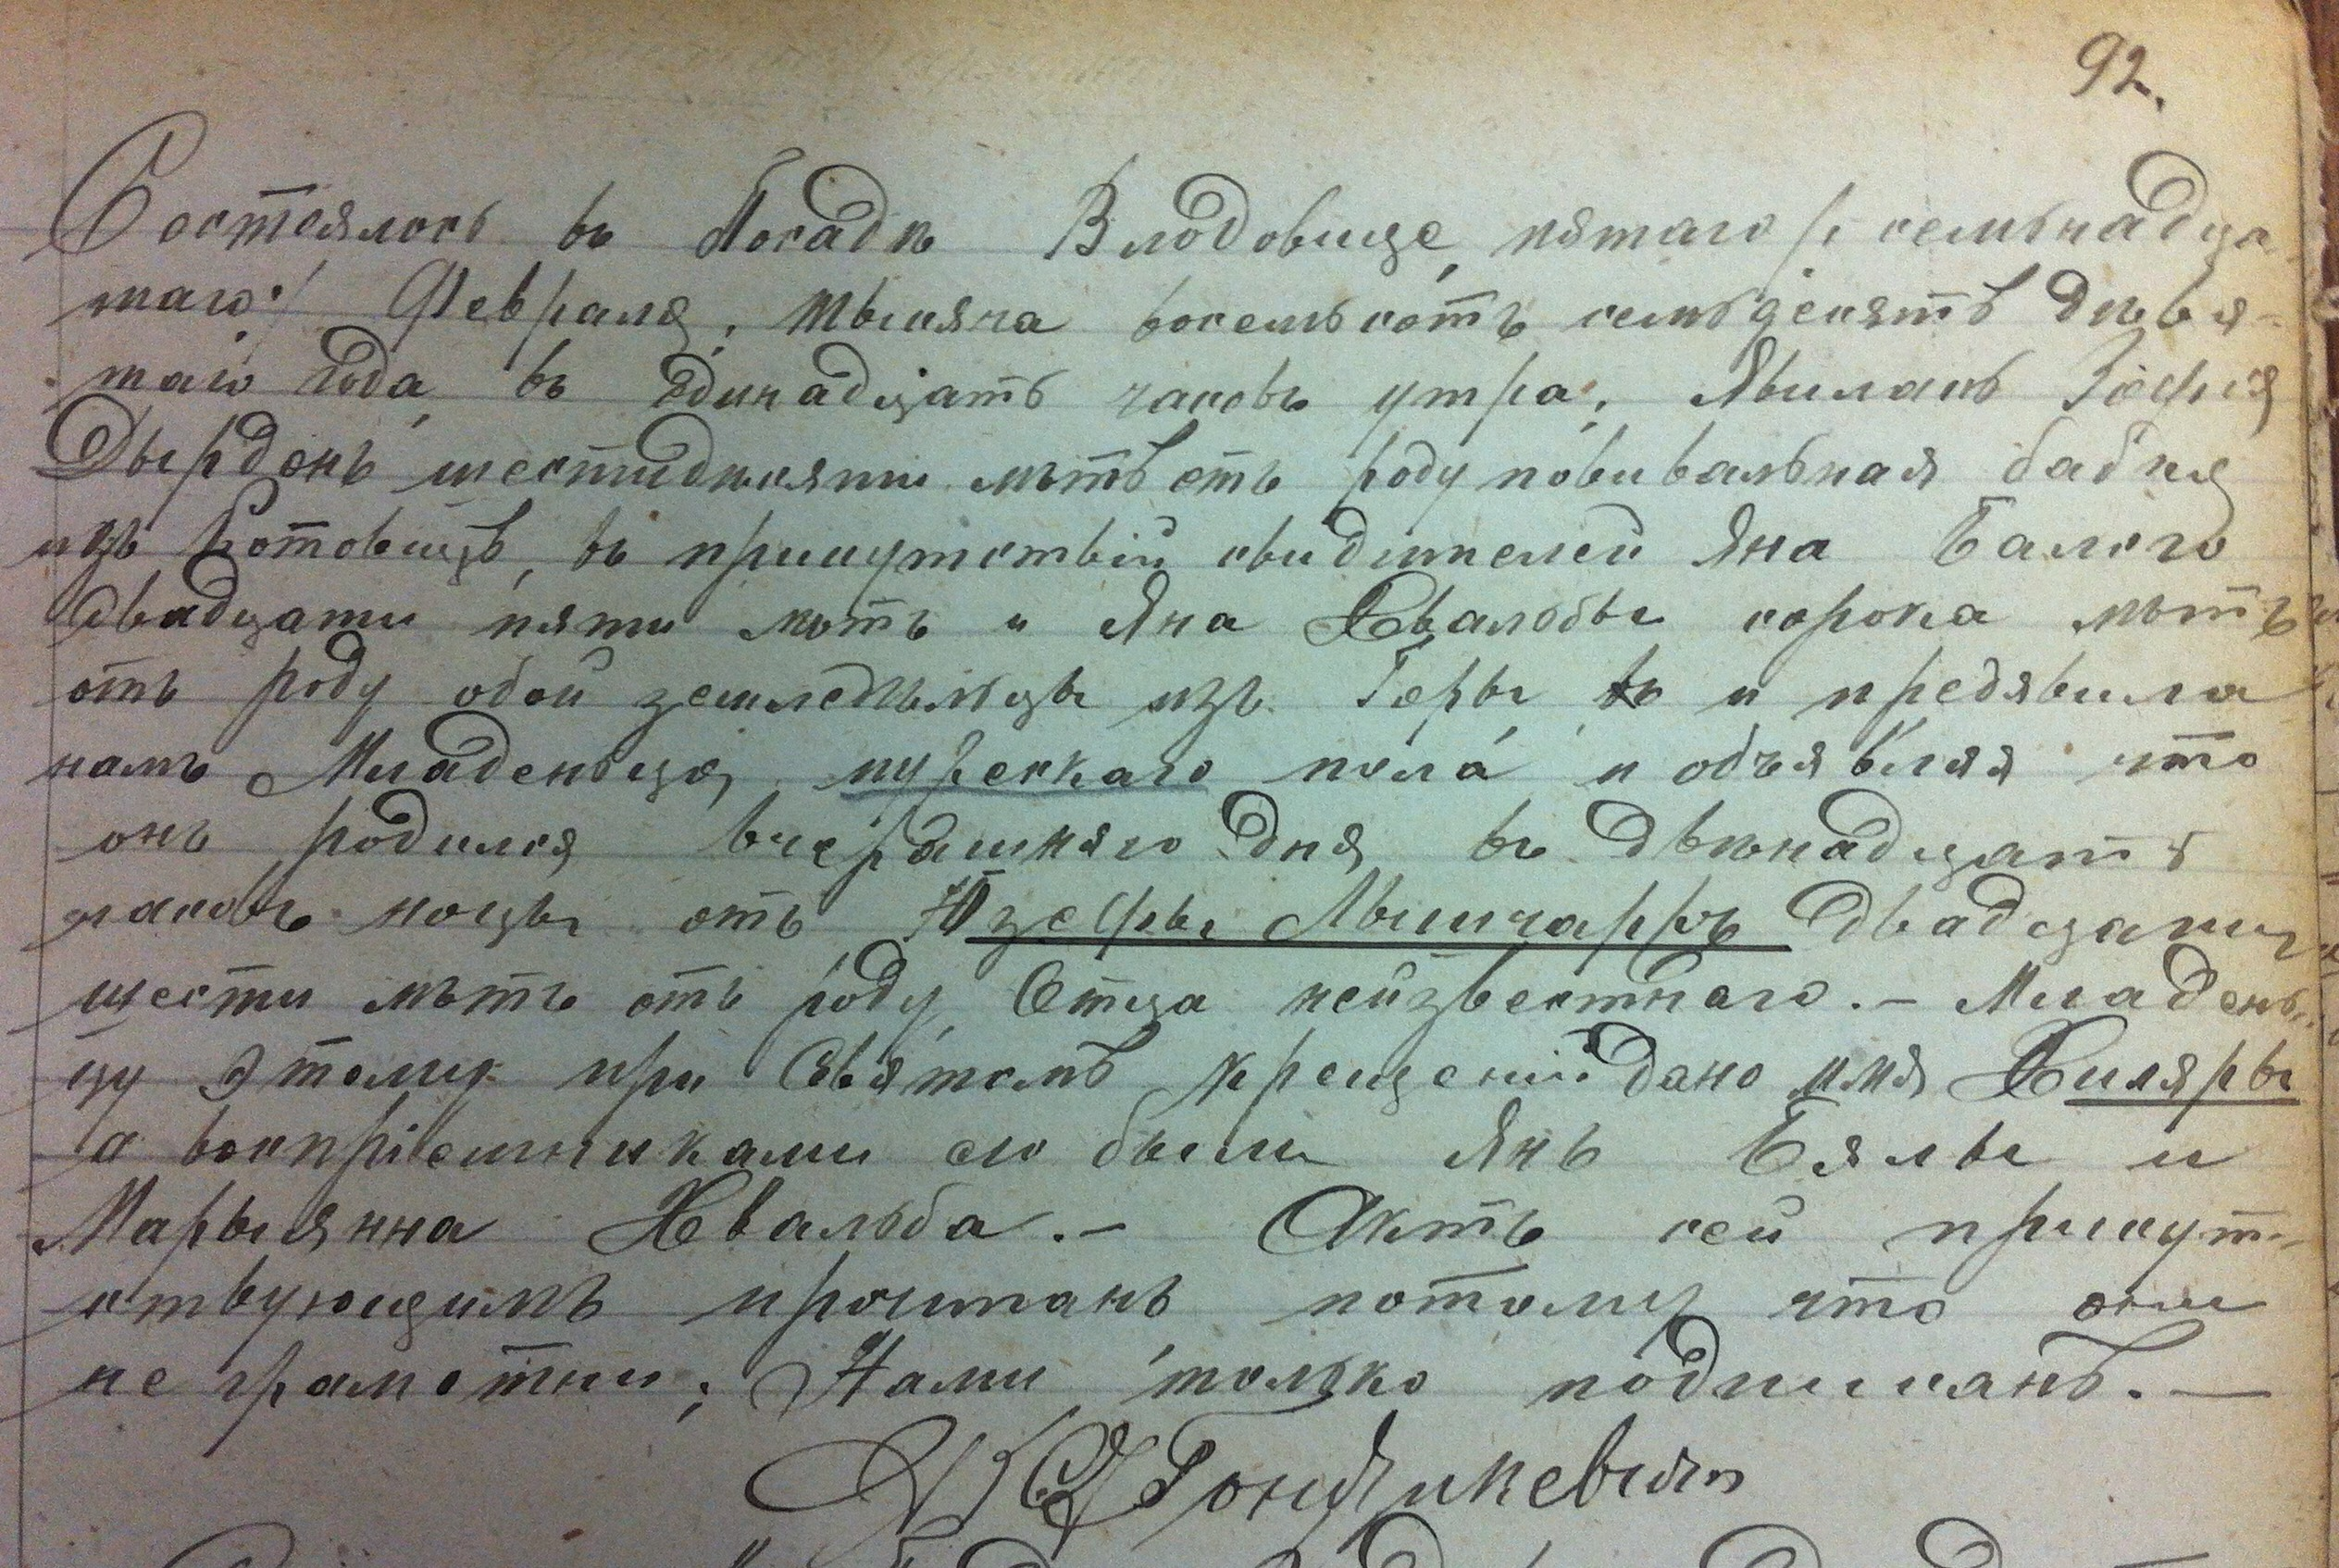
\includegraphics[width=0.75\textwidth]{zdjecia/akt_urodzenia_hilarego_lyszczarza.jpg}
\caption[Akt urodzenia Hilarego Łyszczarza]{Akt urodzenia Hilarego Łyszczarza -- brata Antoniny Głąb z domu Łyszczarz}
\label{rys:akt_urodzenia_hilarego_lyszczarza}
\end{center}
\end{figure}

Tenże Hilary w wieku 26 lat ożenił się 14 lutego 1906 r. w Niegowie z Marianną Szczepańczyk (23 lata), córką zmarłego Marcina Szczepańczyka i żyjącej wdowy po nim - Franciszki z domu Sławek (ryc.~\ref{rys:akt_slubu_marianny_i_hilarego_lyszczarzow}).

\begin{figure}[!h]
\begin{center}
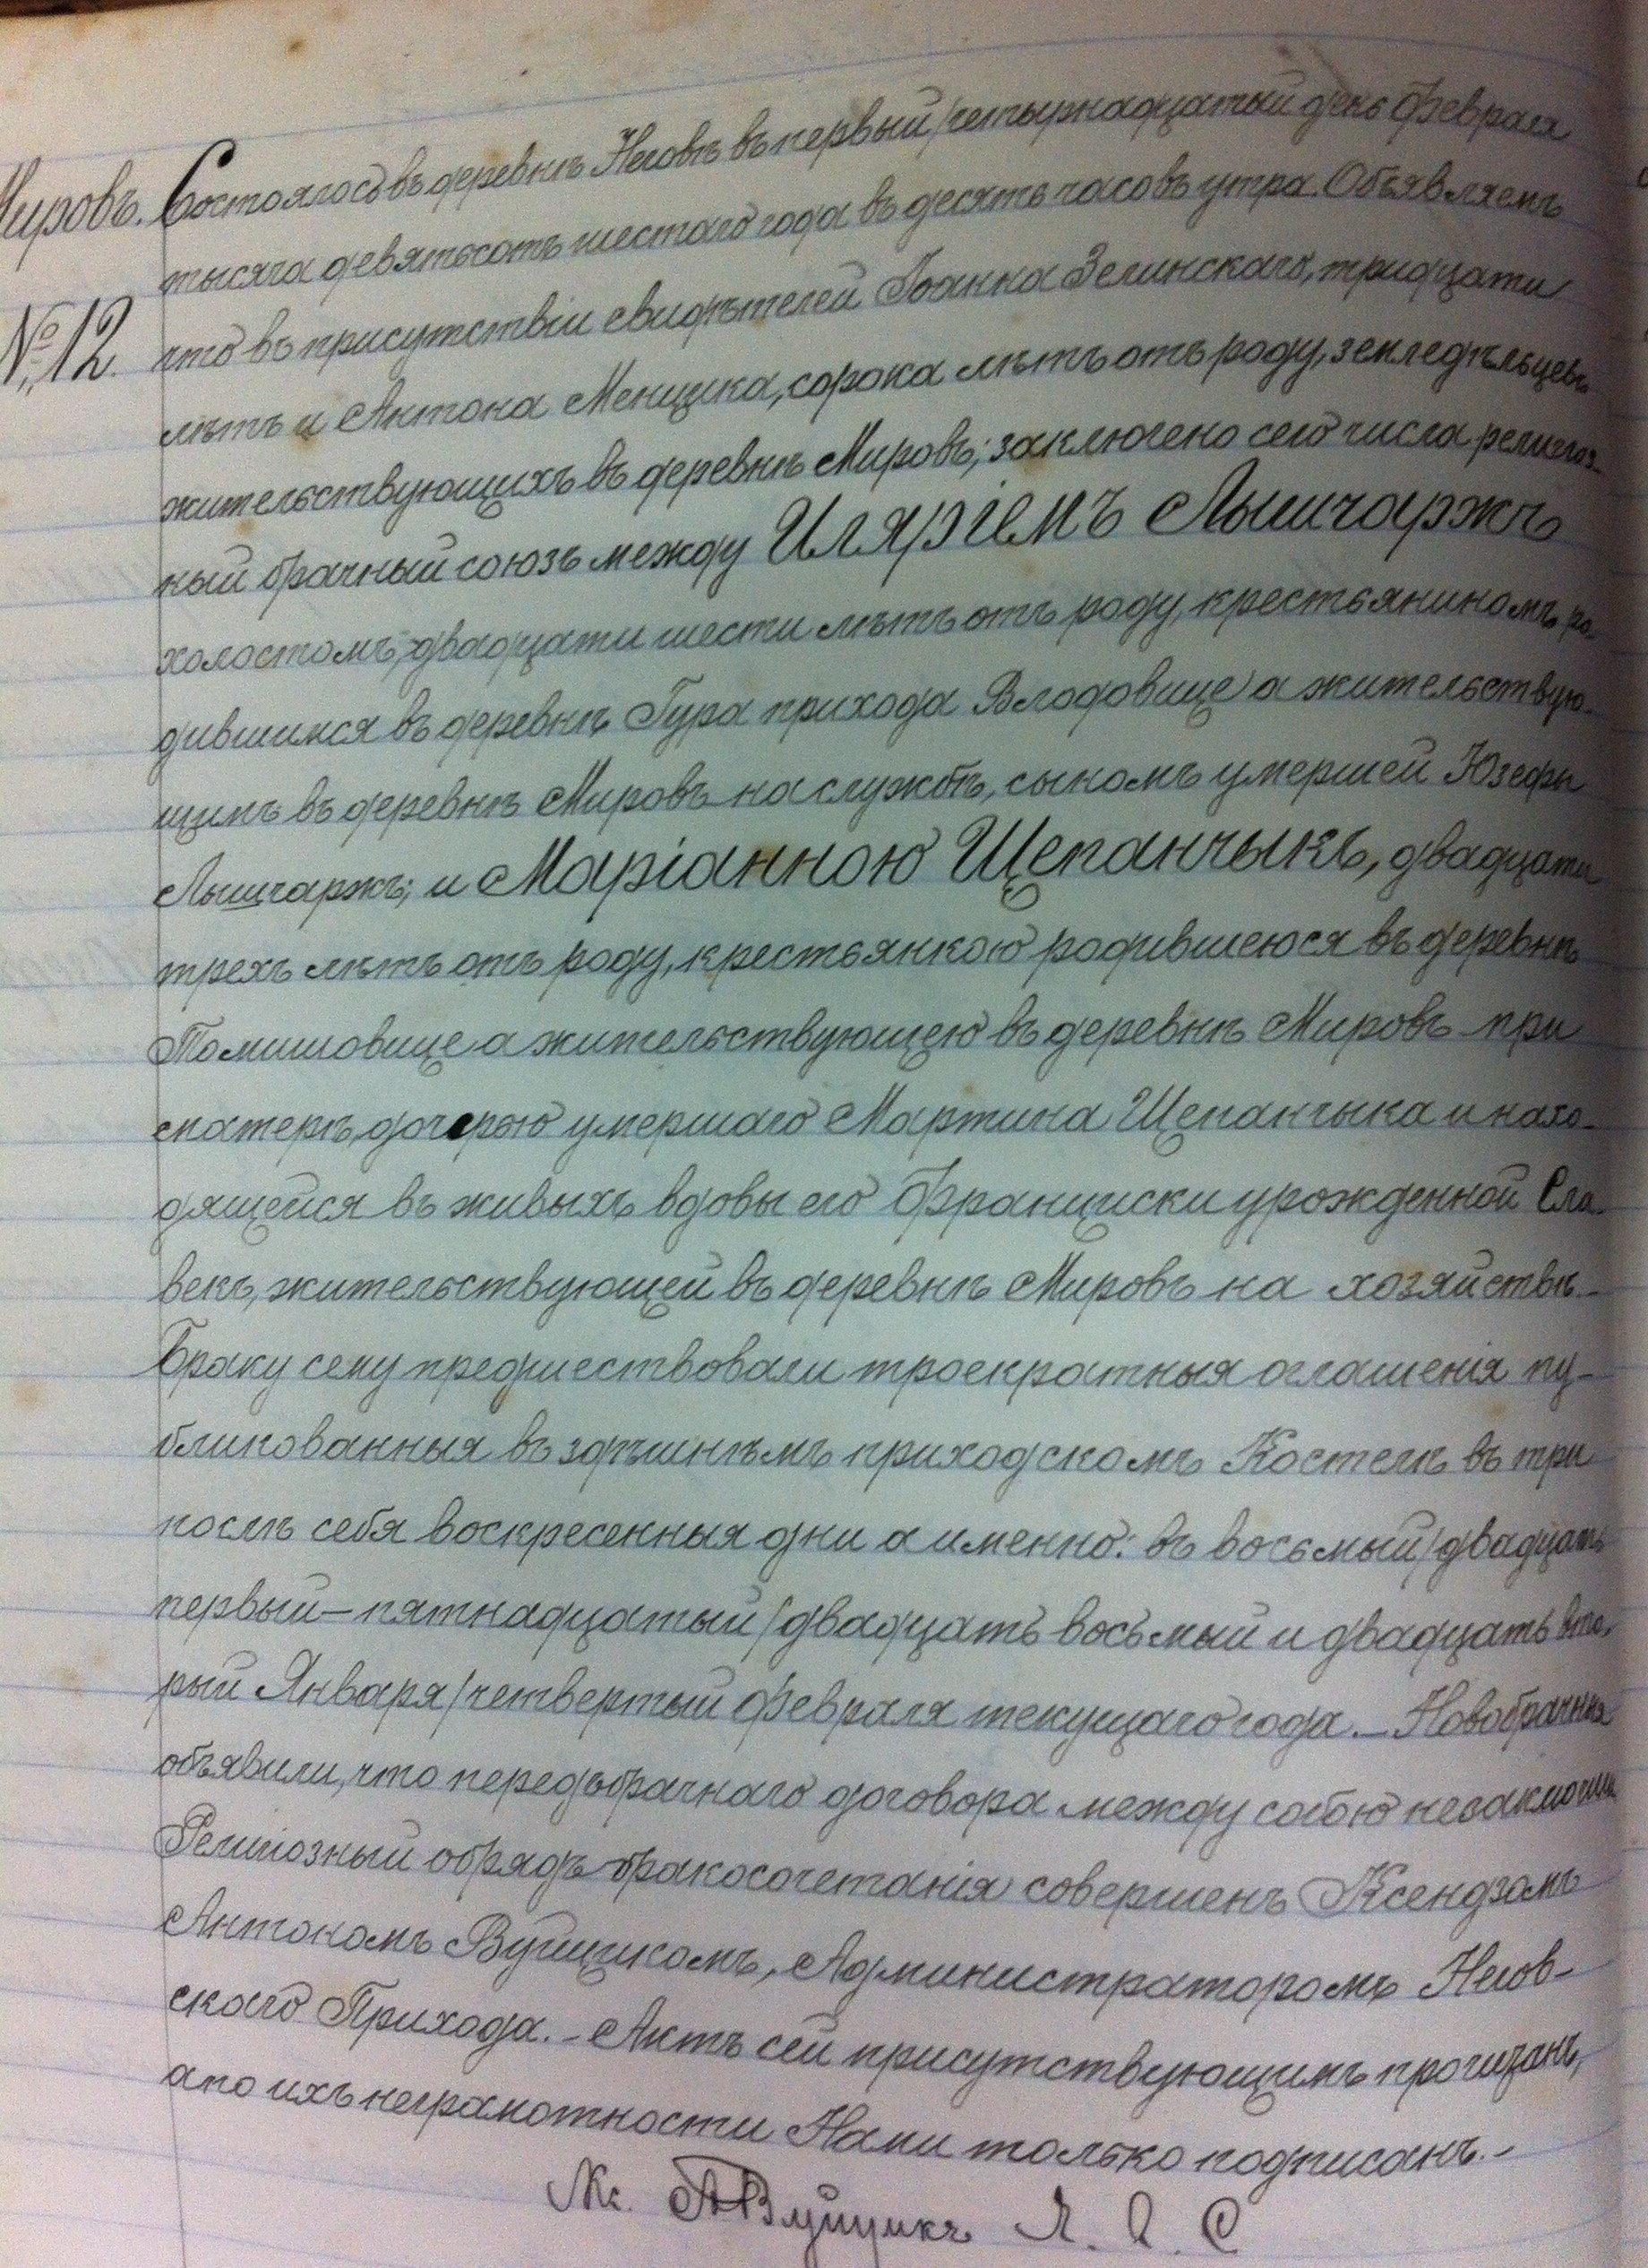
\includegraphics[width=0.5\textwidth]{zdjecia/akt_slubu_marianny_i_hilarego_lyszczarzow.jpg}
\caption[Akt ślubu Hilarego Łyszczarza z Marianną Szczepańczyk]{Akt ślubu Hilarego Łyszczarza, brata Antoniny Głąb z domu Łyszczarz, z Marianną Szczepańczyk}
\label{rys:akt_slubu_marianny_i_hilarego_lyszczarzow}
\end{center}
\end{figure}

Panna Młoda urodziła się w Tomiszowicach, ale mieszkała w Mirowie na gospodarstwie przy swojej matce. Można więc przypuszczać, że Hilary do tej pory mieszkał przy swojej siostrze Antoninie (za co jej chwała), skoro swoją wybrankę poznał nie w Górze ani w Zdowie, lecz w Mirowie, gdzie z mężem Walentym mieszkała. Jego żona Marianna niestety po siedmiu latach pożycia z mężem zmarła bezpotomnie w wieku 30 lat w Mirowie 18 lutego 1913 r. Jej matka Franciszka była wówczas żoną Józefa Ślęzaka -- zagrodnika. Zatem od 1913 roku Hilary był wdowcem aż do swojej śmierci, która nastąpiła 1 czerwca 1945~r. w Mirowie (lat 62 liczący według aktu zgonu, a naprawdę miał wówczas lat 66)

\begin{figure}[!h]
\begin{center}
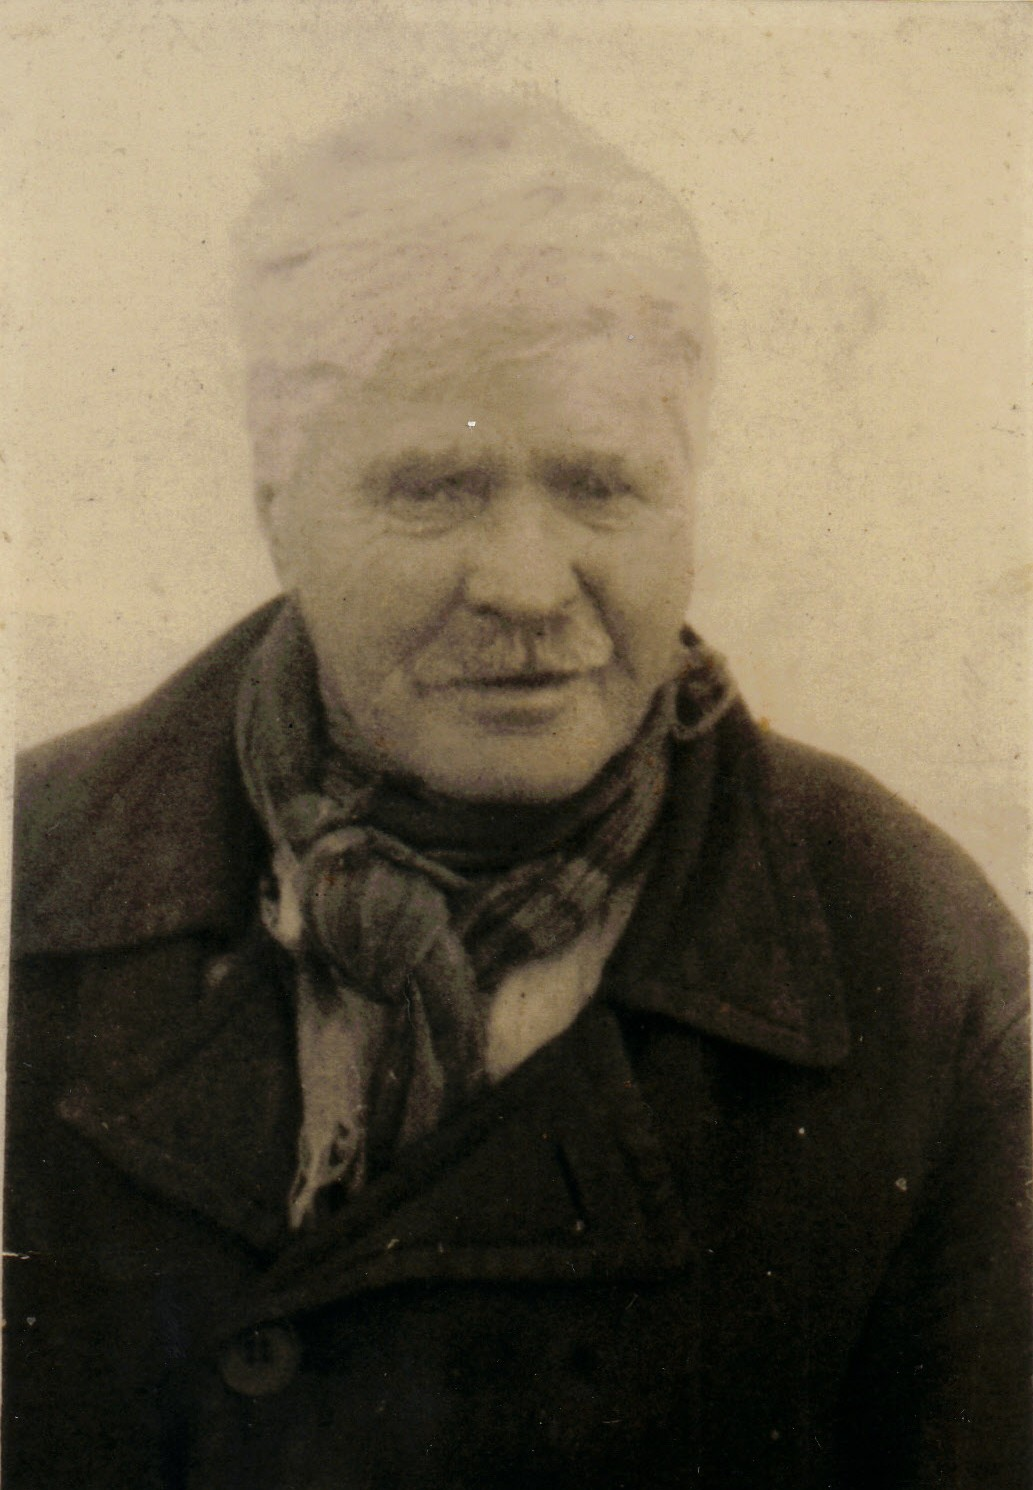
\includegraphics[width=0.4\textwidth]{zdjecia/hilary_lyszczarz.jpg}
\caption{Hilary Łyszczarz}
\label{rys:hilary_lyszczarz}
\end{center}
\end{figure}

A Hilary żył z doskwierającym piętnem ,,bączka'', czyli dziecka z nieprawego łoża aż do 1 czerwca 1945~r. w Mirowie, kiedy to zmarł o godz. 15, w godzinie Miłosierdzia, przeżywszy 66 lat (w akcie zgonu podaje się wiek 62 lat). Była przy jego śmierci ciotka Anielka... Zwykle każdy wiekowy człek dodawał sobie lat, np. Marianna Maciejowa Głąbowa z Hamerlów dodawała dziesięć lat z okładem, skoro w akcie zgonu sporządzonym w 1919 r. podaje się, że miała 94 lata, a urodziła się w 1836 r. Więc sobie  wobec poważnych ludzi dodawała dziesięć lat, a legenda dodała jeszcze dziesięć, skoro Grzesiu Kurek ,,wie'' od swojej matki, że dożyła jej babka stu lat. Dlaczego więc Hilary ujął sobie cztery lata?... Może po to, by zatrzeć ów haniebny rok 1879, gdy jego matka była de iure żoną Macieja (wieść o śmierci męża dotarła do niej dopiero w maju 1882 r.), a wyświetlić prawdopodobieństwo roku 1883, kiedy przyszedł na świat jego młodszy brat Feliks, ale z ojca Smolenia.

,,Żołnierką'' Józefą Łyszczarz (tak nazywano wówczas żony żołnierzy, służących 20 lat w armii carskiej) w 1882 r. zainteresował się bliżej  świeżo upieczony wdowiec po Małgorzacie Kołacz, ale na przeszkodzie stał niewiadomy los jej męża -- Macieja. Więc poprosili pewnie księdza, by u władz rosyjskich dowiedział się o losie Macieja Łyszczarza. Odpowiedź nadeszła 8 maja 1882~r. stwierdzająca zgon Macieja Łyszczarza w ,,Benderskom gospitale'', który nastąpił 30 X 1878~r. W Benderach w Mołdawii, nad Dniestrem Rosjanie mieli twierdzę (ryc.~\ref{rys:akt_zgonu_macieja_lyszczarza}). Od 30 października 1878~r. do 8 V 1882~r. rosyjskie władze nie poczuwały się w obowiązku powiadomić rodzinę o śmierci swego żołnierza. Oto kim dla władz rosyjskich był i jest zwykły żołnierz!


\begin{figure}[!h]
\begin{center}
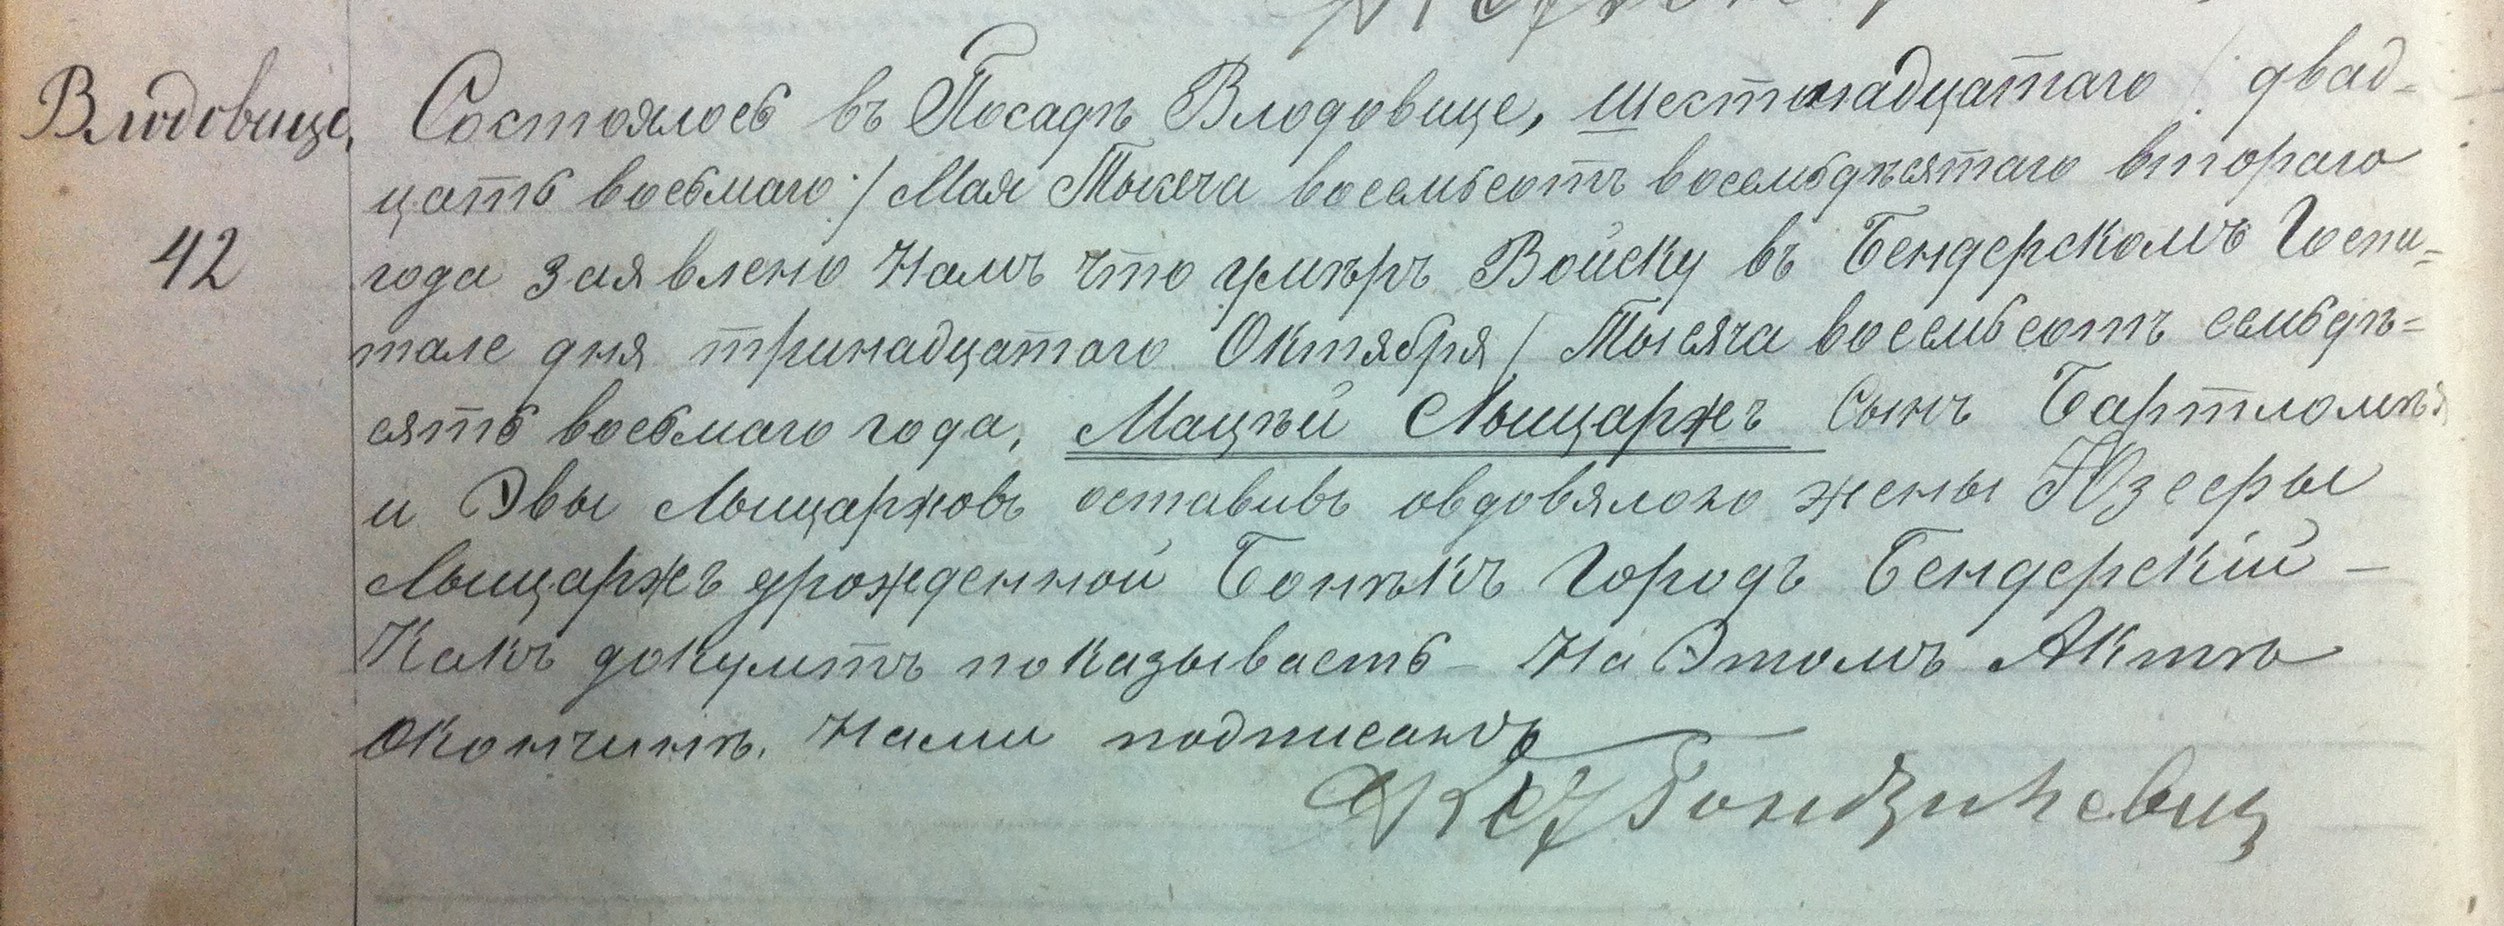
\includegraphics[width=0.8\textwidth]{zdjecia/akt_zgonu_macieja_lyszczarza.jpg}
\caption[Akt zgonu Macieja Łyszczarza]{Akt zgonu Macieja Łyszczarza -- ojca Antoniny Głąb z domu Łyszczarz}
\label{rys:akt_zgonu_macieja_lyszczarza.jpg}
\end{center}
\end{figure}

Pobrali się niemal od razu po otrzymaniu tej wiadomości, która w łagodny sposób rozwiązywała sprawę tolerowania obecności owego ,,bączka'' Hilarego i dawała męską opiekę siedmioletniej wówczas Antosi. Nie była to już jednak opieka miłującego ojca, lecz ojczyma. 29 maja 1882~r. o 4 po południu jej mamusia Józefa (35 lat) z domu Boniek zawarła związek małżeński z Józefem Smoleniem (45 lat) wdowcem, synem Kazimierza i Marianny z domu Czyż (ryc.~\ref{rys:akt_slubu_jozefy_boniek_i_jozefa_smolenia}).

\begin{figure}[!h]
\begin{center}
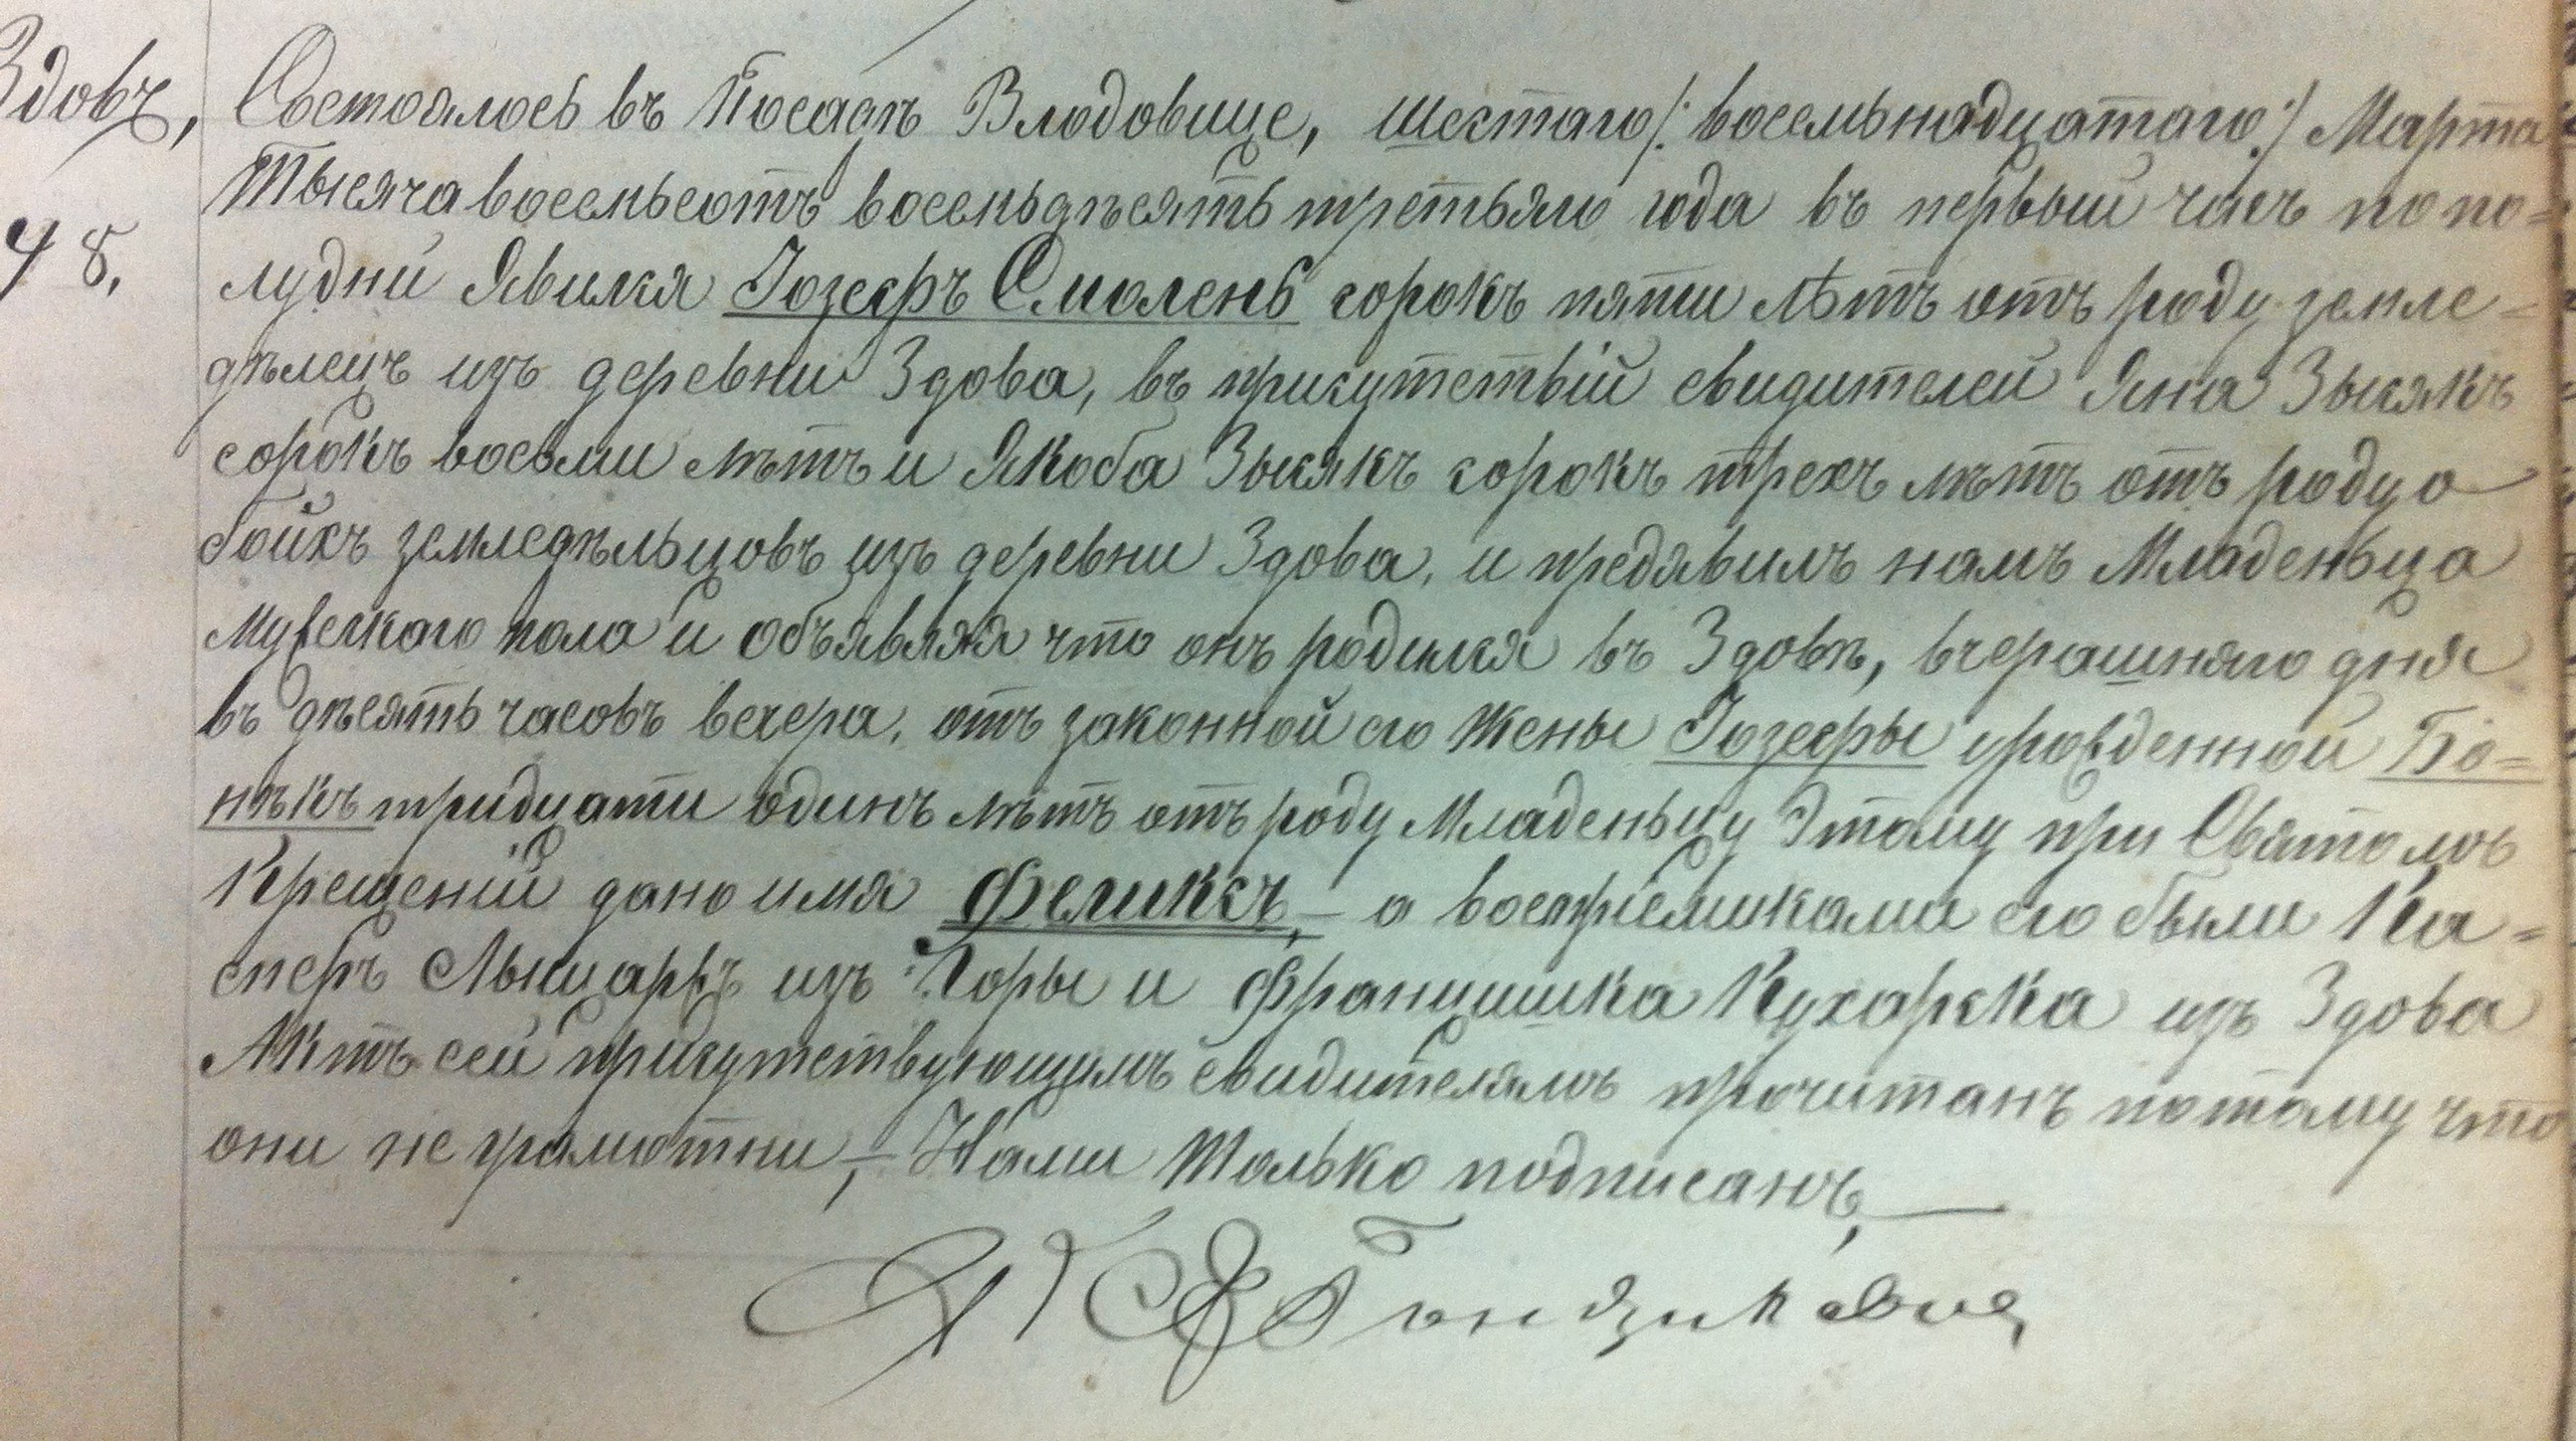
\includegraphics[width=0.8\textwidth]{zdjecia/akt_urodzenia_feliksa_smolenia.jpg}
\caption[Akt urodzenia Feliksa Smolenia]{Akt urodzenia Feliksa Smolenia -- przyrodniego brata Antoniny  Łyszczarz}
\label{rys:akt_urodzenia_feliksa_smolenia}
\end{center}
\end{figure}

\begin{figure}[!h]
\begin{center}
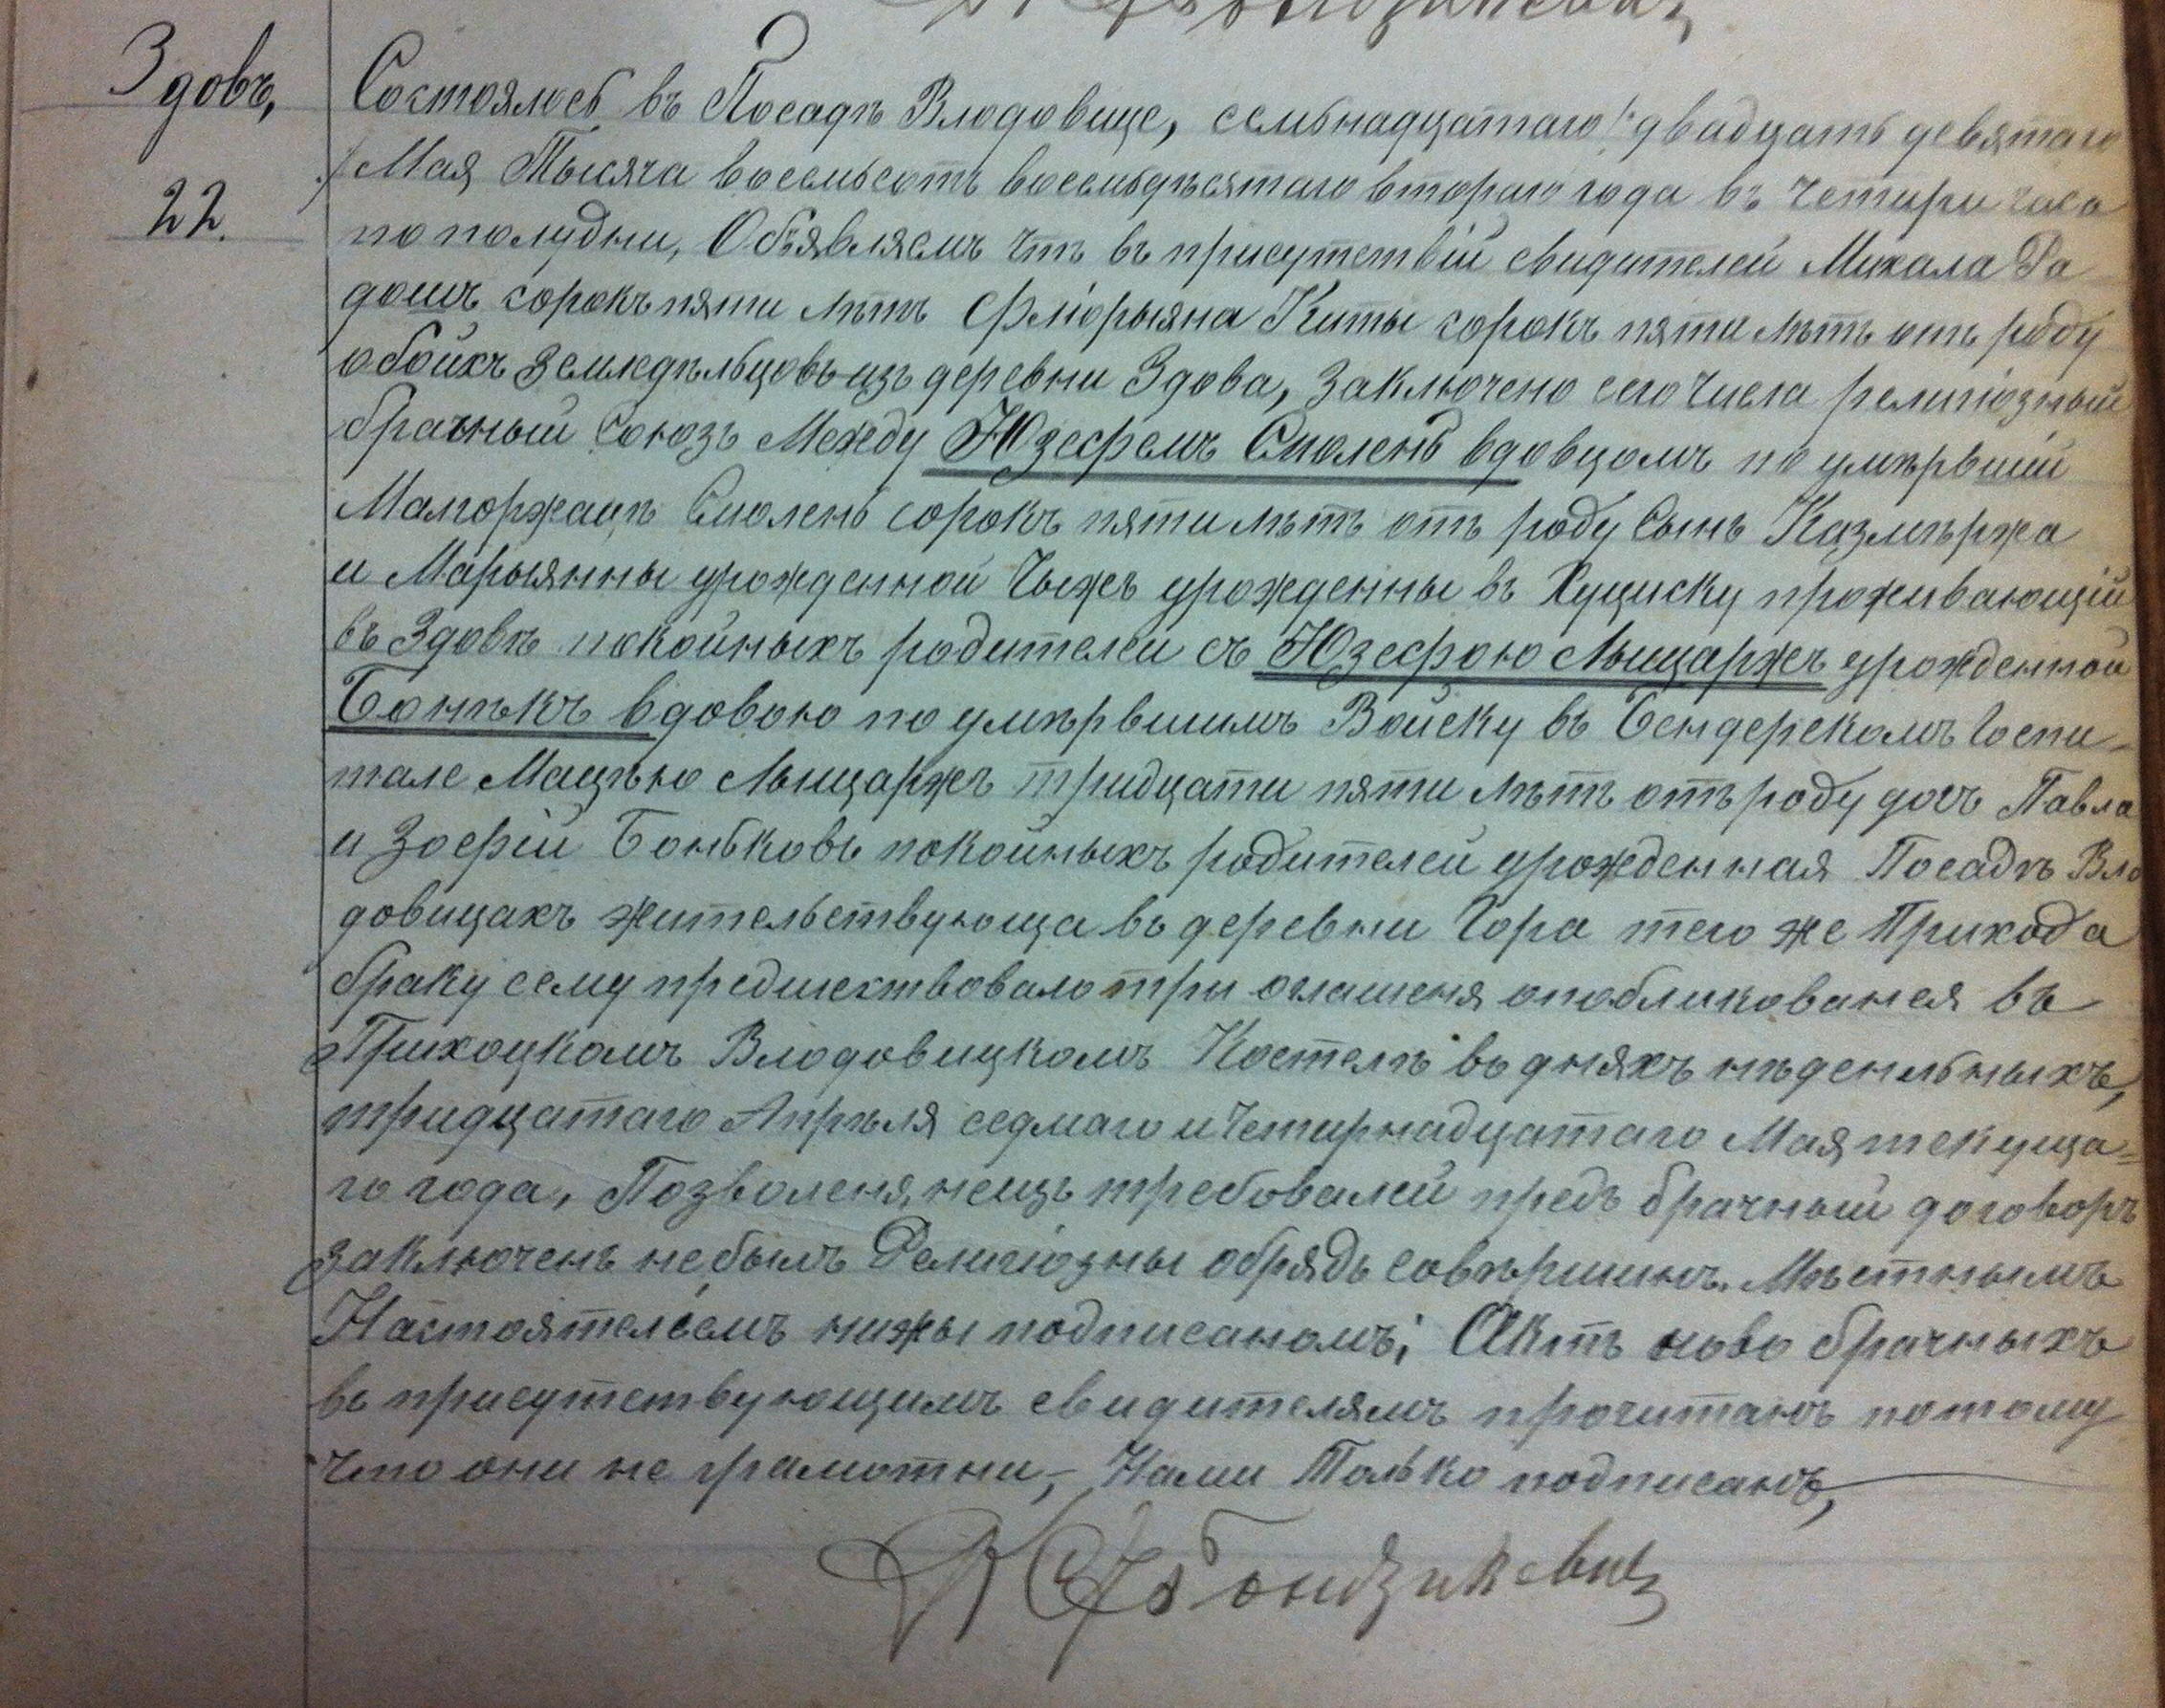
\includegraphics[width=0.8\textwidth]{zdjecia/akt_slubu_jozefy_boniek_i_jozefa_smolenia.jpg}
\caption[Akt ślubu Józefy Boniek z Józefem Smoleniem]{Akt ślubu Józefy Boniek -- matki Antoniny Głąb z domu Łyszczarz, wdowy po Macieju Łyszczarzu z Józefem Smoleniem}
\label{rys:akt_slubu_jozefy_boniek_i_jozefa_smolenia}
\end{center}
\end{figure}

Z tego związku przyszedł na świat 18 marca 1883~r. Feliks Smoleń (ryc.~\ref{rys:akt_urodzenia_feliksa_smolenia}). Jego rodzicami chrzestnymi byli Kasper Łyszczarz z Góry i Franciszka Kucharska ze Zdowa.

Związek Kaspra Łyszczarza z rodziną nieżyjącego już brata Macieja była jak widać żywa, skoro powierzono mu funkcję chrzestnego, na którą się zgodził...

Ów Feliks Smoleń, brat przyrodni (z tej samej matki) naszej Antosi ożenił się 14 lipca 1902~r. jako 19 – letni kawaler z Feliksą Pawulą ze Zdowa, córką nieżyjącego Jakuba i Marianny z Kumorów. Miał z nią dzieci, m.in. syna Feliksa, który mu zmarł w 1918~r.
Wszystko się pięknie zaczęło układać, kiedy śmierć nieubłagana zabrała 16 grudnia 1883~r. Józefę Smoleń -- Łyszczarz z domu Boniek (ryc.~\ref{rys:akt_urodzenia_feliksa_smolenia}). Miała wówczas 36 lat -- córka Pawła Bońka i Zofii z Juszczyków. Zostawiła owdowiałego po raz drugi męża Józefa Smolenia, lecz nade wszystko osierociła troje dzieci z  trzech różnych ojców (a może dwóch, jeśli, kto wie, ojcem Hilarego był Józef Smoleń): Antoninę Łyszczarz z ojca Macieja, Hilarego Łyszczarza – nieznanego ojca oraz Feliksa Smolenia, który został przy ojcu w Zdowie.

\begin{figure}[!h]
\begin{center}
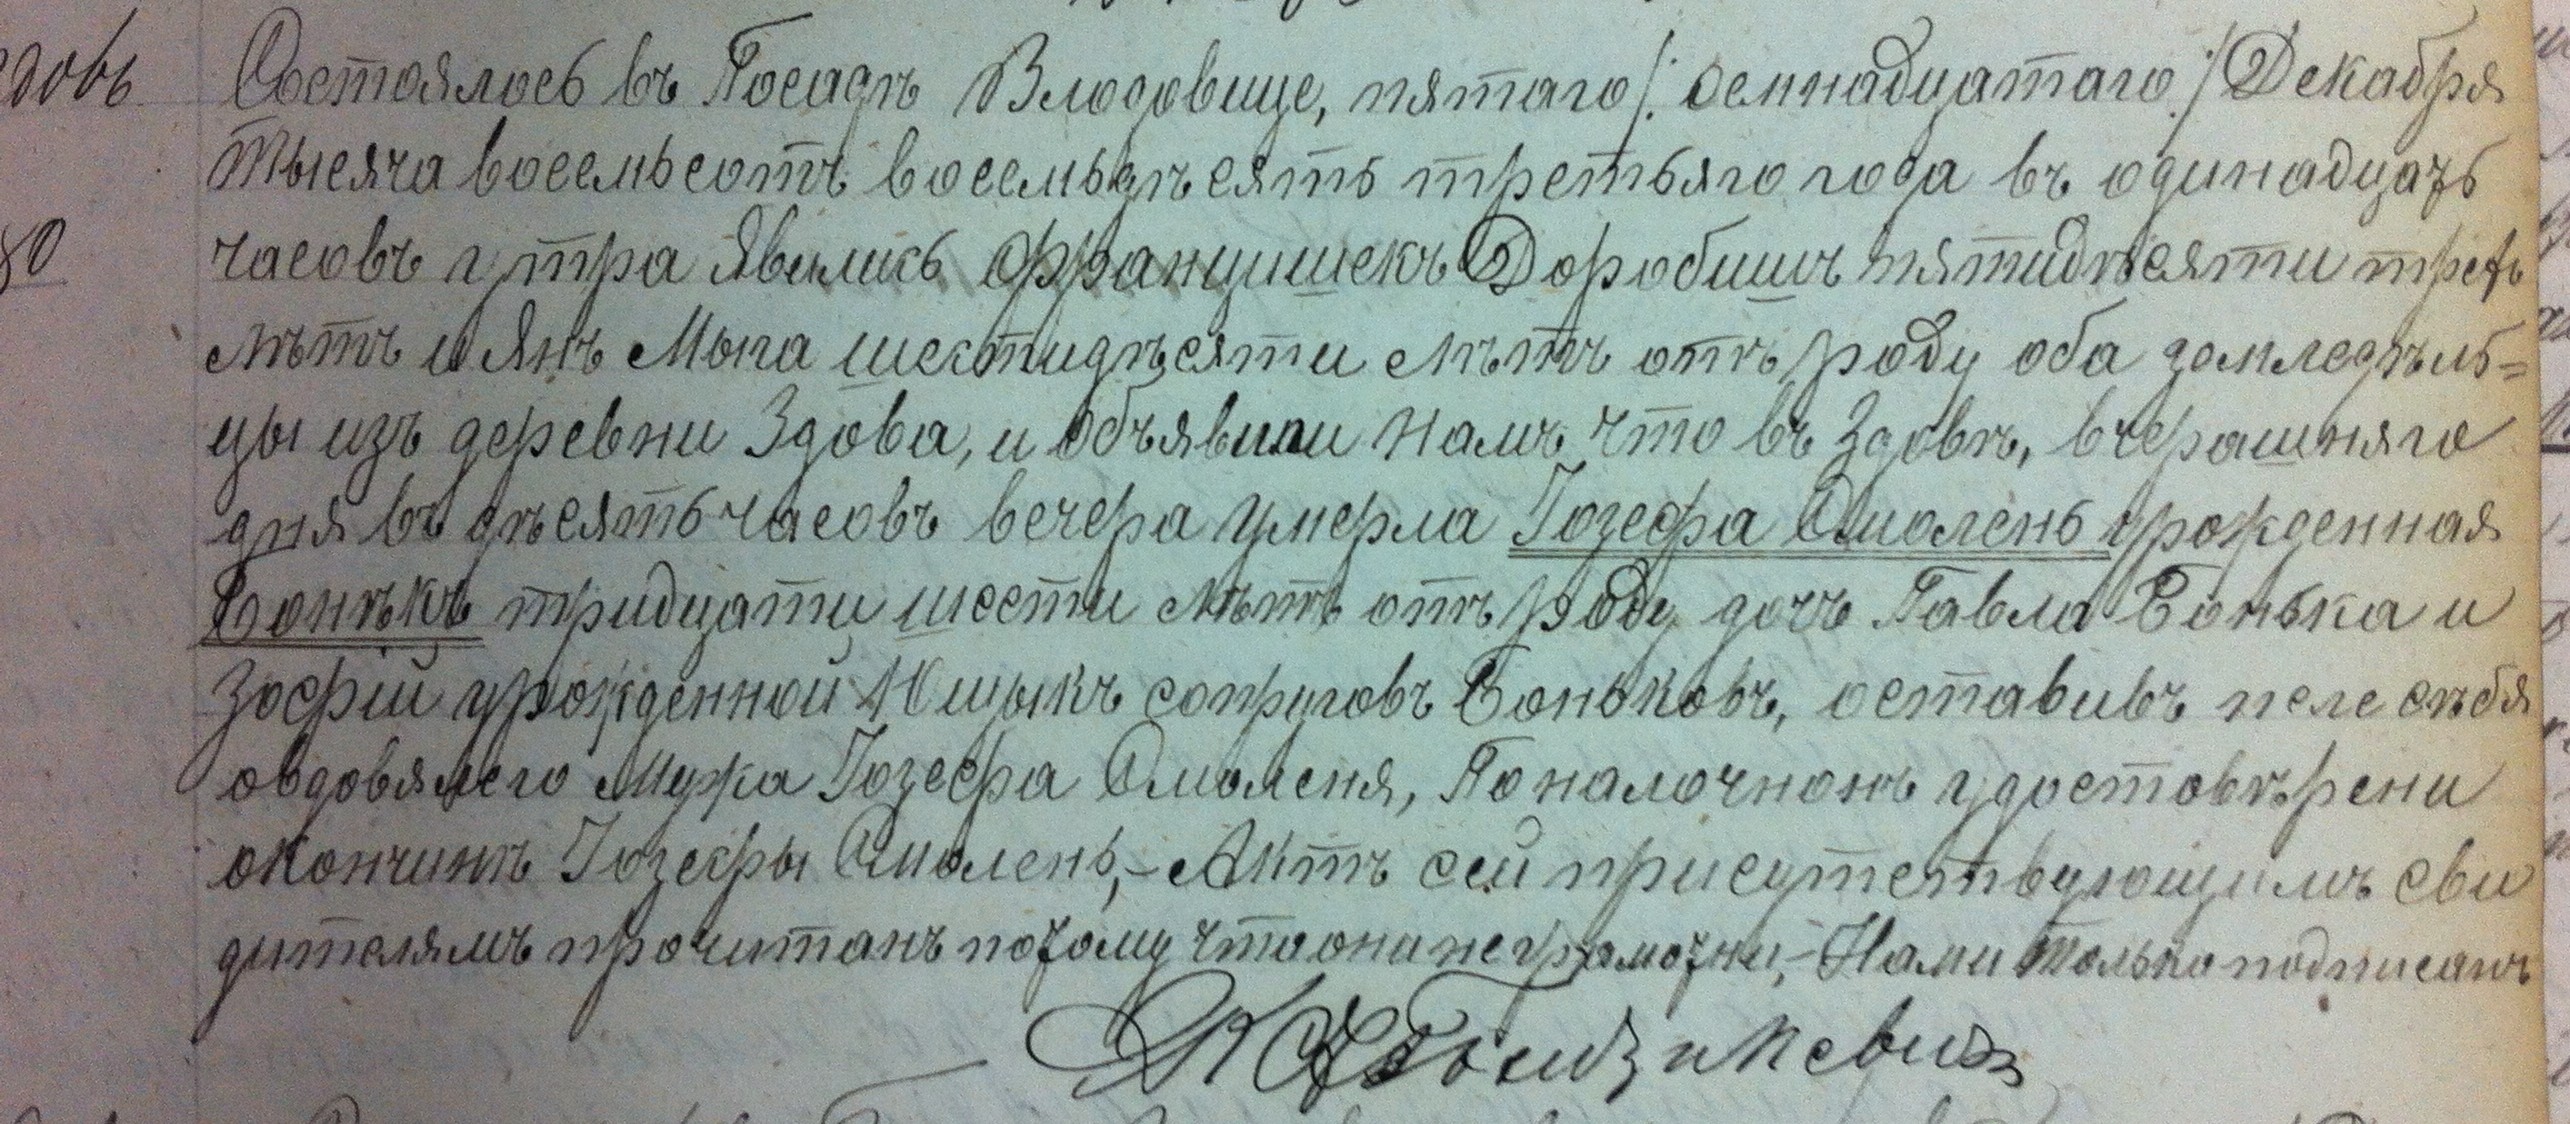
\includegraphics[width=0.8\textwidth]{zdjecia/akt_zgonu_jozefy_boniek.jpg}
\caption{Akt zgonu Józefy Boniek-Łyszczarz-Smoleń -- matki Antoniny Głąb z domu Łyszczarz i Hilarego Łyszczarza oraz Feliksa Smolenia}
\label{rys:akt_zgonu_jozefy_boniek}
\end{center}
\end{figure}

Józef Smoleń najszybciej ze wszystkich otrząsnął się po tej tragedii, bo już 28 stycznia 1884~r. (w półtora miesiąca po śmierci Józefy z Bońków) ożenił się jako 44-letni wdowiec z Barbarą Włoch -- panną lat 19 liczącą, córką Franciszka i Moniki z Zyciaków, urodzoną i mieszkającą przy rodzicach w Zdowie. Tak oto nagle zmieniła się tragicznie sytuacja dziewięcioletniej Antosi i tego pięcioletniego ,,bączka'' Hilarego -- obojga Łyszczarzów, którzy dla Zdowian po śmierci matki -- Józefy Smoleń Łyszczarz Boniek byli obcy. Więc pewnie zabrał ich do siebie Kasper Łyszczarz, który był żonaty i miał już córkę Balbinę, więc przydała się Antosia do opieki nad dwuletnią kuzynką.

\begin{figure}[!h]
\begin{center}
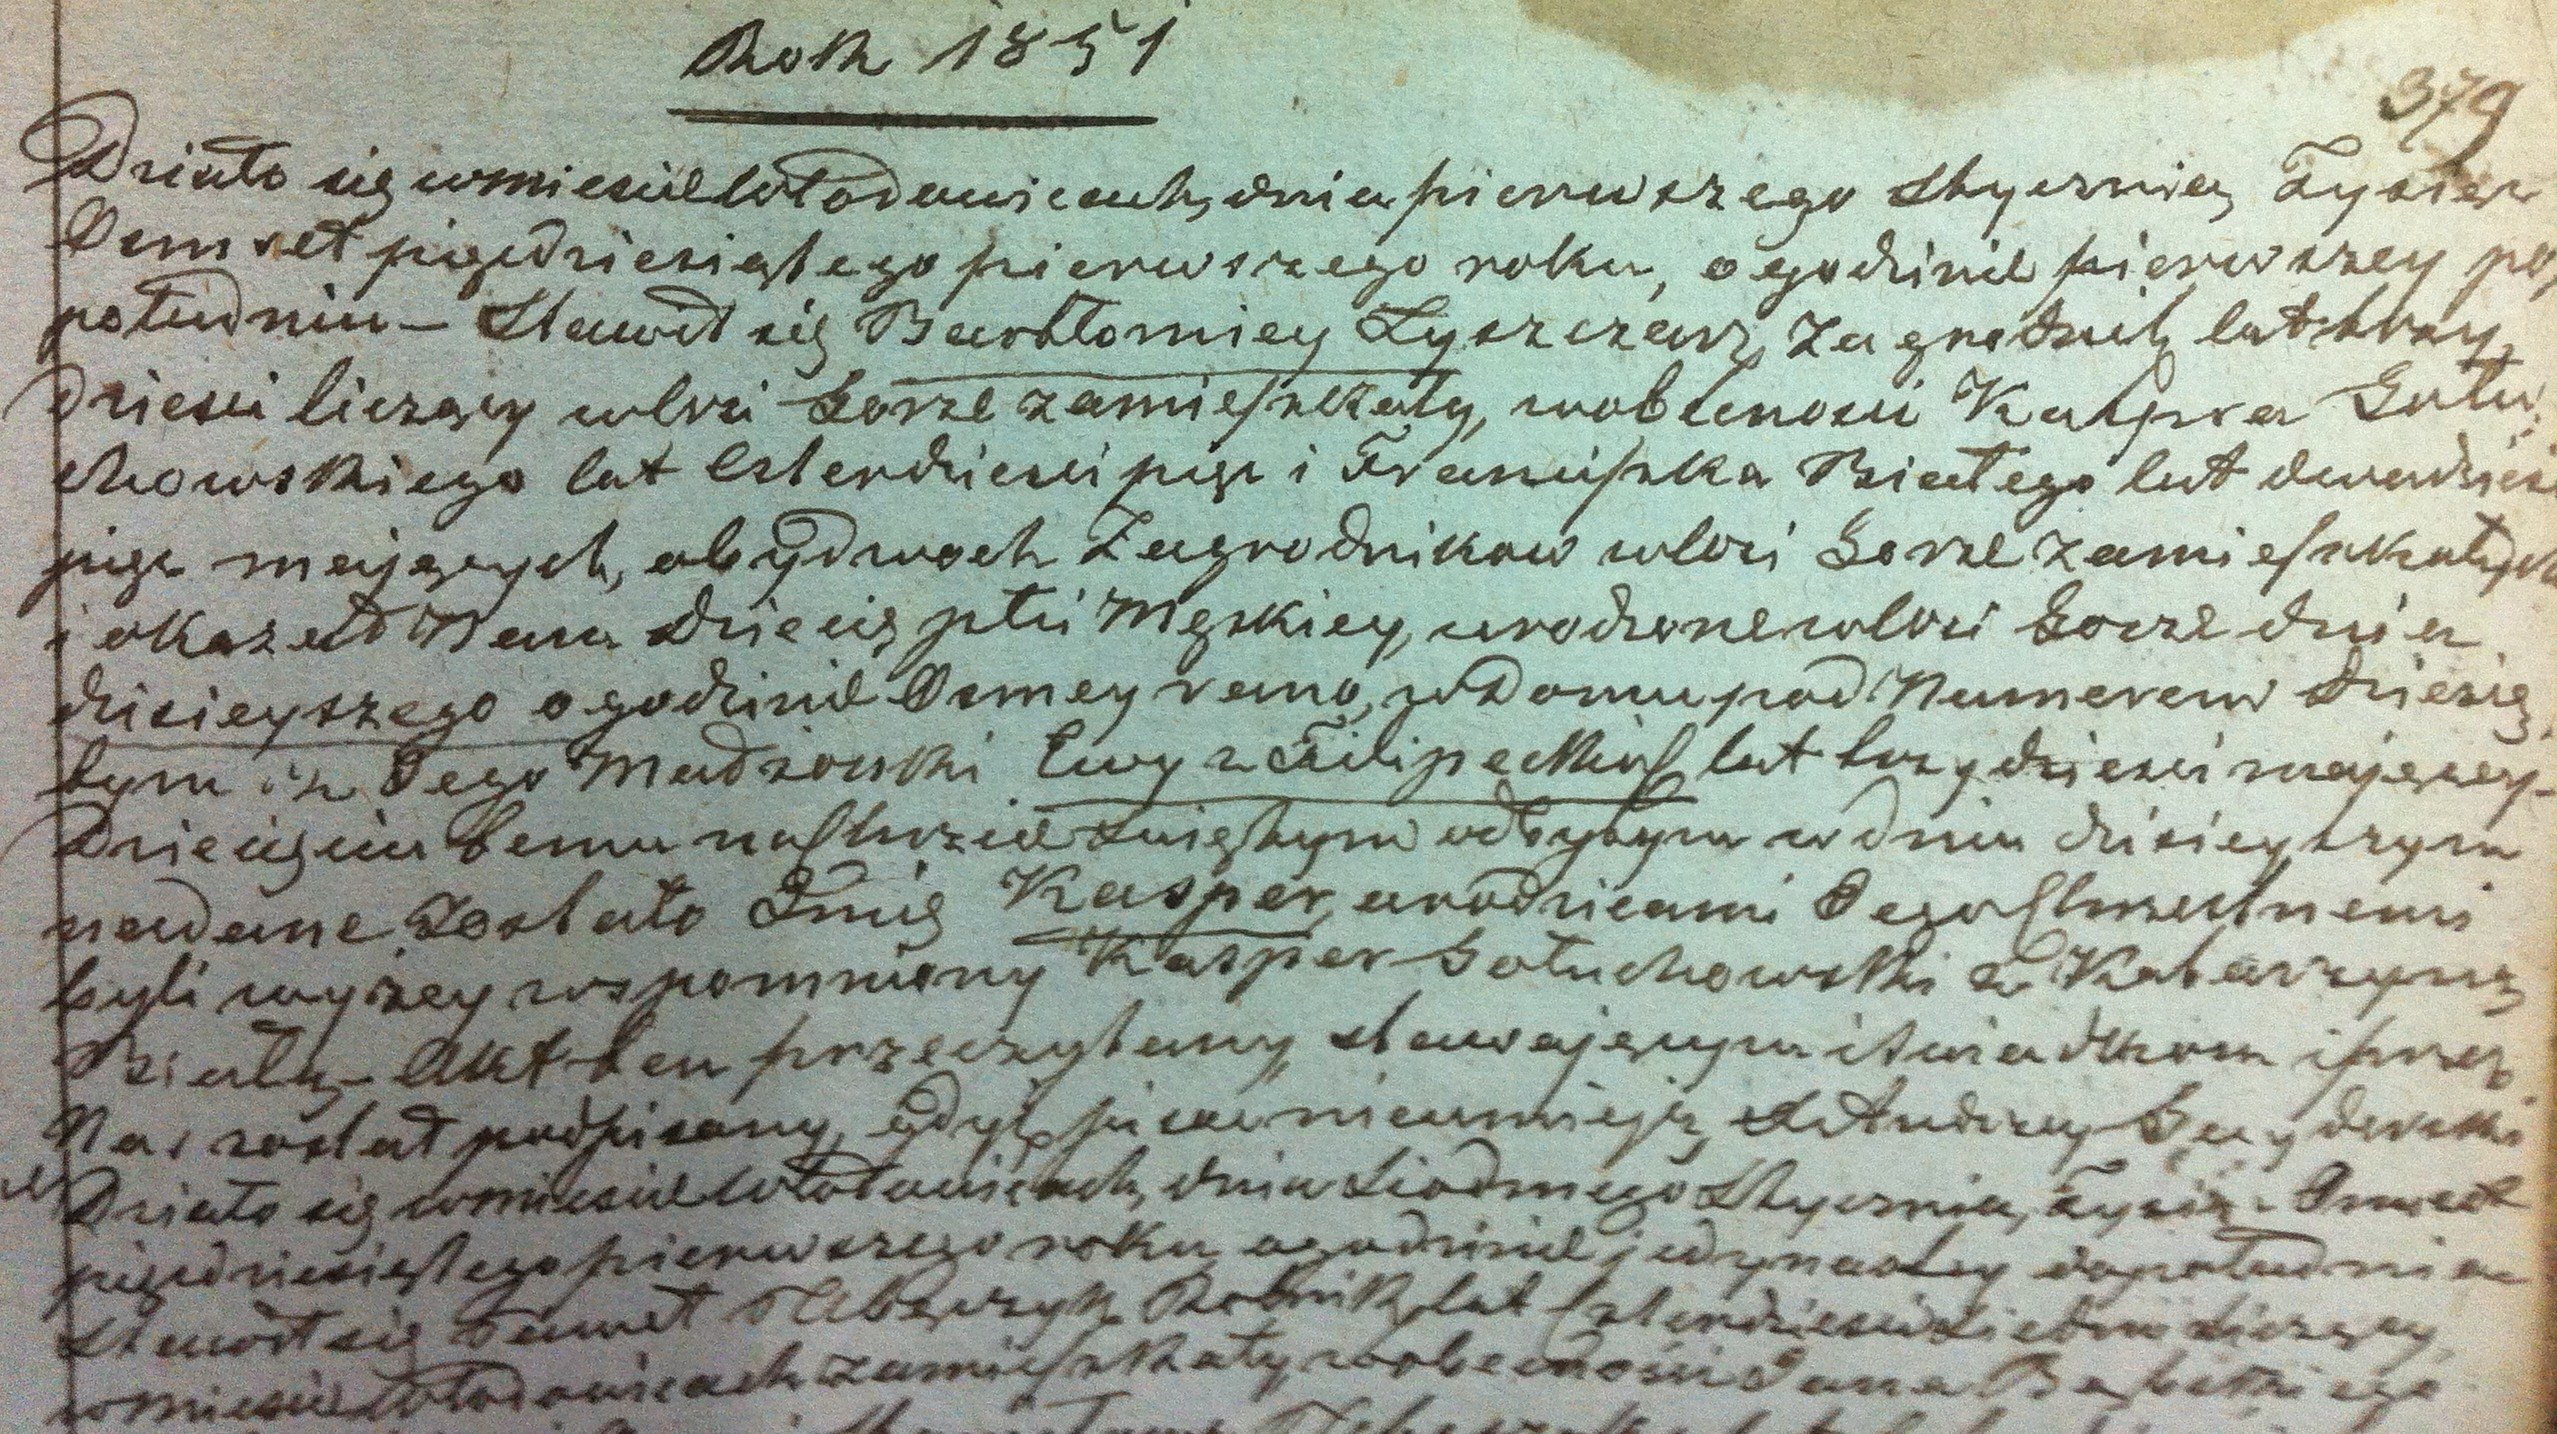
\includegraphics[width=0.8\textwidth]{zdjecia/akt_urodzenia_kaspra_lyszczarza.jpg}
\caption[Akt urodzenia Kaspra Łyszczarza]{Akt urodzenia Kaspra Łyszczarza -- brata ojca Antoniny Głąb z domu Łyszczarz}
\label{rys:akt_urodzenia_kaspra_lyszczarza}
\end{center}
\end{figure}

Musiał ów Józef Smoleń być człowiekiem twardego serca, skoro w półtora miesiąca po śmierci swej kolejnej żony bierze ślub z dziewiętnastoletnią panną ze Zdowa, a zapewne był stroną aktywną w przekazaniu dzieci jego poprzedniej żony bratu jej poprzedniego męża Macieja -- Kasprowi Łyszczarzowi, jeśli wreszcie nie pojawił się na ślubie swej pasierbicy Antoniny we włodowickim kościele, jako że mógł tam być, gdyż ślub ten z Walentym Głąbem odbył się w 1894~r., a Józef Smoleń zmarł 2 stycznia 1896~r. w wieku 60 lat. Był to człek nieciekawej postury skoro dopiero w wieku 33 lat poślubia 42-letnią wdowę -- Małgorzatę Kołaczową z Łyszczarzów, co wydarzyło się 26 VI 1864~r. Zatem urodził się około 1831~r., natomiast w akcie ślubu z Józefą Boniek Łyszczarz zawartym 29 V 1882~r. podaje ów żonkoś, iż ma lat tylko 45, a w istocie pewnie miał lat 51. Gdy zaś bierze 28 I 1884~r. ślub z 19-letnią Barbarą Włoch ma już tylko 44 lata! Trzeba zatem ustalić w życiorysie Józefa Smolenia datę jego urodzenia w Hucisku, bowiem z daty śmierci jego pierwszej żony -- Małgorzaty z Łyszczarzów Kołaczowej, która nastąpiła 7 lutego 1882~r. wynika, że miała wówczas aż 67 lat. Wygląda mi bowiem ów jegomość na taniego oszusta wykorzystującego słabszych dla własnego interesu.

Pora teraz odpowiedzieć na pytanie, kim był dla Antosi ów wyżej wymieniony Kasper Łyszczarz ur. 1 I 1851~r. Był on młodszym bratem jej ojca -- Macieja Łyszczarza (ur. 15 II 1845~r. w Górze), który zmarł w Benderach oraz siostry Franciszki Łyszczarz (ur. 19 II 1843~r.).

W tym czasie Kasper Łyszczarz był już żonaty (od 6 lipca 1880~r.) z panną (wówczas osiemnastoletnią) Antoniną Boniek (jakoś Łyszczarze żon chętnie szukali u Bońków) córką zmarłego Pawła i Marianny z domu Okraska, przy matce mieszkająca we Włodowicach. Owa Antonina Boniek była siostrą przyrodnią Józefy Boniek, lecz z drugiego małżeństwa. Musiał budzić zaufanie u swej bratowej -- Józefy skoro poprosiła go, by był chrzestnym dla jej syna Feliksa.

\begin{figure}[!h]
\begin{center}
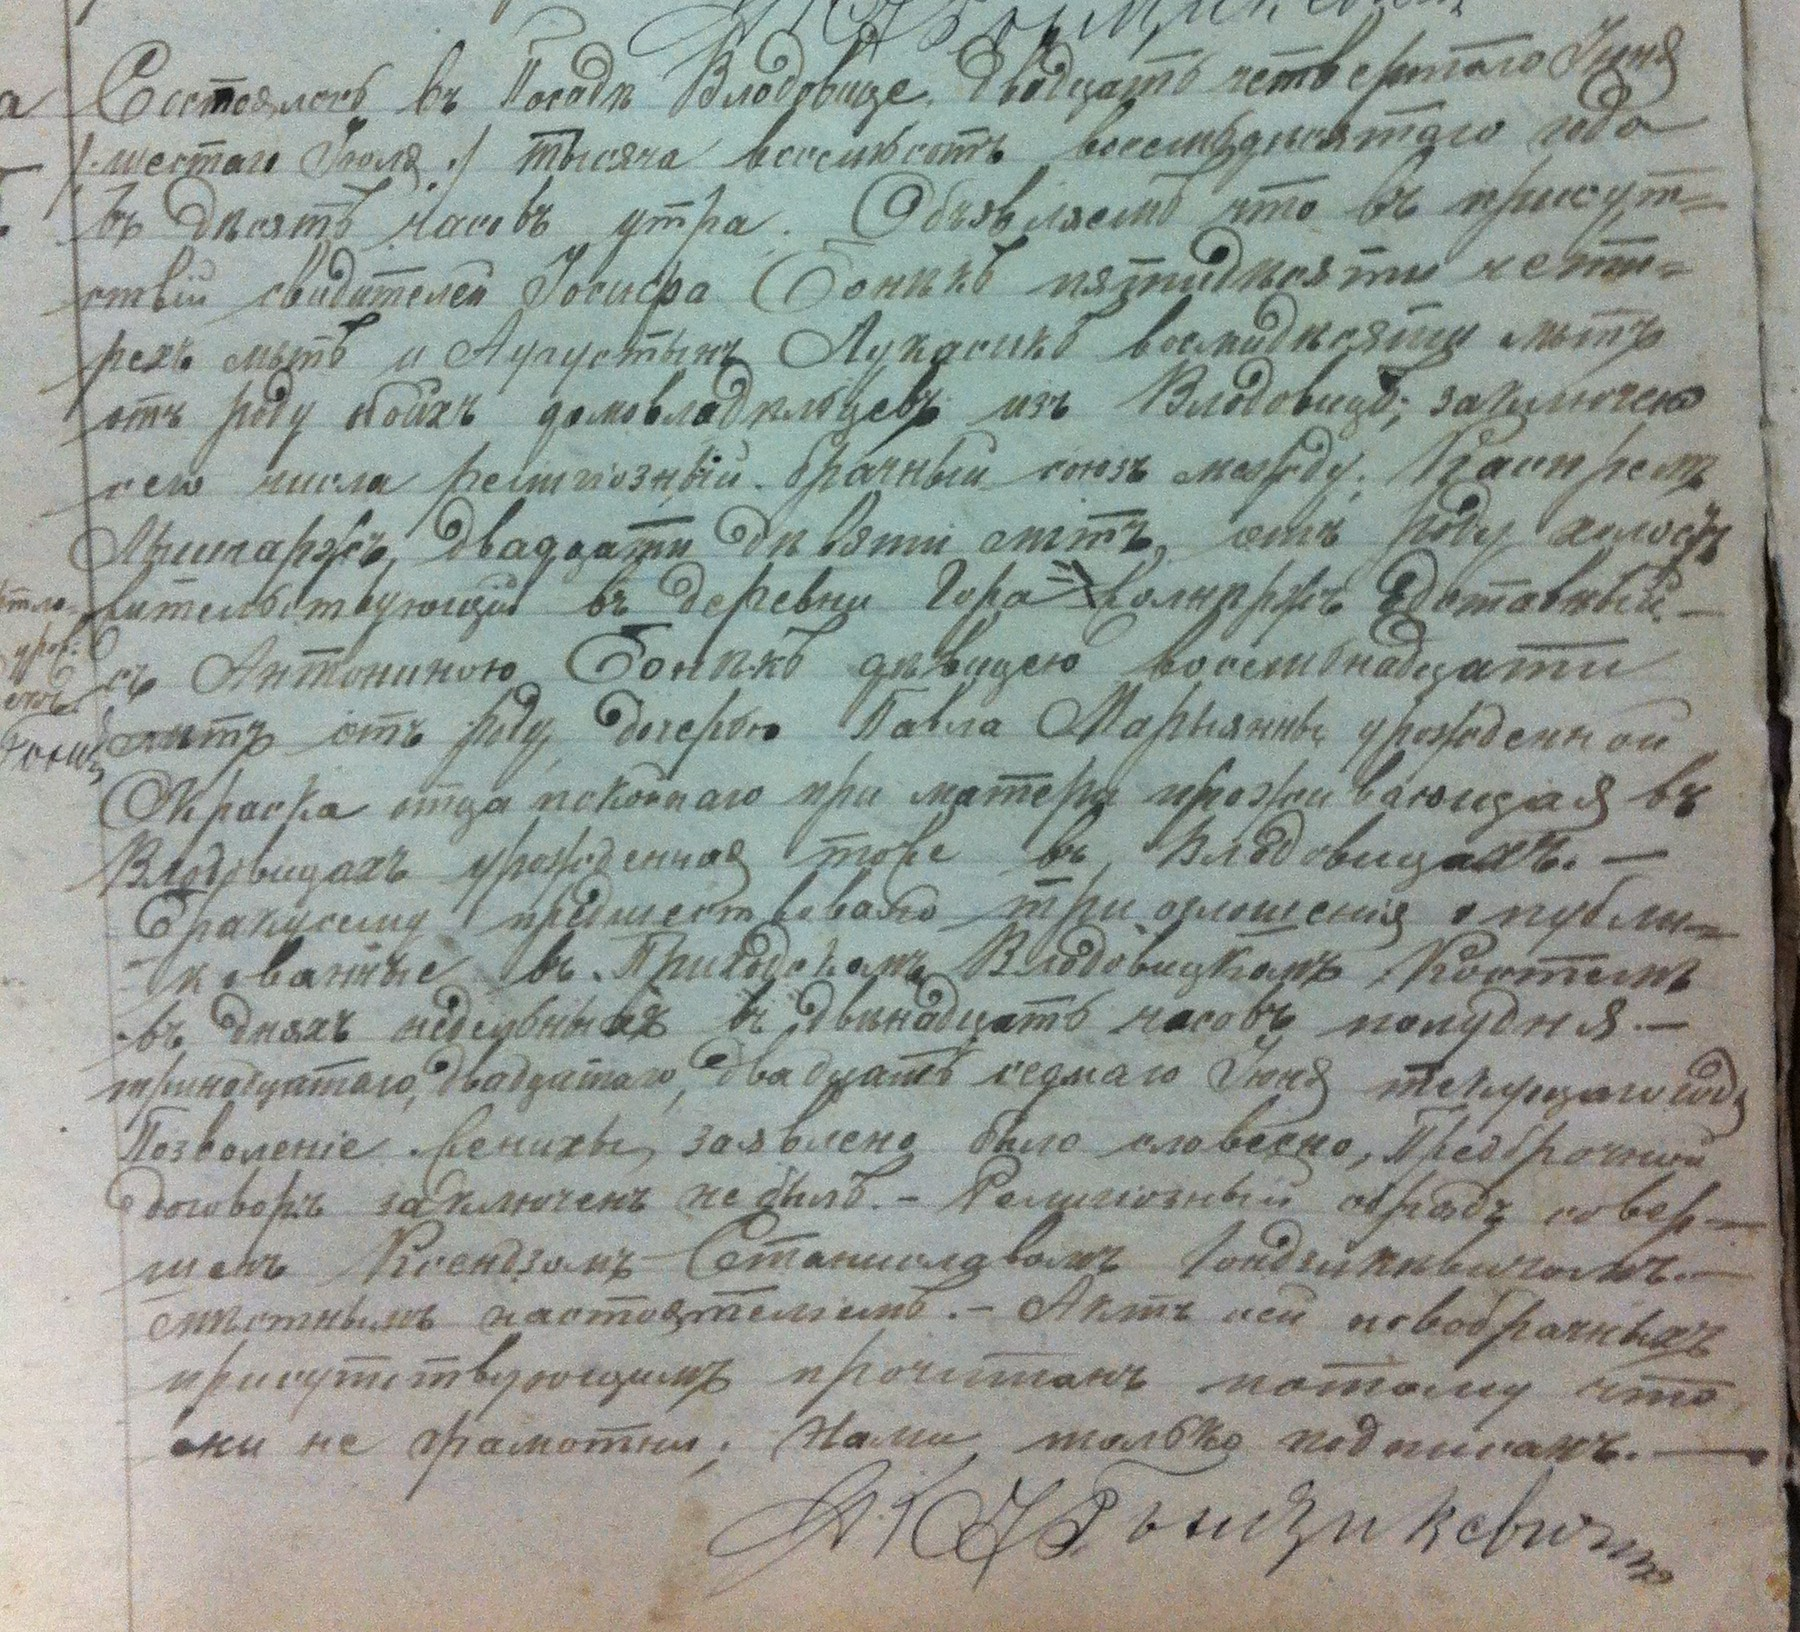
\includegraphics[width=0.7\textwidth]{zdjecia/akt_slubu_kaspra_lyszczarza_i_antoniny_boniek.jpg}
\caption{Akt ślubu Kaspra Łyszczarza (stryja Antoniny Głąb z domu Łyszczarz) z Antoniną Boniek}
\label{rys:akt_slubu_kaspra_lyszczarza_i_antoniny_boniek}
\end{center}
\end{figure}

Podobno nie był on dobry dla swej bratanicy Antoniny, która nie w łóżku, ale na piąstce na przypiecku spała. Jednak gdy przyszło do jej ślubu wyposażył ją na tyle sowicie, że Maciej Głąb zgodził się na ślub swego młodszego syna z zupełną sierotą -- Antoniną Łyszczarz, a ponadto na jej ślubie pełnił funkcję jej prawnego opiekuna. Mało tego, był także ojcem chrzestnym dla Marianny Głąbówny, pierwszej córki swej bratanicy!

Maciej i Kasper Łyszczarzowie byli, jako się rzekło, braćmi z ojca Bartłomieja Łyszczarza ur. 10 sierpnia 1821~r. w Górze Włodowskiej.


\begin{figure}[!h]
\begin{center}
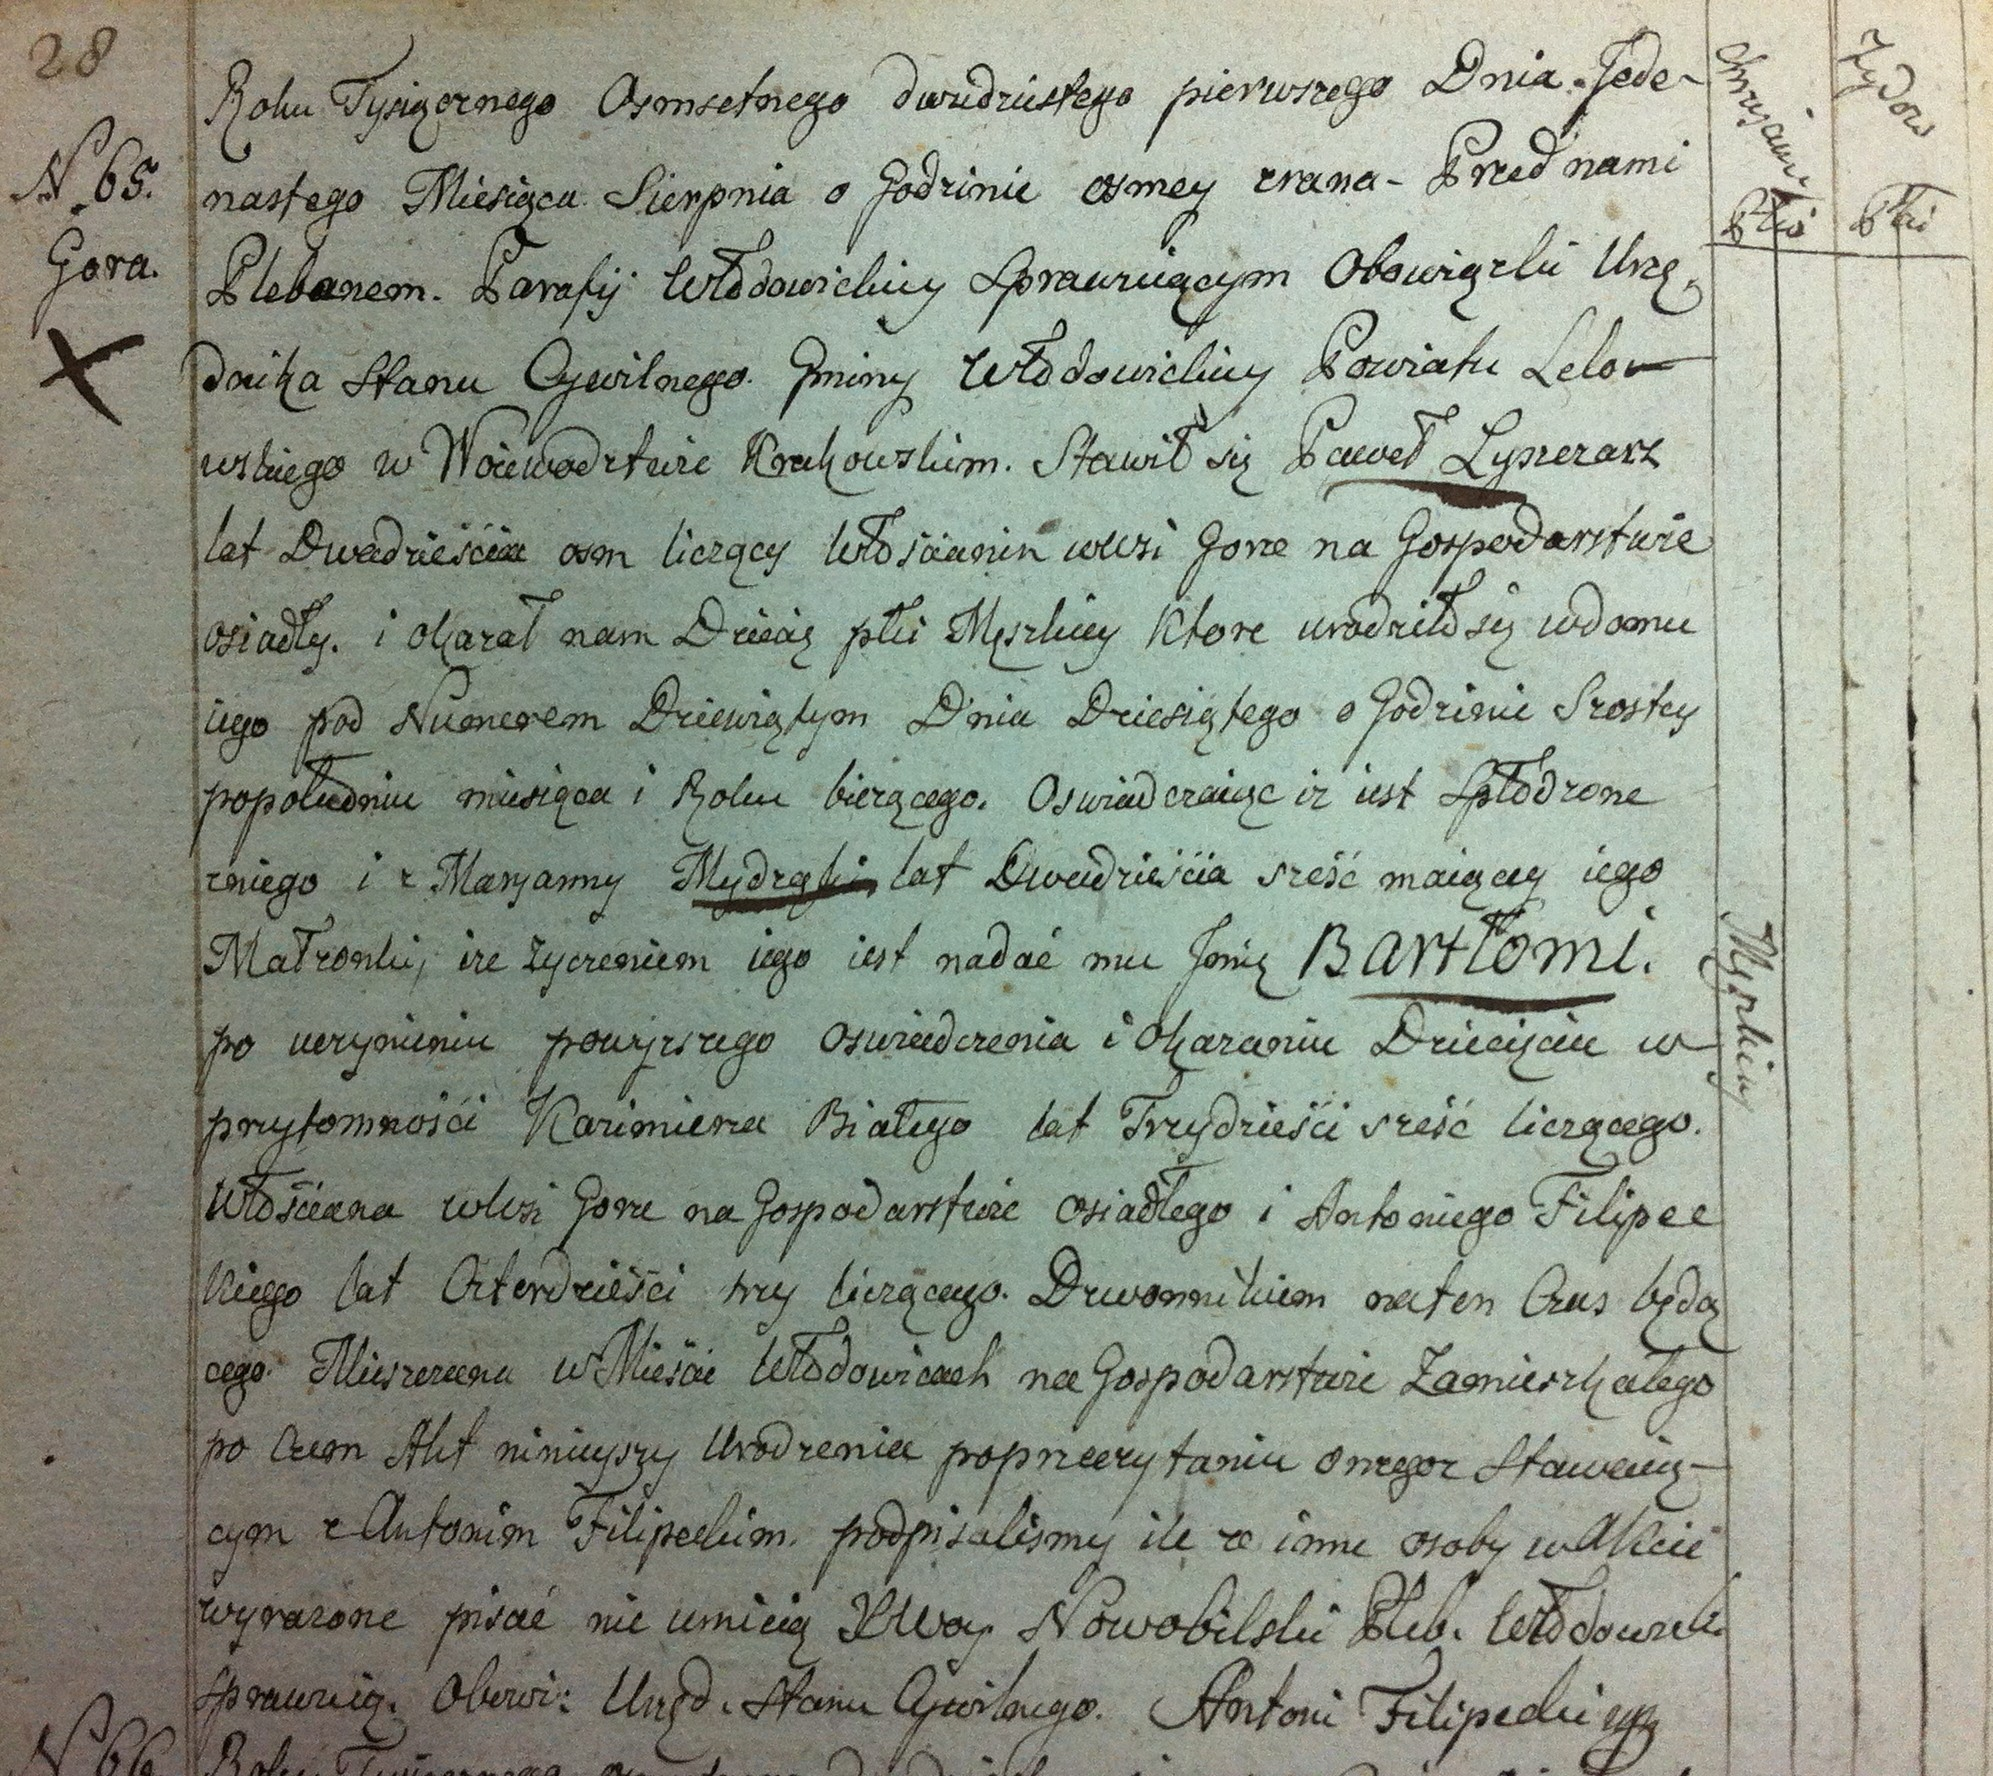
\includegraphics[width=0.7\textwidth]{zdjecia/akt_urodzenia_bartlomieja_lyszczarza.jpg}
\caption[Akt urodzenia Bartłomieja Łyszczarza]{Akt urodzenia Bartłomieja Łyszczarza -- dziadka Antoniny Głąb z domu Łyszczarz}
\label{rys:akt_urodzenia_bartlomieja_lyszczarza}
\end{center}
\end{figure}

Zmarł on już 8 IV 1860~r. w Górze Włodowskiej, miał więc w chwili śmierci 39 lat, a jego syn Maciej lat 15, młodszy Kasper ur. 1 I 1851~r. miał lat dziewięć, a jeszcze młodszy Andrzej ur. 12 XI 1853~r. miał lat siedem.

%TODO *** Tu zdj. aktu zgonu Bartłomieja Łyszczarza; zdj. nr 292 w pliku Archiwum diecezj.}

Rodzice Macieja i Kaspra pobrali się 8 II 1841~r. we Włodowicach. Ich matka Ewa z Filipeckich zmarła 24 XI 1872~r. w wieku 52 lat, gdy synowie byli już pełnoletni, lecz gdy się żenili byli zupełnymi sierotami.

\begin{figure}[!h]
\begin{center}
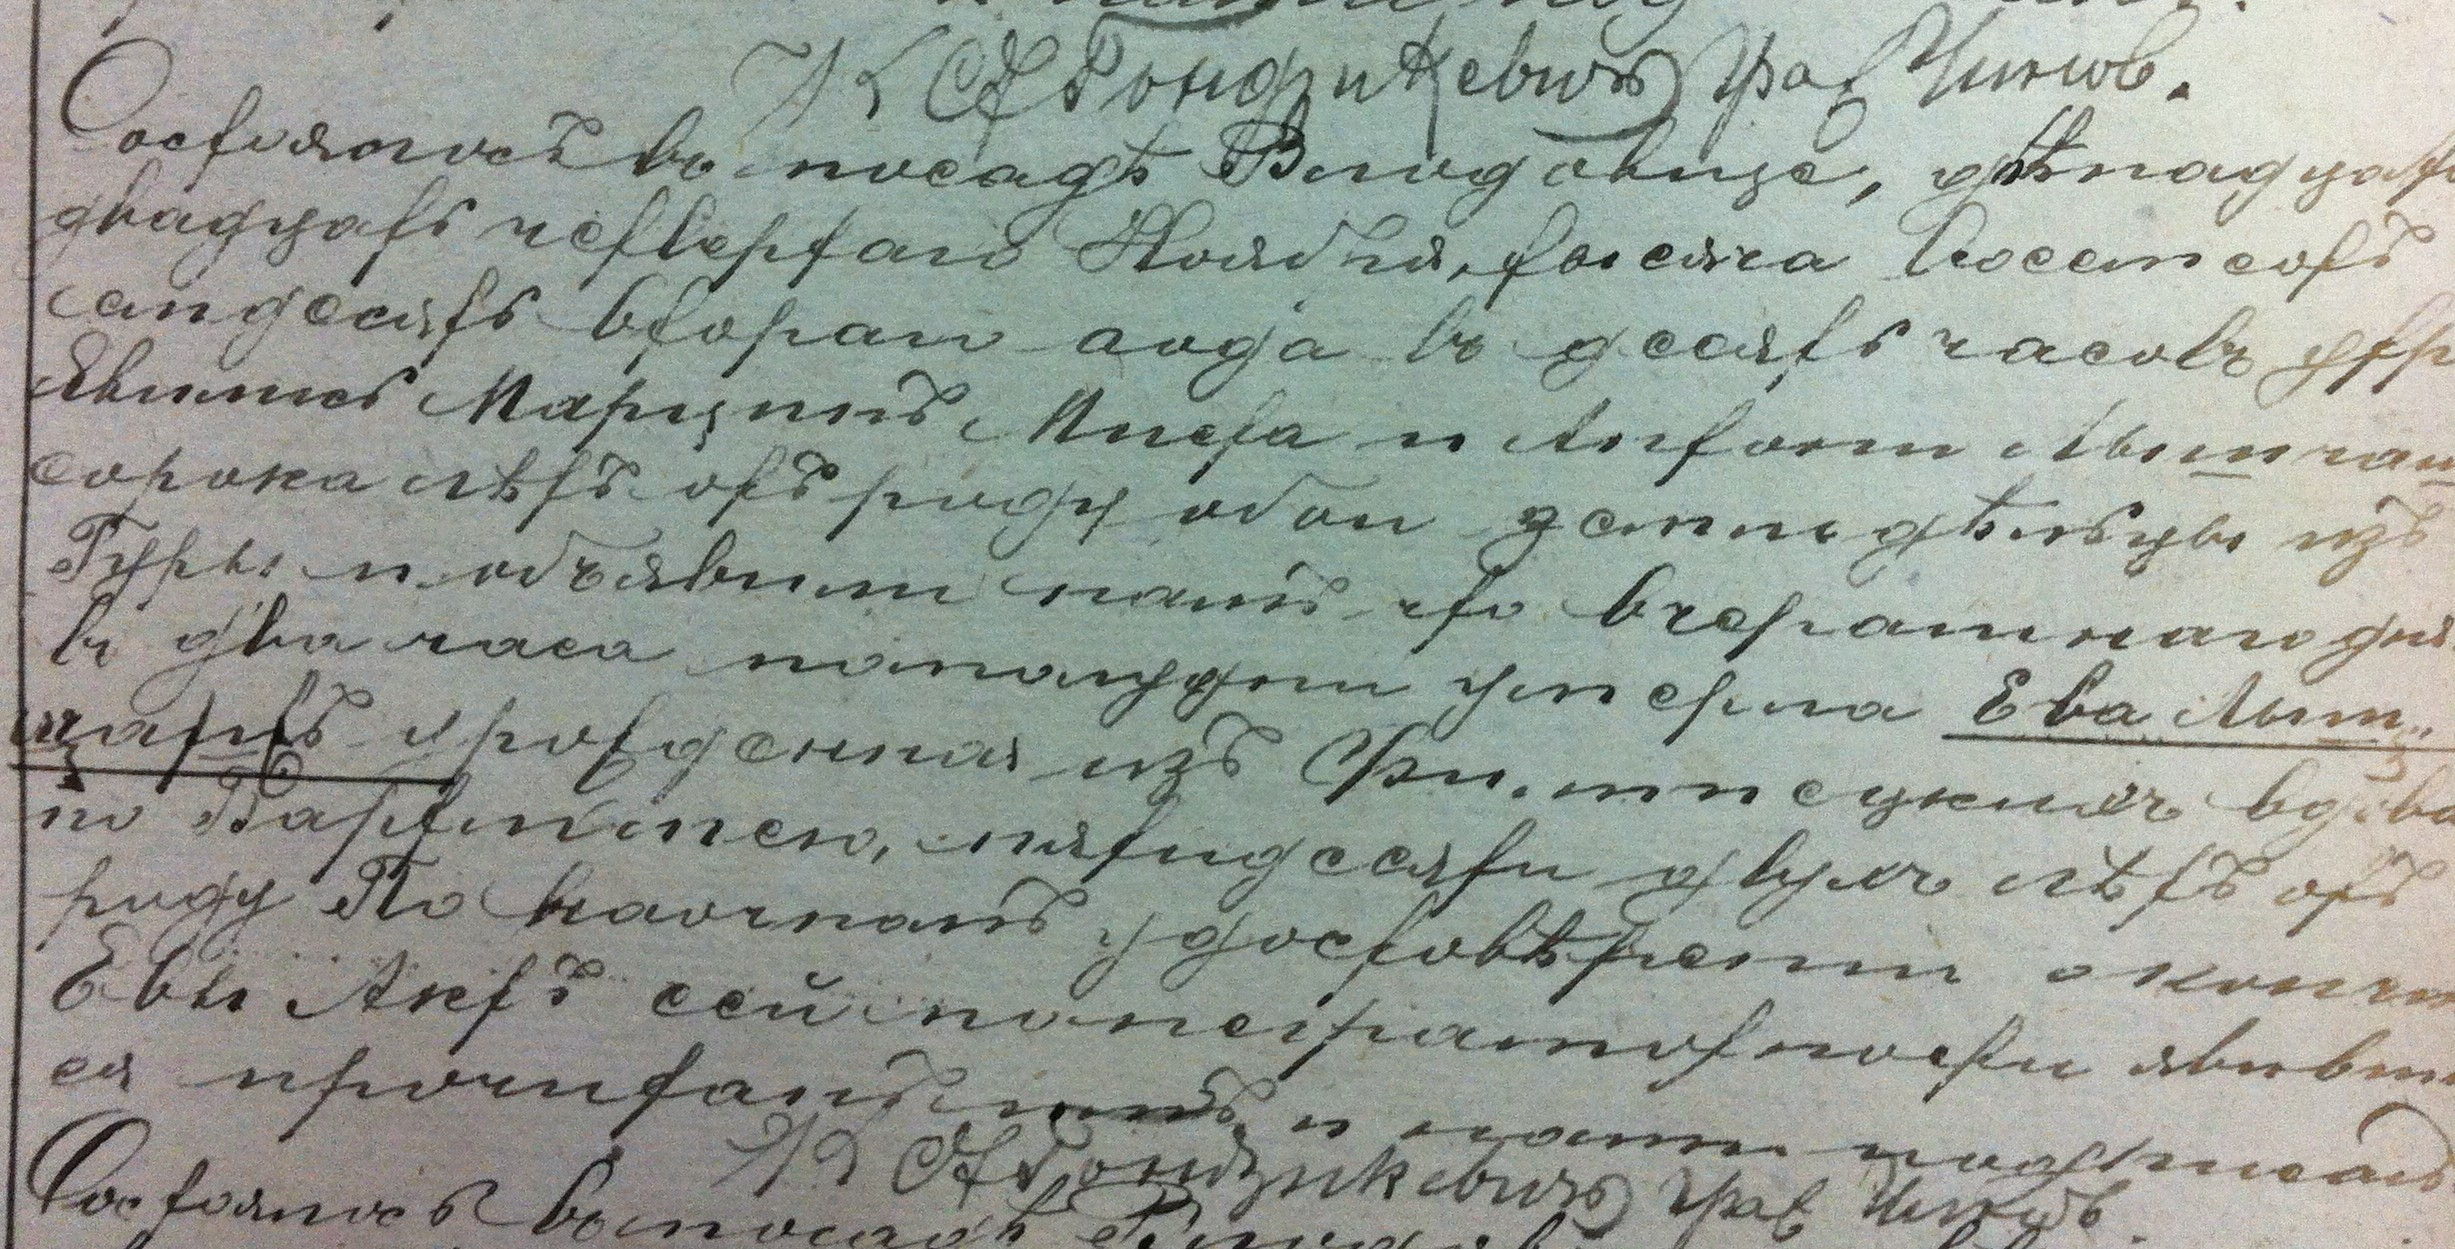
\includegraphics[width=0.8\textwidth]{zdjecia/akt_zgonu_ewy_lyszczarz.jpg}
\caption[Akt zgonu Ewy Łyszczarz z domu Filipeckiej]{Akt zgonu Ewy Łyszczarz z domu Filipeckiej -- babki Antoniny Głąb z domu Łyszczarz}
\label{rys:akt_zgonu_ewy_lyszczarz}
\end{center}
\end{figure}

Również Józefa Boniek -- matka Antoniny Łyszczarz, ur. 18 III 1851~r. we Włodowicach z ojca Pawła Bońka (ur. 7 I 1820~r. we Włodowicach z ojca Kazimierza i matki Agnieszki z Piaseckich) i matki Zofii Juszczyk (ur. 22 IV 1821~r. we Włodowicach z ojca Idziego Juszczykowskiego i matki Elżbiety Wcisło) bardzo wcześnie utraciła matkę.

\begin{figure}[!h]
\begin{center}
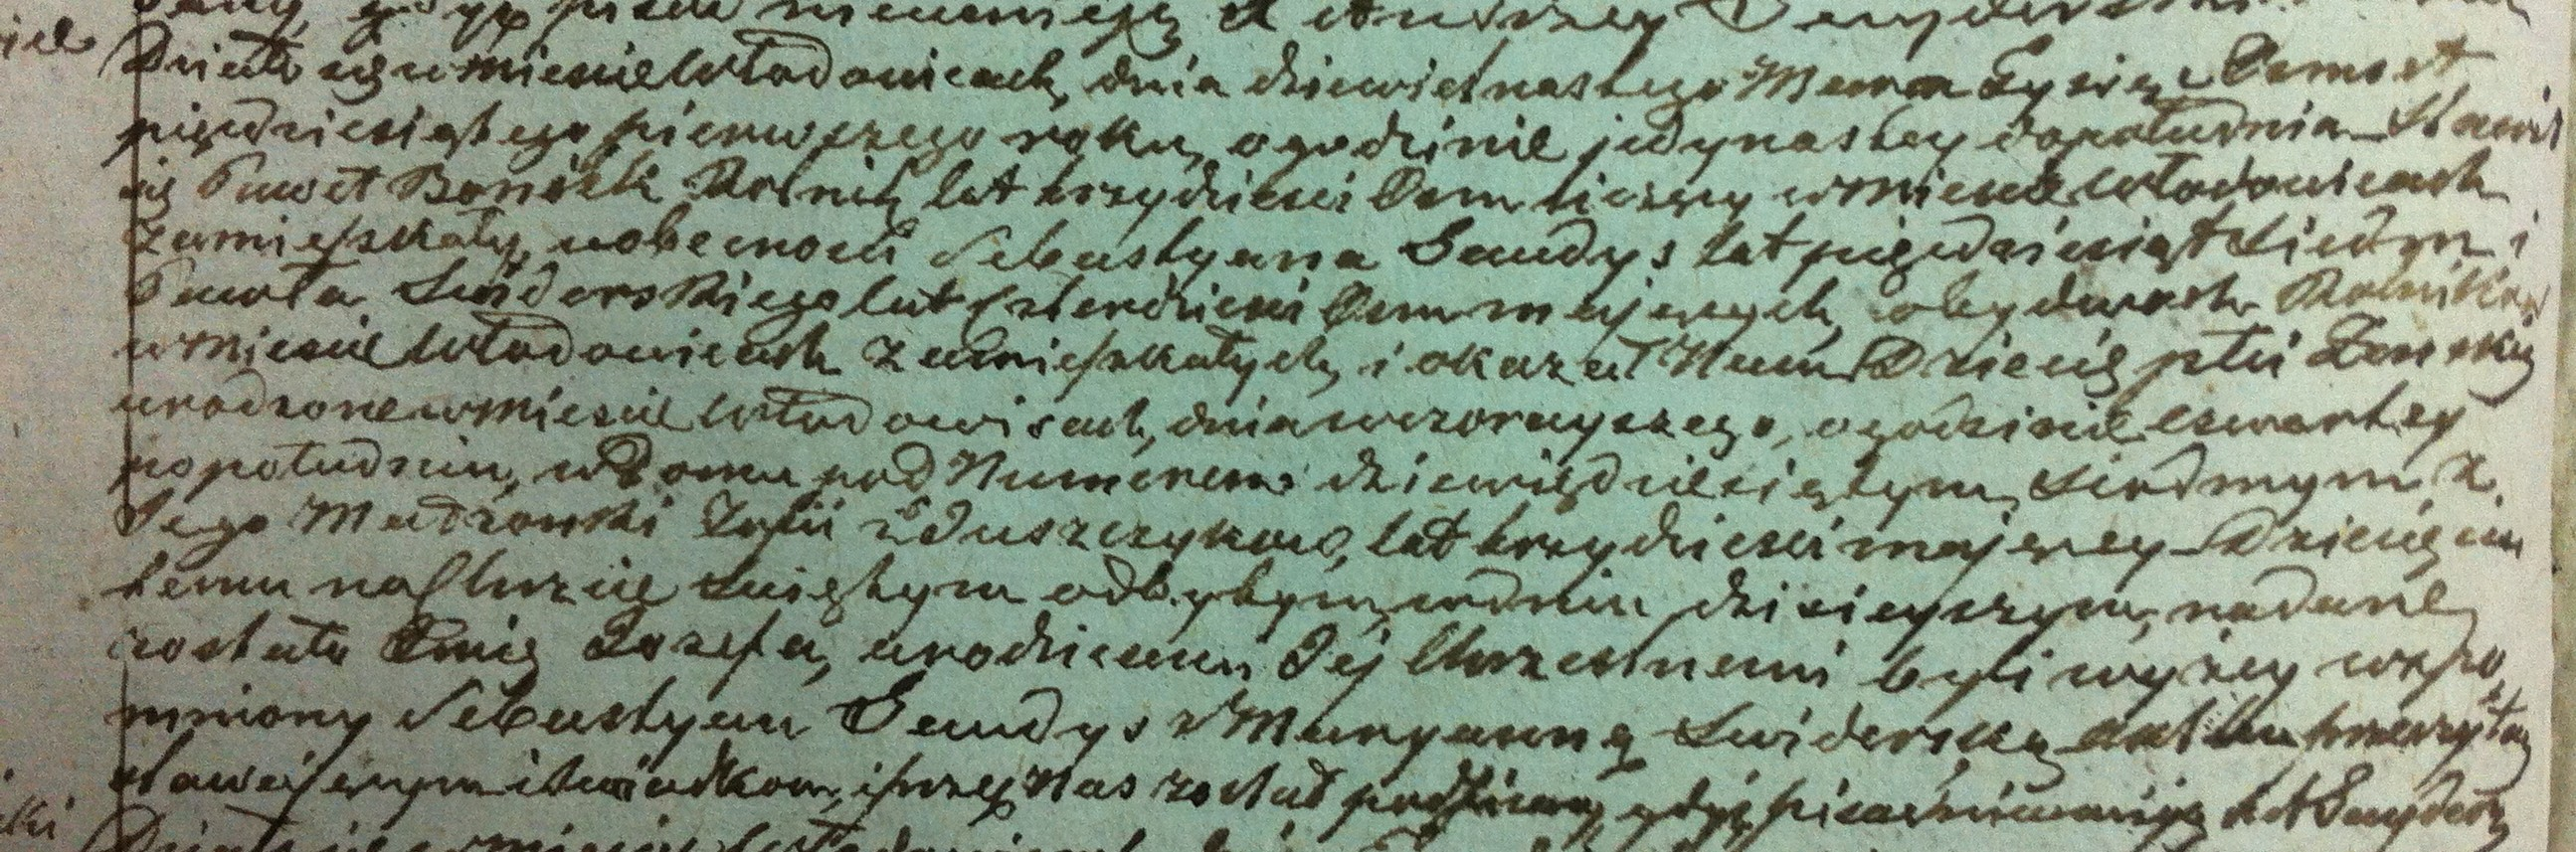
\includegraphics[width=0.8\textwidth]{zdjecia/akt_urodzenia_jozefy_boniek.jpg}
\caption[Akt urodzenia Józefy Boniek]{Akt urodzenia Józefy Boniek -- matki Antoniny Głąb z domu Łyszczarz}
\label{rys:akt_urodzenia_jozefy_boniek}
\end{center}
\end{figure}

Zofia Boniek z Juszczyków zmarła bowiem już 10 listopada 1857~r., gdy Józefa miała zaledwie 6 lat!

\begin{figure}[!h]
\begin{center}
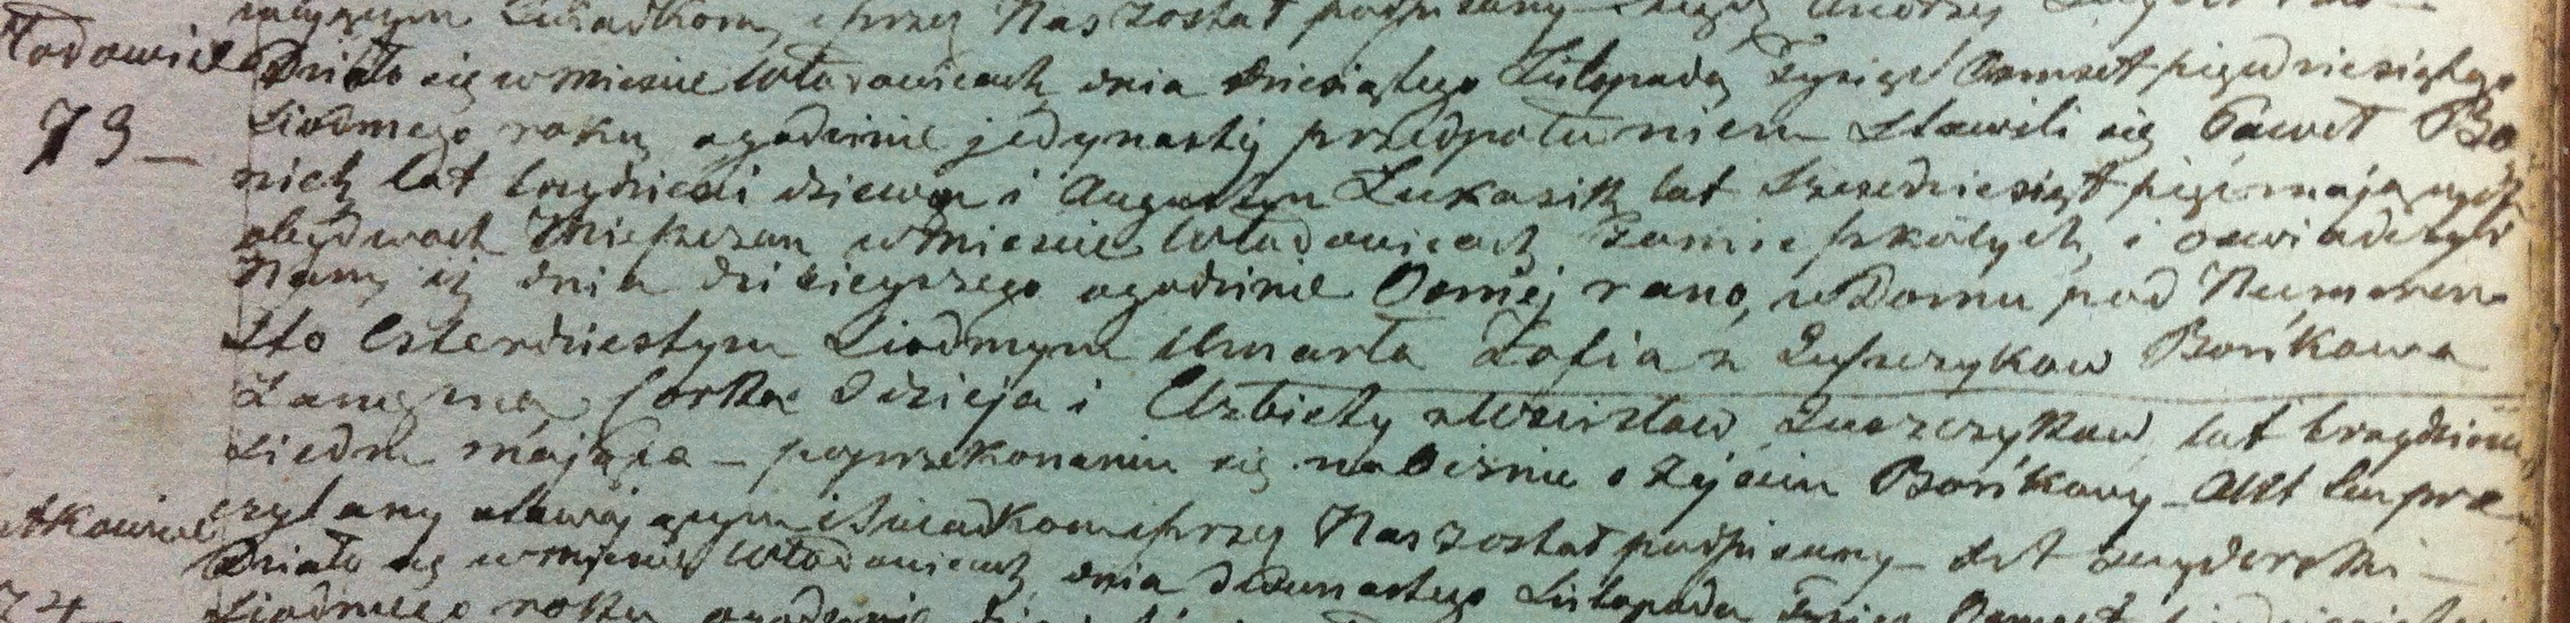
\includegraphics[width=0.8\textwidth]{zdjecia/akt_zgonu_zofii_boniek.jpg}
\caption[Akt zgonu Zofii Boniek]{Akt zgonu Zofii Boniek z domu Juszczyk -- babki Antoniny Głąb z domu Łyszczarz}
\label{rys:akt_zgonu_zofii_boniek.jpg}
\end{center}
\end{figure}

Jej tatuś ożenił się powtórnie już w trzy miesiące później, tj. 7 lutego 1858~r. we Włodowicach z Marianną Okraską. 


\begin{figure}[!h]
\begin{center}
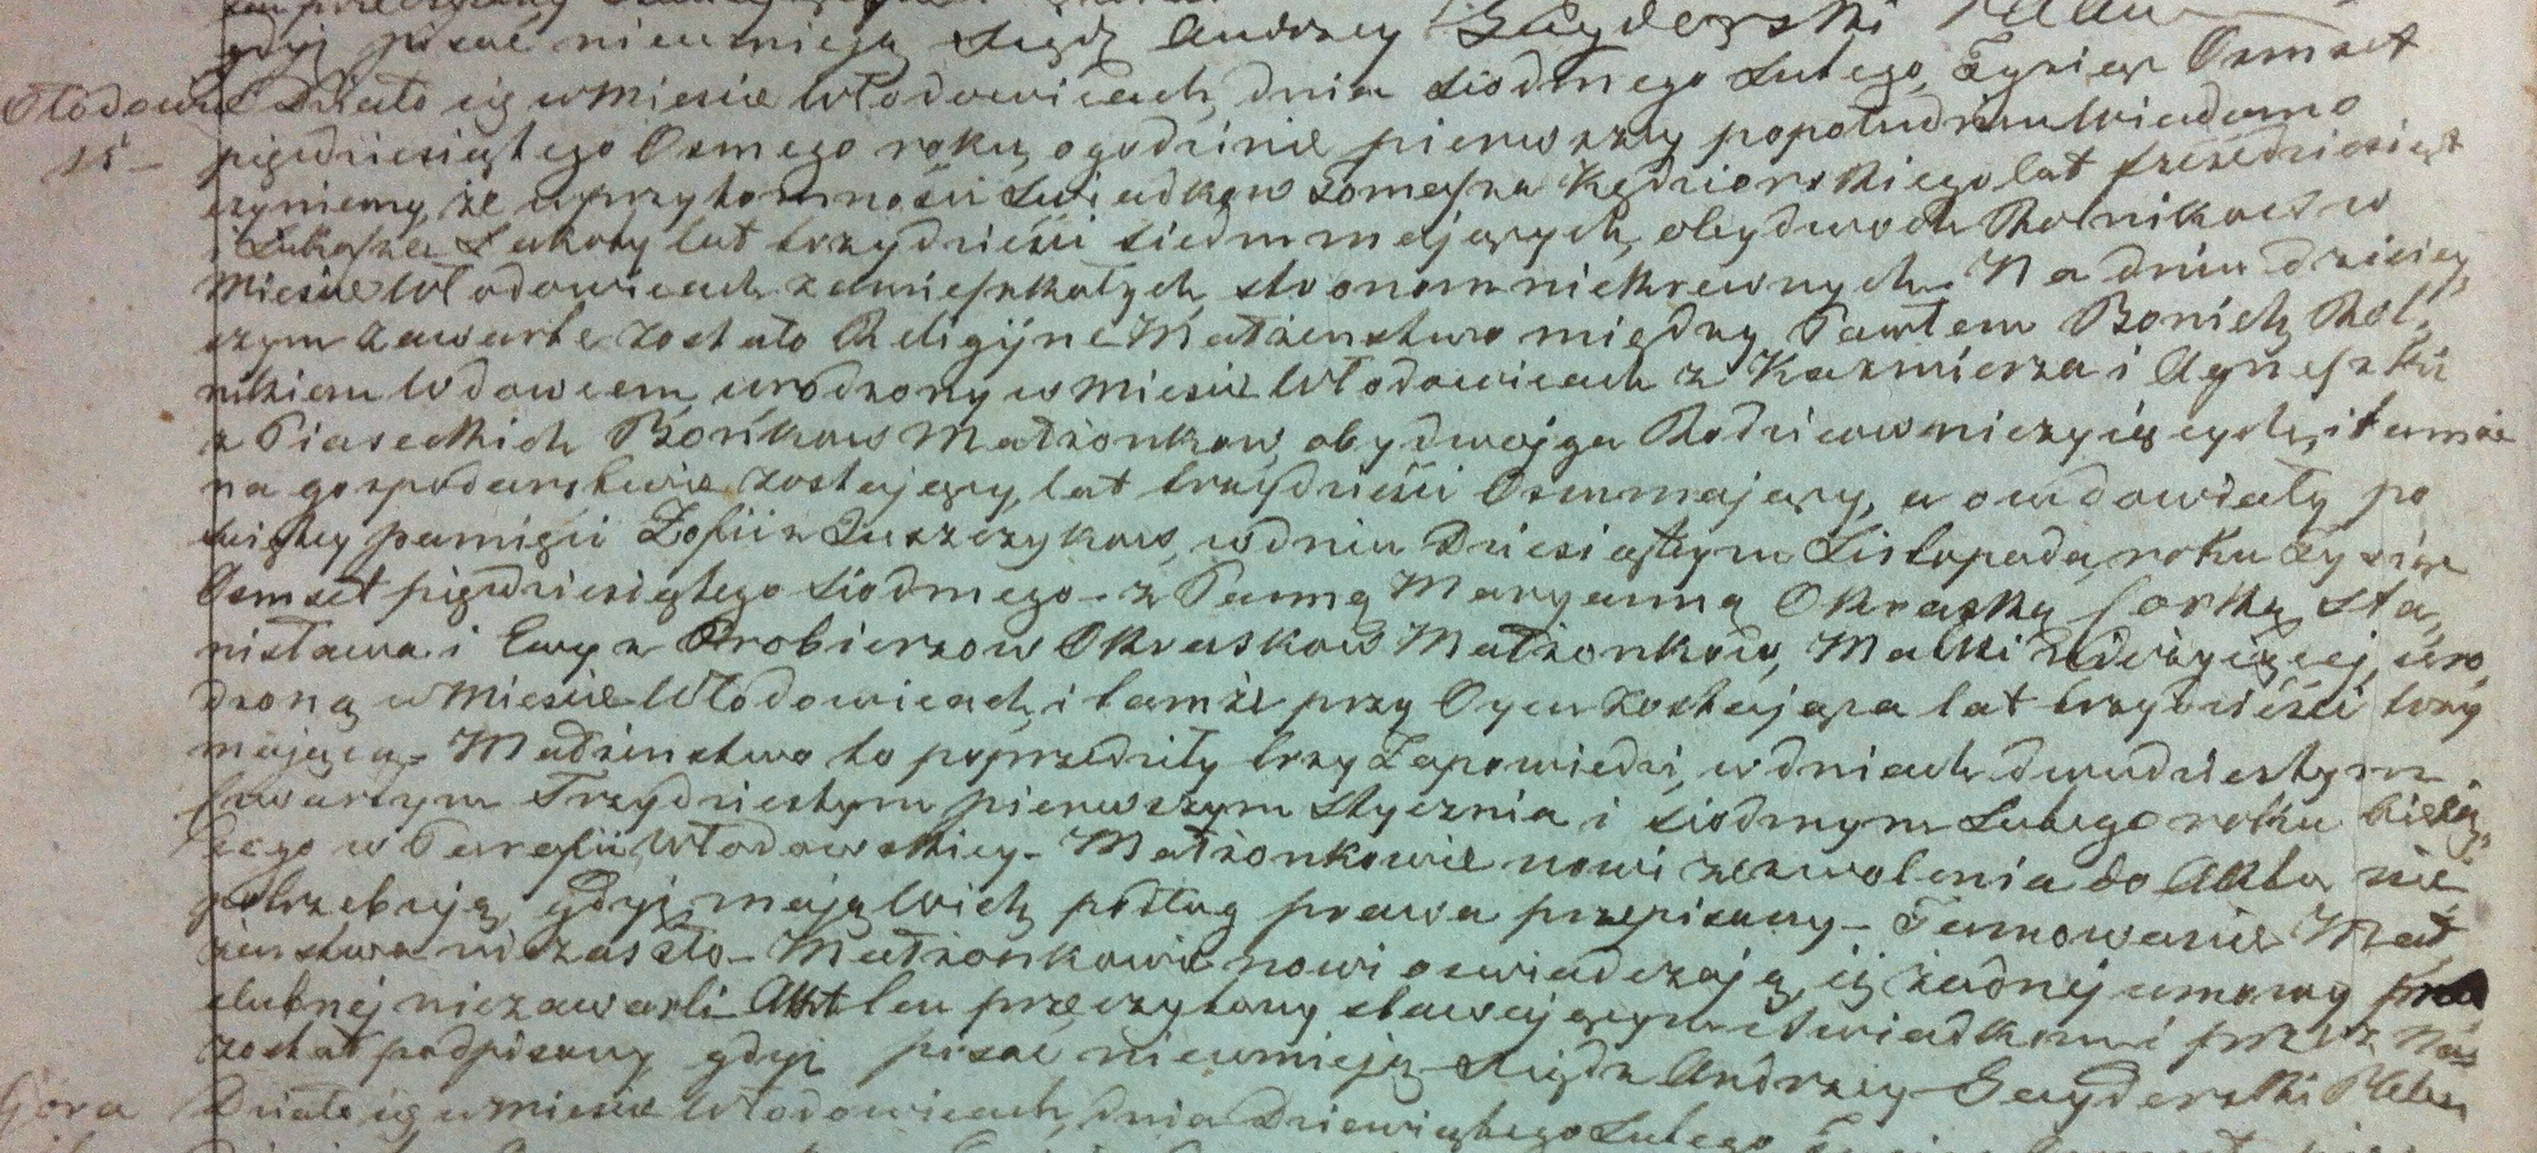
\includegraphics[width=0.8\textwidth]{zdjecia/akt_slubu_pawla_bonka_i_marianny_okraski.jpg}
\caption[Akt ślubu Pawła Bońka z Marianną Okraską]{Akt ślubu Pawła Bońka (dziadka Antoniny Głąb z domu Łyszczarz) i jego drugiej żony Marianny Okraski}
\label{rys:akt_slubu_pawla_bonka_i_marianny_okraski}
\end{center}
\end{figure}

Nie wiem kiedy zmarł Paweł Boniek, ale na pewno przed 1874 rokiem, skoro Jego córka Józefa w 1874~r. bierze ślub z Maciejem już jako zupełna sierota...
Paweł Boniek jest protoplastą dwóch rodzin: Macieja i Kaspra Łyszczarzów poprzez jego dwie córki z dwóch matek, warto więc zacytować akt jego urodzenia: \textit{7 stycznia 1820~r. stawił się w kościele we Włodowicach Kazimierz Boniek, lat 32 liczący rolnik, mieszczanin w mieście Włodowicach, przy ojcu swym zamieszkały i okazał nam dziecię płci męskiej, które urodziło się w domu ojca jego Woyciecha Bońka pod  nr 115 dnia tego samego o godz. 1 po północy, oświadczając, iż jest z niego i jego prawowitej małżonki  Piaseczczanki lat 28 mającej i że życzeniem jego jest nadać mu imię Paweł}.


%TODO ***zdj aktu ur. Pawła Bońka  nowy pdr. Nr }

Ów Paweł Boniek dwa razy się żenił. Najpierw 23 XI 1841~r. we Włodowicach w przytomności świadków […] zostało zawarte religijne małżeństwo między Pawłem Bońkiem -- młodzianem w mieście Włodowicach zamieszkałym i tamże urodzony z Kazimierza i Agnieszki z Piaseckich -- małżonków Bońków -- obydwóch rodziców żyjących i tamże przy rodzicach zostający, lat 21 i miesięcy 10 mający z panną Zofią Juszczykówną, córką Idziego i Elżbiety z Wcisłów -- małżonków Juszczyków, obydwóch rodziców nieżyjących, urodzoną w mieście Włodowicach i tamże w służbie zostającą, lat 20 i miesięcy ośm mająca. Zezwolenie na ślub jest od rodziców Pawła Bońka oraz od Rady Familijnej zdziałanej w Urzędzie Burmistrza Miasta Włodowice w dniu 20 XI 1841~r.

\begin{figure}[!h]
\begin{center}
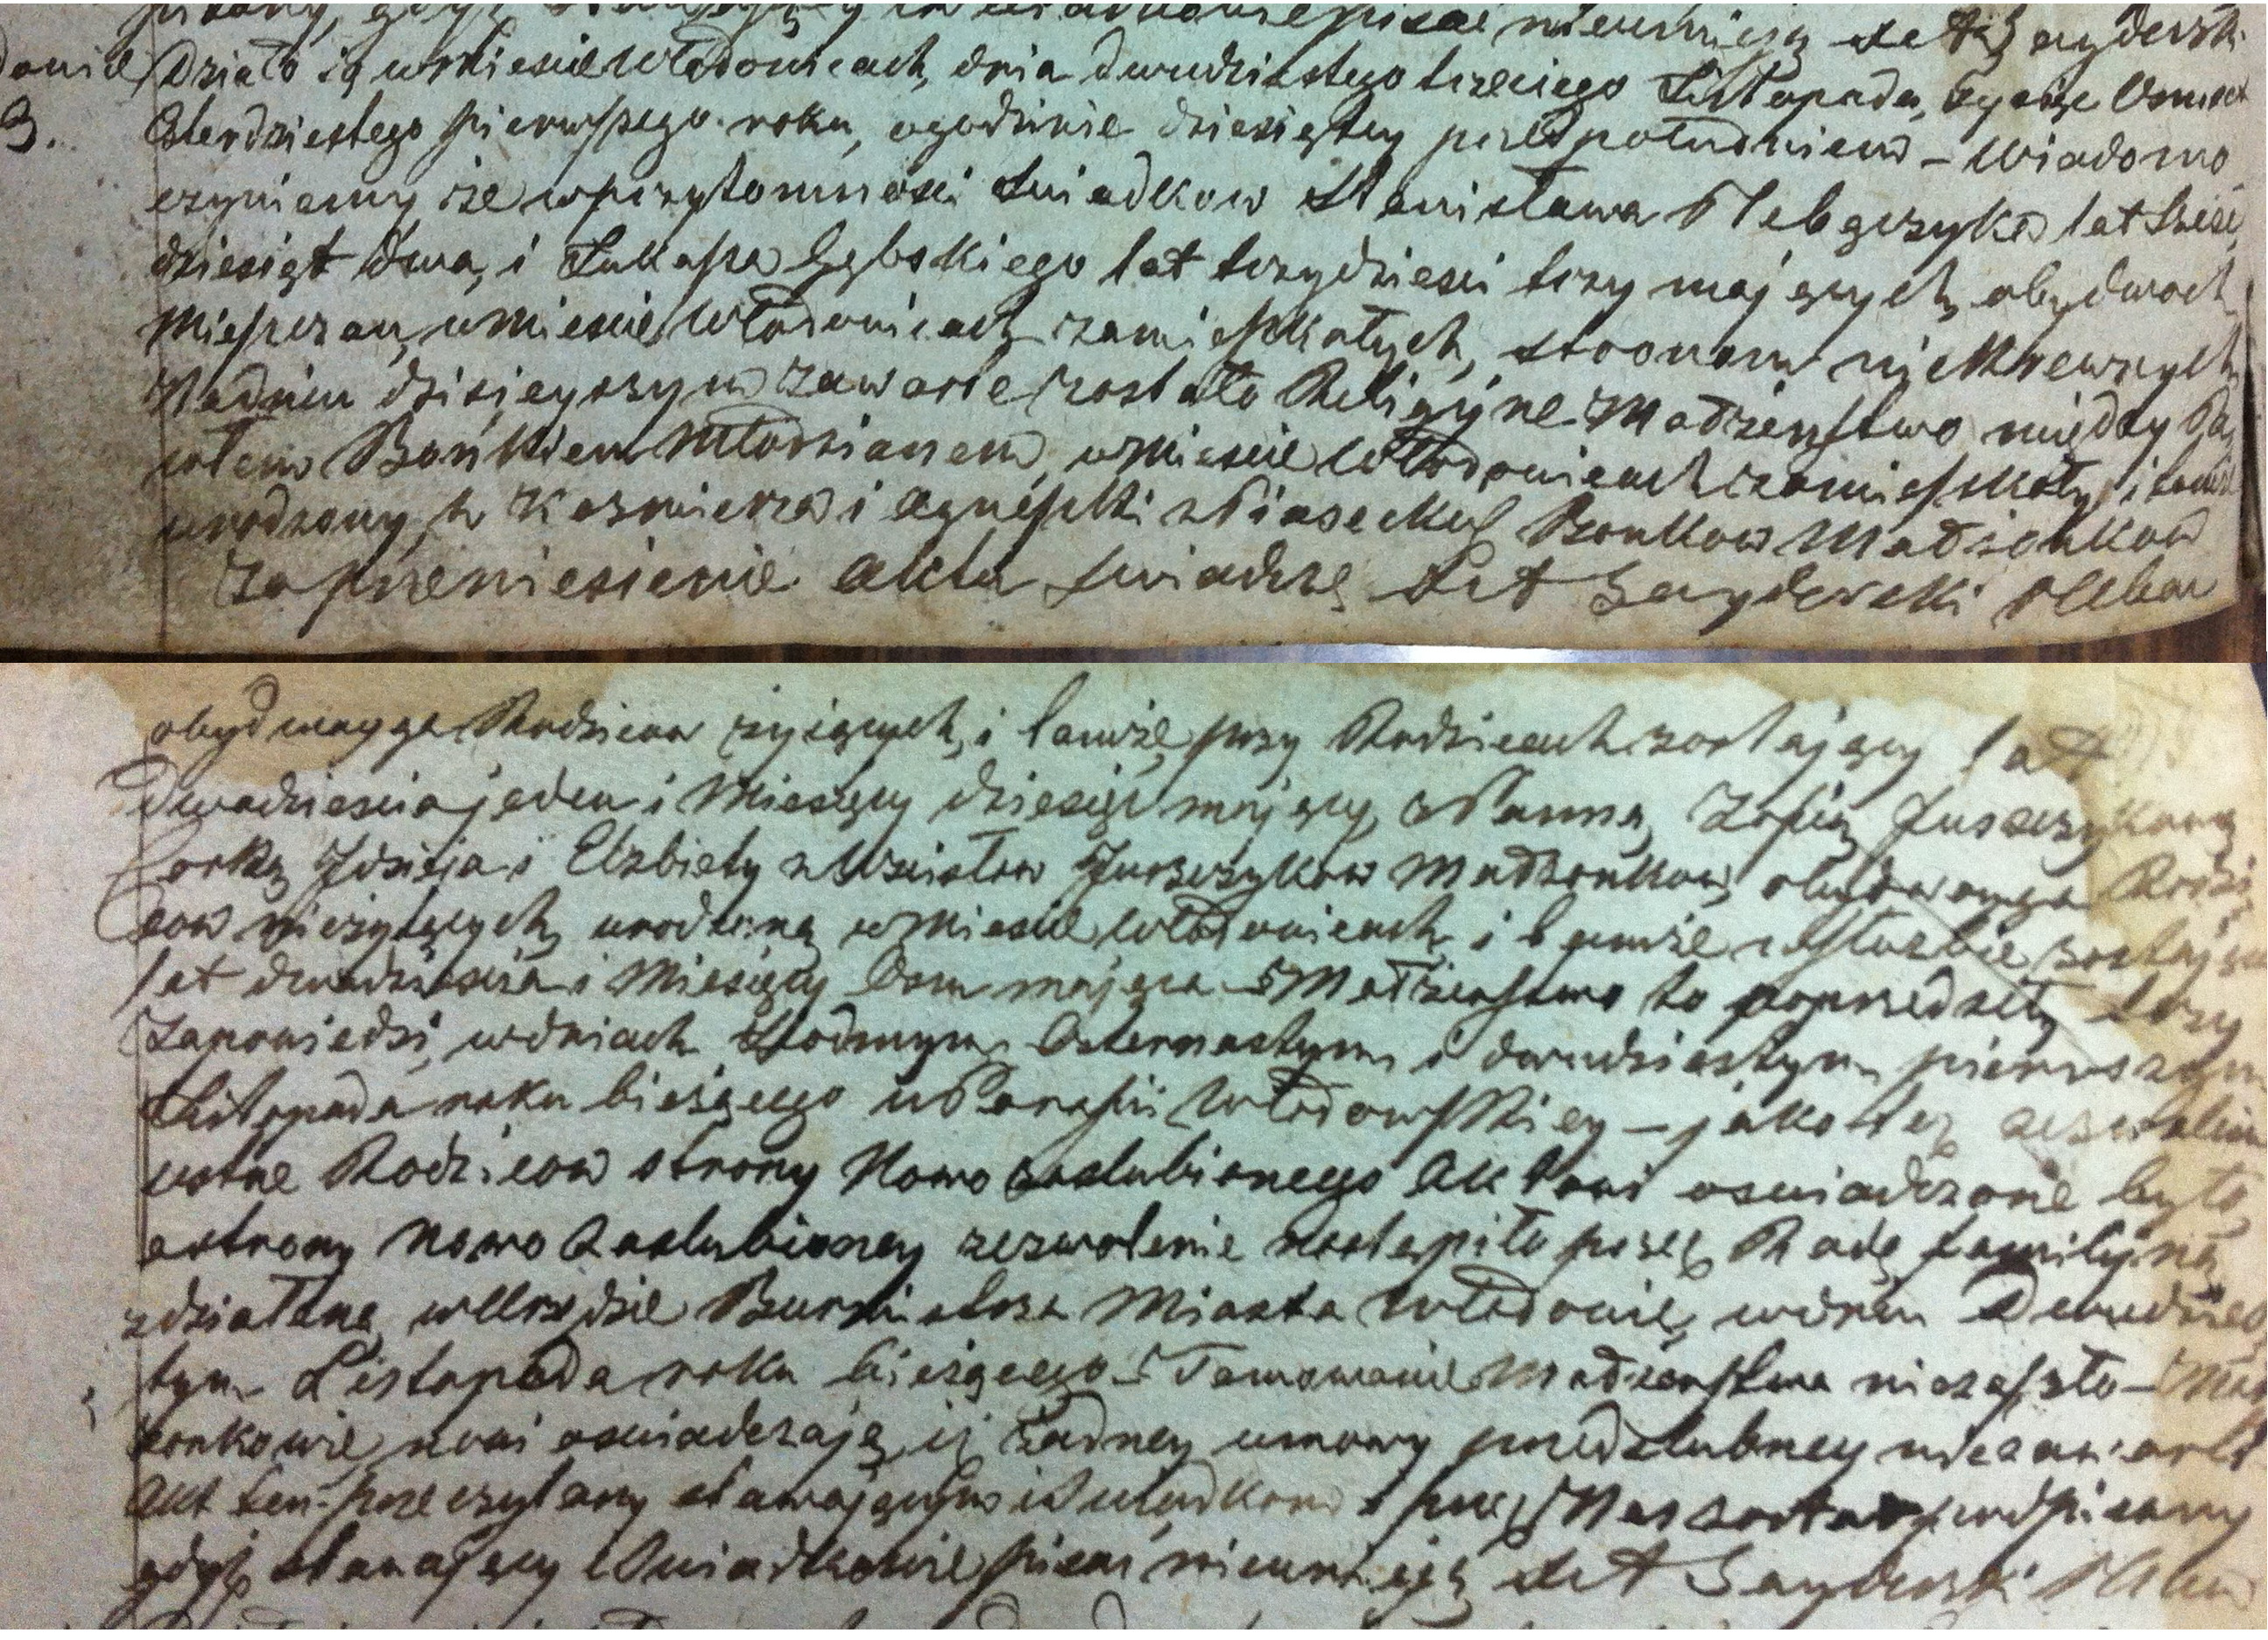
\includegraphics[width=0.8\textwidth]{zdjecia/akt_slubu_pawla_bonka_i_zofii_juszczyk.jpg}
\caption[Akt ślubu Pawła Bońka z Zofią Juszczyk]{Akt ślubu dziadków Antoniny Głąb z domu Łyszczarz: Pawła Bońka z Zofią Juszczyk}
\label{rys:akt_slubu_pawla_bonka_i_zofii_juszczyk}
\end{center}
\end{figure}

Z tego małżeństwa przyszła na świat m.in. Józefa Boniek, żona Macieja Łyszczarza a następnie Józefa Smolenia i matka Antoniny oraz Hilarego Łyszczarzów, a także Feliksa Smolenia z drugiego małżeństwa.

Drugi raz ożenił się Paweł Boniek 7 lutego 1858~r., gdy miał 38 lat, owdowiały po św. pamięci Zofii z Juszczyków zmarłej 10 XI 1857~r. Ożenił się z Marianną Okraską, córką Stanisława i Ewy z Dorobiszów – małżonków Okrasków, matki nieżyjącej, urodzoną w mieście Włodowicach i tamże przy ojcu zostającą, lat 33 mającą. 

Z tego małżeństwa przyszła na świat m.in. \textbf{Antonina Boniek}, która dnia \textbf{6 VII 1880~r.} we Włodowicach wyszła za \textbf{Kaspra Łyszczarza}. \textbf{Antonina Boniek zmarła 3 X 1929~r. w Górze Włodowskiej} czyniąc wdowcem swego męża Kaspra. \textbf{Kasper zmarł} w 7 lat po niej, tj. \textbf{6 IX 1936~r. w Górze}. Tak więc za zrządzeniem Boskim Antonina i Hilary Łyszczarze trafili pod dach brata swego ojca Macieja i siostry swej matki Józefy. Oto jeszcze jeden przykład, że Boża Opatrzność czuwa... Kasper Łyszczarz z Antoniną Boniek doczekali się sześciorga dzieci: córki Balbiny ur. 28 X 1881~r., syna Józefa Łyszczarza ur. 6 X 1888~r., córki Marianny Łyszczarz ur. 24 VI 1890~r., syna Antoniego Łyszczarza ur. 9 V 1893~r., córki Władysławy Łyszczarz ur. 23 V 1895~r. oraz córki Weroniki Łyszczarz ur. 16 XI 1899~r. Wszyscy urodzeni w Górze Włodowskiej. Najstarszy syn Kaspra -- Józef Łyszczarz dwa razy się żenił, najpierw 25 I 1921~r. z Józefą Dyrdoń, a następnie 8 X 1928~r. z Franciszką Morawską. Ich córka Władysława wyszła 16 X 1917~r. za Bolesława Mygę  z par. włodowickiej, a Weronika Łyszczarz wyszła 16 XI 1927~r. za Franciszka Pakułę. Natomiast ich córka Marianna zmarła w wieku 14 lat, tj. 1 VII 1904~r. we wsi Góra.

Natomiast Walenty Głąb miał więcej szczęścia, gdyż przy jego ślubie byli oboje rodzice. Walenty Głąb urodził się 10 lutego 1869~r. w Mirowie z Macieja lat 30 i Marianny z domu Hamerla też lat 30. Rodzicami chrzestnymi byli Jan Górski i Marianna Radosz.

\begin{figure}[!h]
\begin{center}
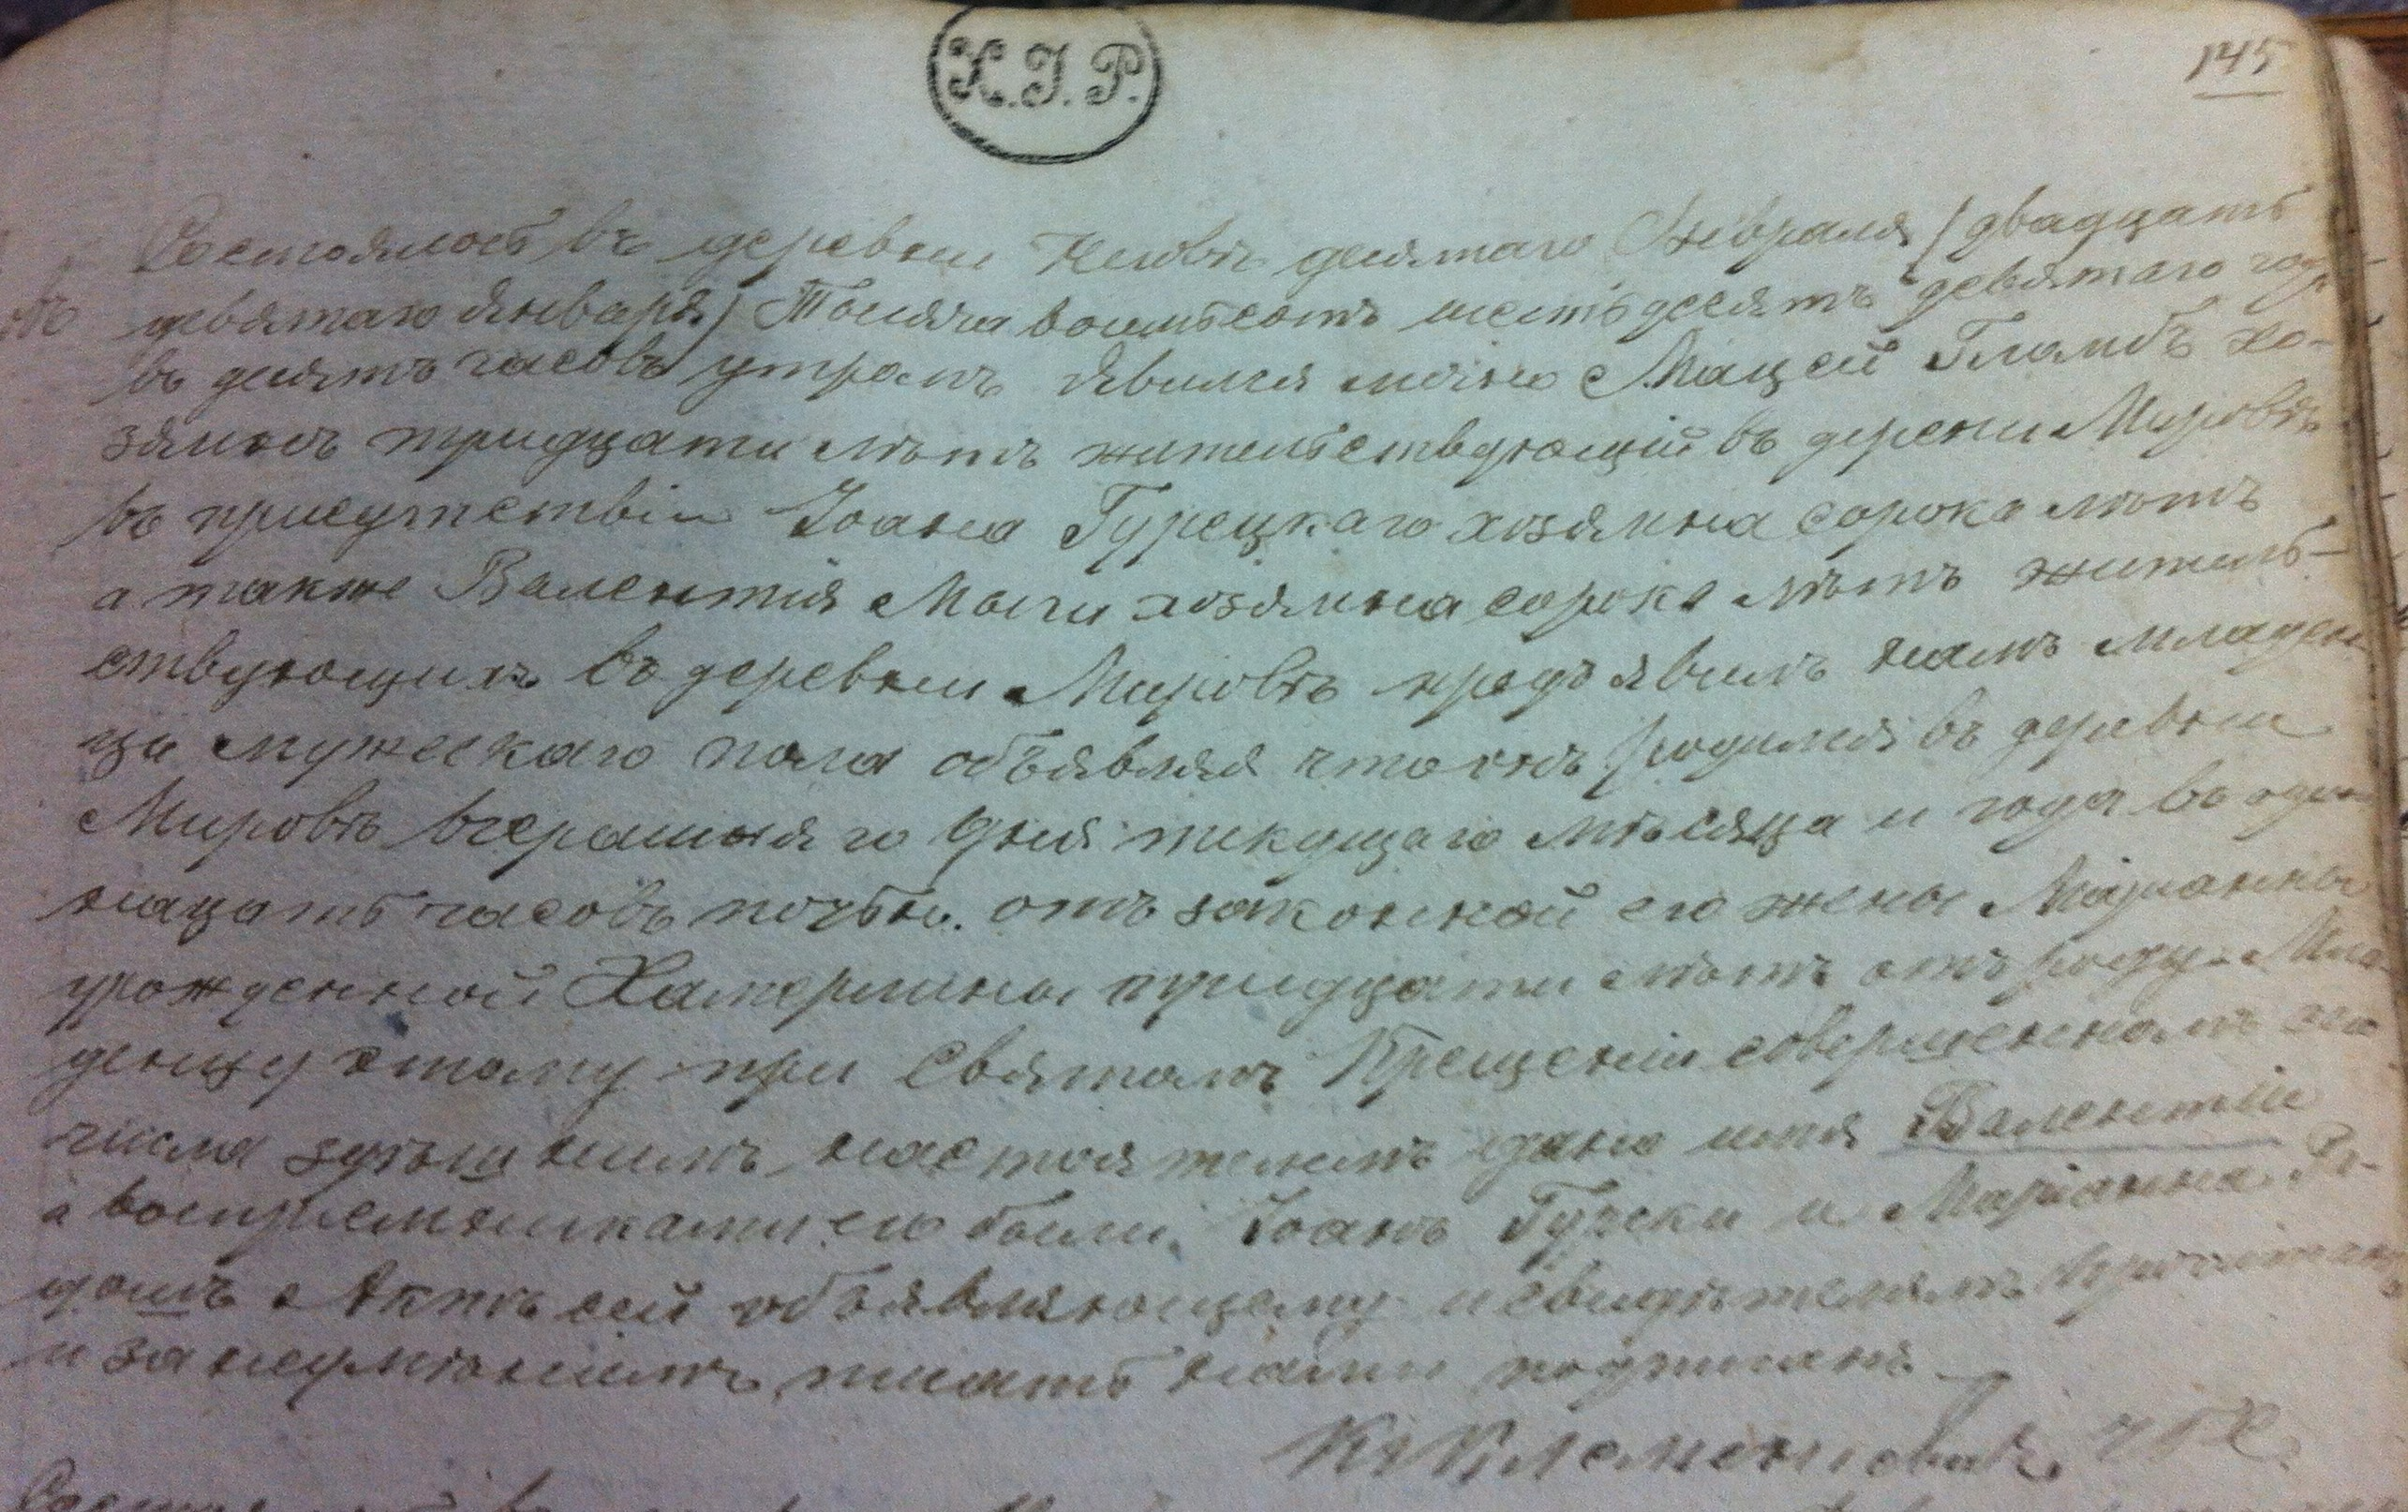
\includegraphics[width=0.8\textwidth]{zdjecia/akt_urodzenia_walentego_glaba.jpg}
\caption[Akt urodzenia Walentego Głąba]{Akt urodzenia Walentego Głąba, syna Macieja i Marianny z domu Hamerla}
\label{rys:akt_urodzenia_walentego_glaba}
\end{center}
\end{figure}

Akt ślubu rodziców Walentego sporządzony jest po polsku, gdyż  ślub ich odbył się jeszcze przed represjami jakie miały miejsce po Powstaniu Styczniowym. Na stronie 222 pod nr 24 sporządzony jest następujący akt ślubu: Działo się w Niegowie dnia 14 listopada 1853~r. o godzinie dwunastej w południe. Wiadomo czyniemy, iż w przytomności świadków Jakuba Lamcha, lat 50 i Walentego Pawuli lat 42 mających, obydwóch zagrodników we wsi Ogorzelniku zamieszkałych na dniu dzisiejszym zawarte zostało religijne małżeństwo między Maciejem Głąbem, młodzianem lat dwadzieścia mającym, synem Szymona i Marianny z Bialików – małżonków Głąbów, włościan we wsi Mirowie w Parafii tutejszej urodzonym i tamże przy rodzicach zostającym, a Maryanną Hamerlanką, panną, lat osiemnaście ukończonych mającą, córką Jana i Marianny z Cyzów, małżonków Hamerlów we wsi Ogorzelniku w parafii tutejszej urodzoną i tamże przy rodzicach zostającą. Małżeństwo to poprzedziły trzy zapowiedzi. Małżonkowie nowi oświadczają, iż nie zawarli z sobą żadnej umowy przedślubnej. Obecni rodzice nowozaślubionych ustnie na ten akt zezwolili. Po czem akt ten stawającym i świadkom został przeczytany, przez nas samych podpisany, gdyż ci pisać nie umieją. Podpisał ksiądz Jan Markowski.

\begin{figure}[!h]
\begin{center}
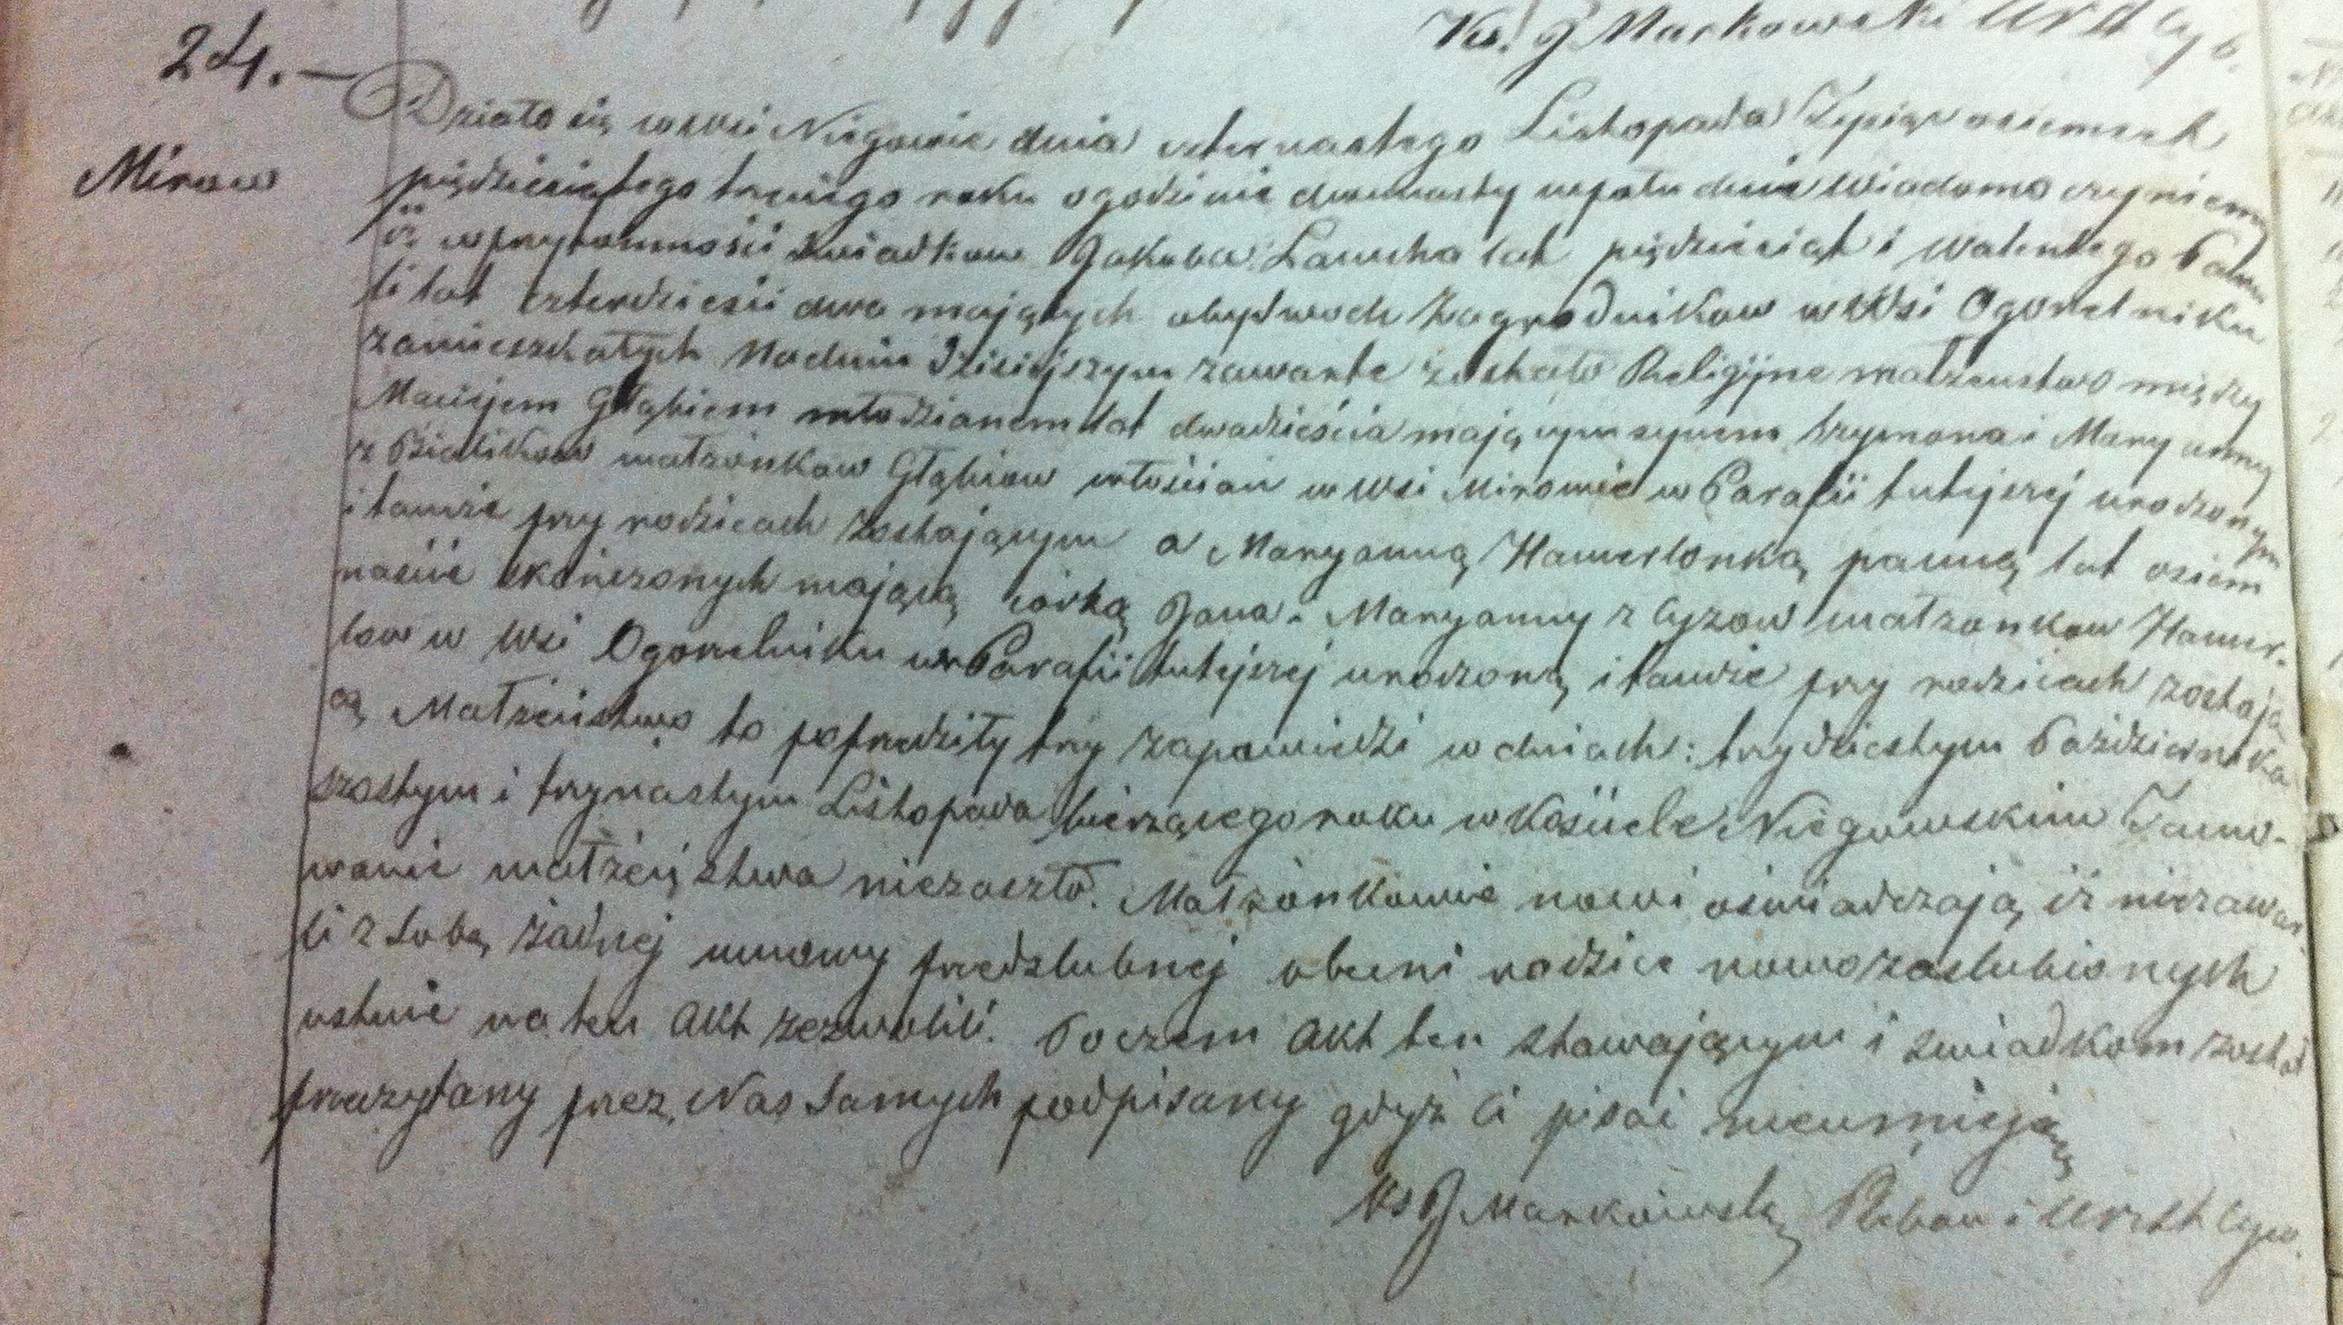
\includegraphics[width=0.8\textwidth]{zdjecia/akt_slubu_macieja_glaba_i_marianny_hamerli.jpg}
\caption[Akt ślubu Macieja Głąba z Marianną Hamerlą]{Akt ślubu Macieja Głąba i Marianny Hamerla -- rodziców Walentego}
\label{rys:akt_slubu_macieja_glaba_i_marianny_hamerli}
\end{center}
\end{figure}

Akt urodzenia Macieja Głąba zapisany na str. 184 pod nr 13 Księgi urodzeń parafii Niegowa tak oto się przedstawia: Działo się we wsi Niegowej roku 1833 dnia 22 lutego o godzinie pierwszej po południu stawił się Szymon Głąb katolik liczący lat 31 włościanin w Mirowie zamieszkały w przytomności świadków Wincentego Zielińskiego i Michała Palucha obydwóch czterdziestoletnich w Mirowie zamieszkałych i okazał nam dziecię płci męskiej urodzone w domu jego pod numerem czwartym na dniu 21 lutego o godzinie pierwszej po południu oświadczając, że jest z niego i Marianny z Białów – żony jego katoliczki liczącej lat 30 spłodzone. Dziecięciu temu na chrzcie świętym na dniu dzisiejszym odbytym nadano imię Maciej, a rodzicami chrzestnymi byli Wincenty Zieliński i Teresa Pilisowa.

\begin{figure}[!h]
\begin{center}
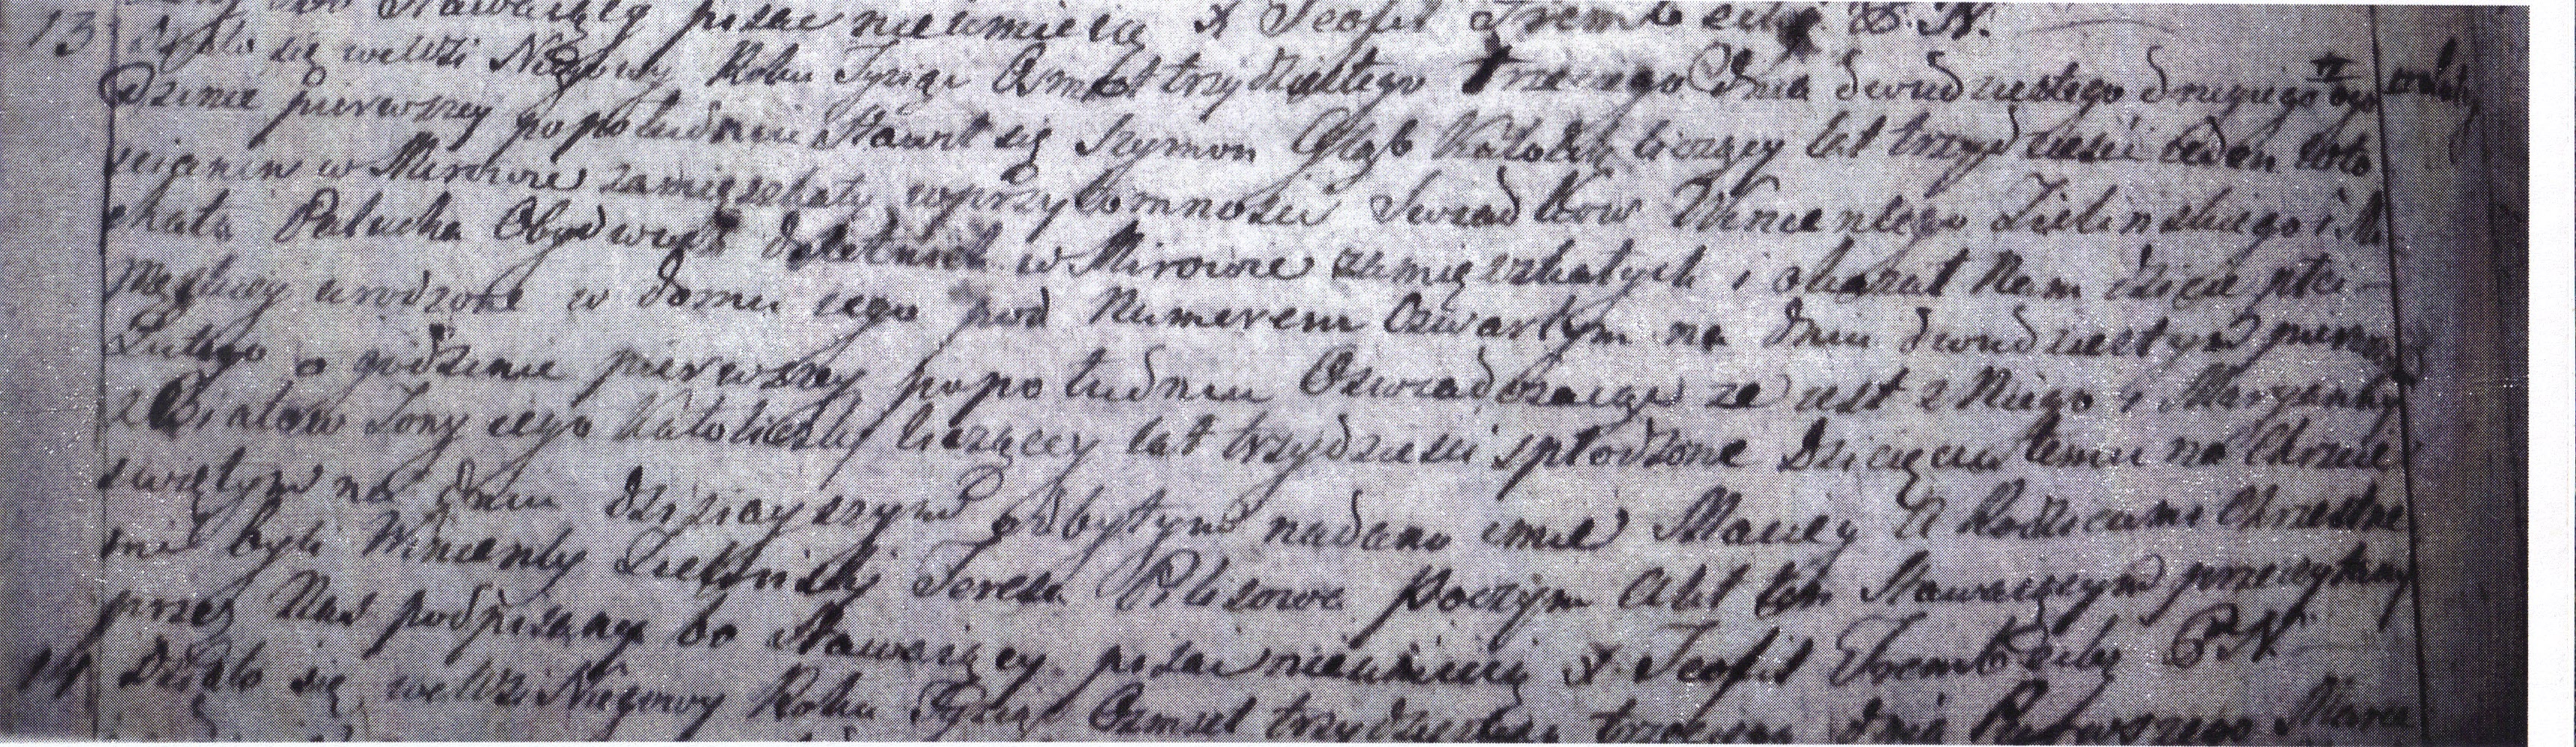
\includegraphics[width=0.8\textwidth]{zdjecia/akt_urodzenia_macieja_glaba.jpg}
\caption[Akt urodzenia Macieja Głąba]{Akt urodzenia Macieja Głąba - syna Szymona i Marianny Bialik}
\label{rys:akt_urodzenia_macieja_glaba}
\end{center}
\end{figure}

Rodzice przyszłej żony Macieja Głąba -- Marianny Chamerli pobrali się w mieście Włodowicach dnia 25 VI 1827~r. o 8 rano w przytomności świadków -- Józefa Janoszki -- rolnika z Kotowic, tamże zamieszkałego, lat 45 i Bartłomieja Labochy -- rolnika w Kotowicach zamieszkałego, lat 50 mającego, niekrewnych. Zawarte wówczas zostało religijne małżeństwo między Janem Chamerlą -- wdowcem, rolnikiem w Ogorzelniku zamieszkałym, urodzonym we wsi Ogorzelniku z Benedykta i Heleny małżonków Chamerlów tamże zamieszkałych, już zmarłych, lat 46 mającym, a panną Marcyanną, córką Kazimierza i Zofii -- małżonków Czyżów w Kotowicach zamieszkałych, lat 19 liczącą, w Kotowicach zrodzoną i przy rodzicach zostającą.

\begin{figure}[!h]
\begin{center}
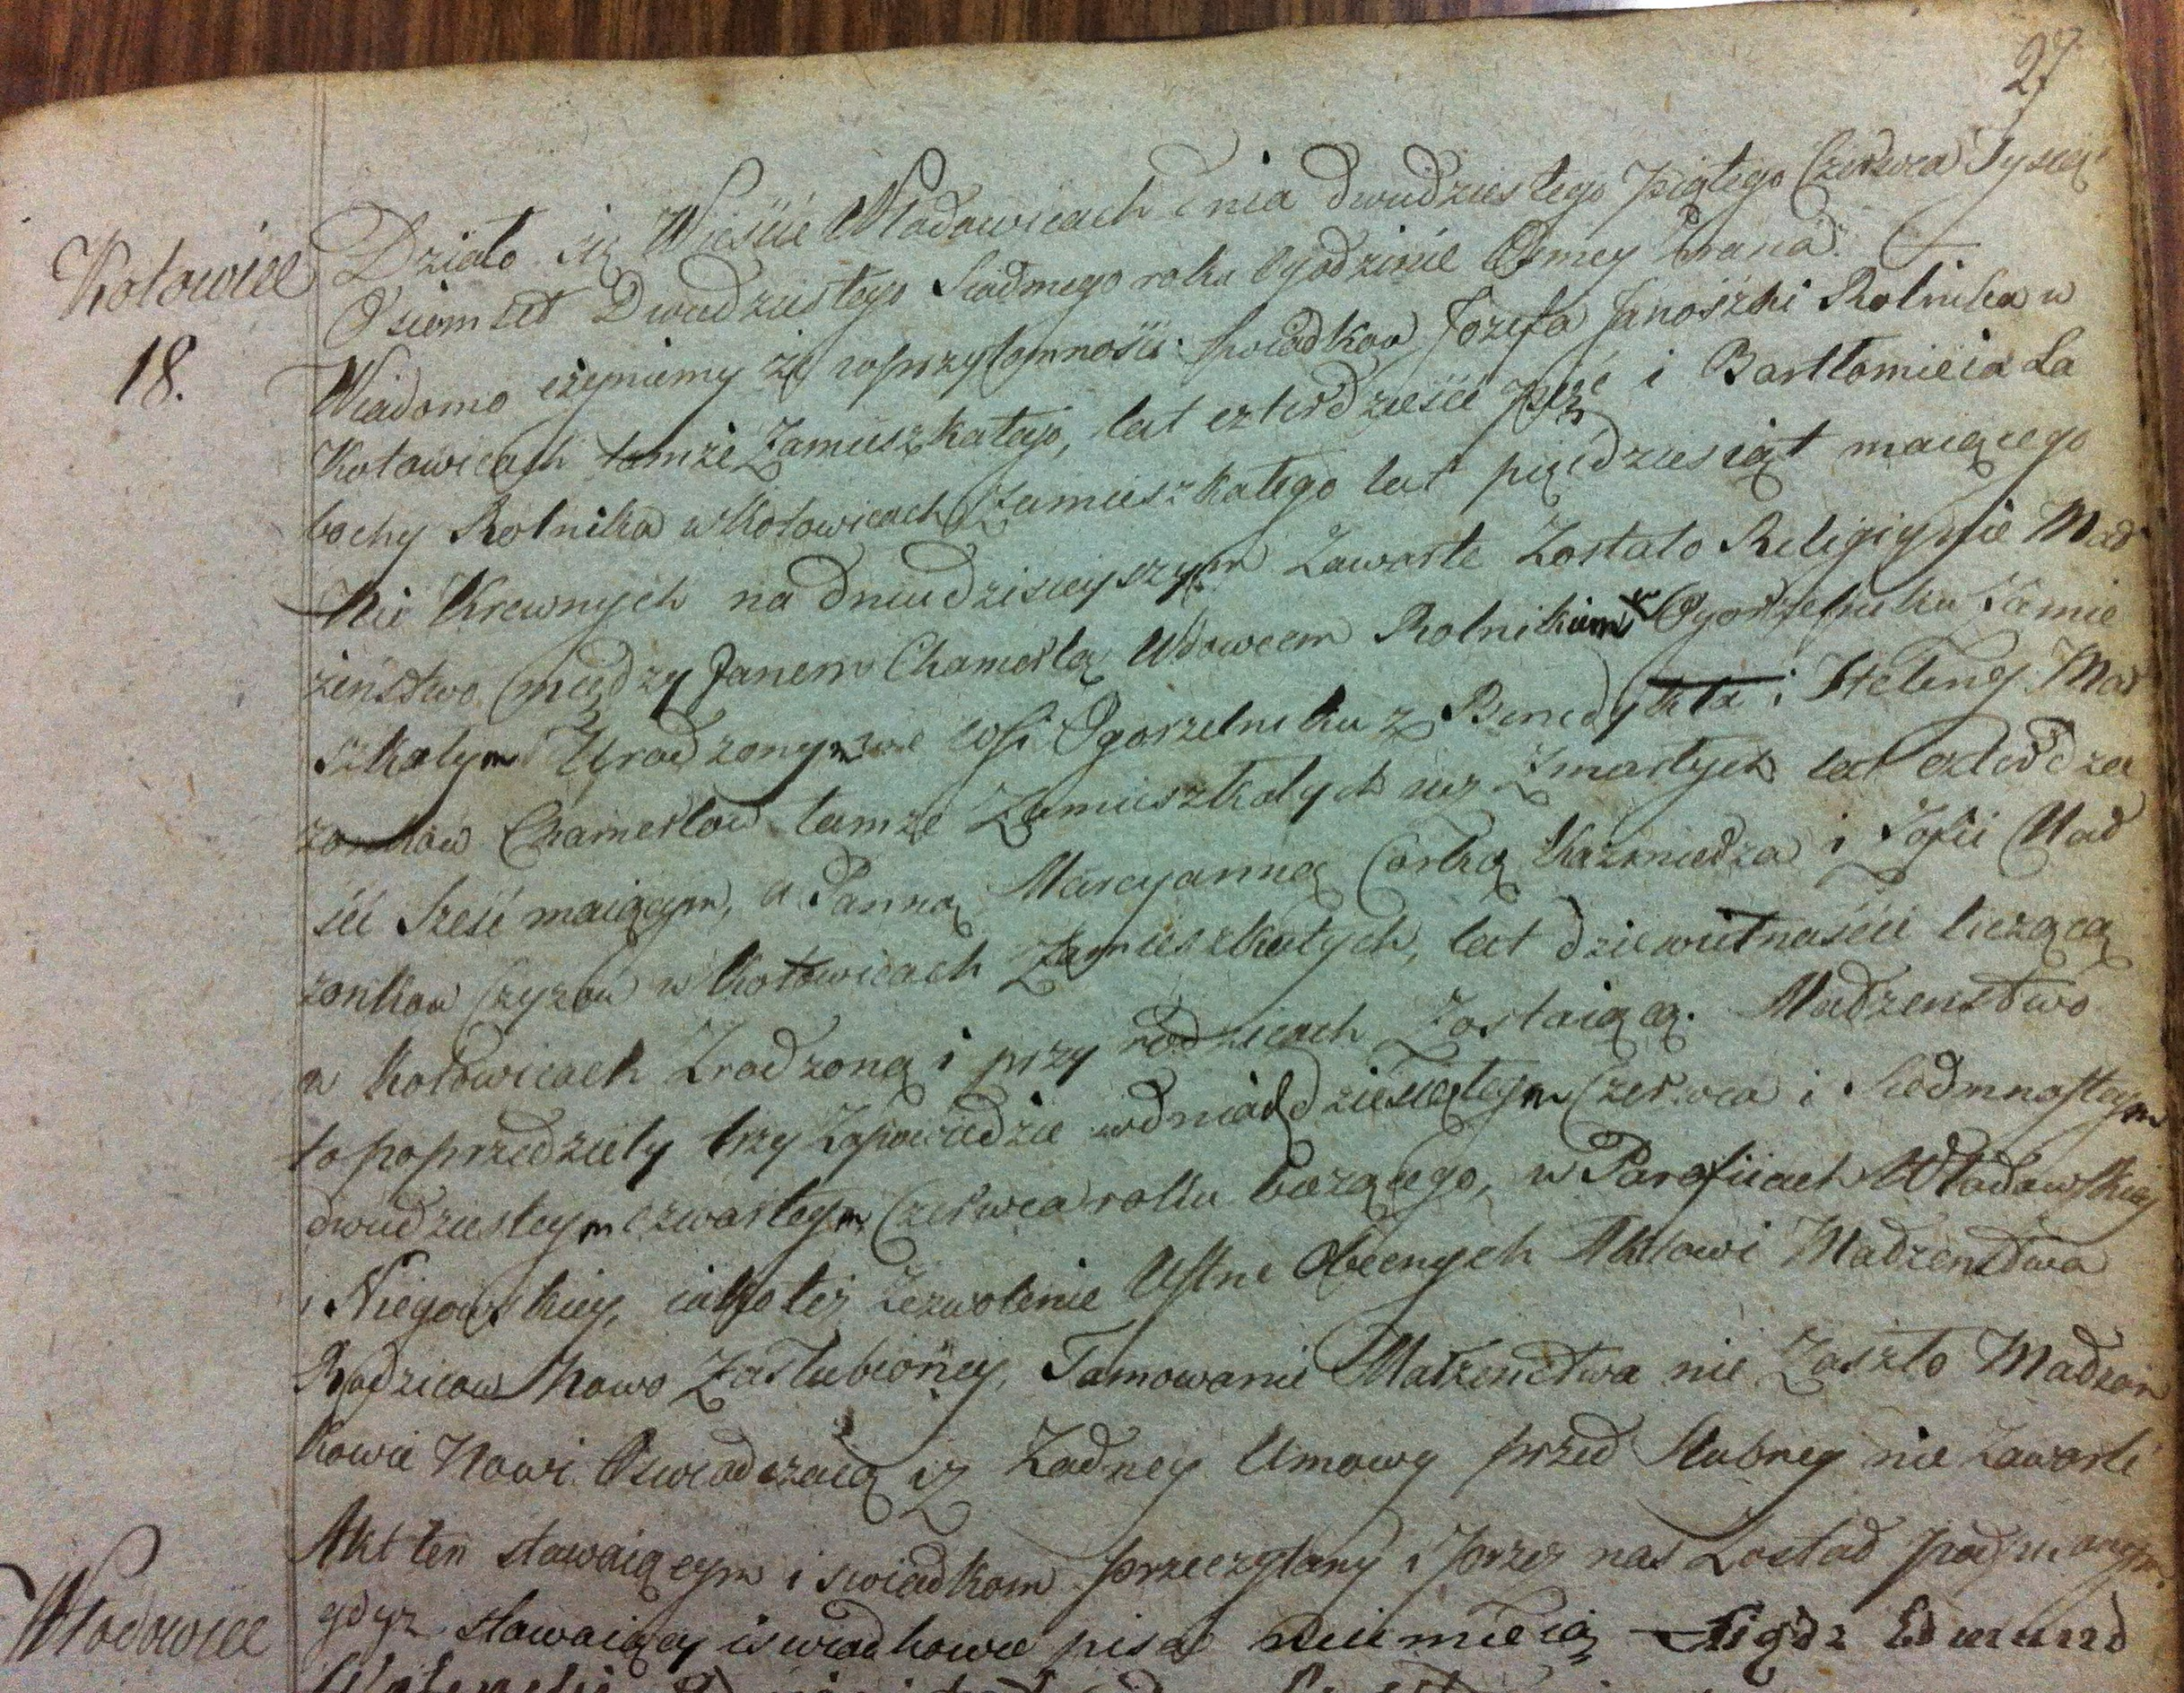
\includegraphics[width=0.7\textwidth]{zdjecia/akt_slubu_jana_chamerli_i_marcjanny_czyz.jpg}
\caption[Akt ślubu Jana Chamerli z Marcjanną Czyż]{Akt ślubu Jana Chamerli z Marcjanną Czyż -- dziadków Walentego Głąba}
\label{rys:akt_slubu_jana_chamerli_i_marcjanny_czyz}
\end{center}
\end{figure}

Jan Chamerla był wdowcem po Magdalenie Wasiakównej, która zmarła 4 II 1827~r. w Ogorzelniku.
Akt urodzenia matki Walentego zawarty w tej samej księdze również zaczyna się od słów: ,,Działo się'' w Niegowie roku tysiąc ośmset trzydziestego szóstego dnia 31 lipca stawił się Jan Chamerla, zagrodnik, katolik liczący lat 49 zamieszkały w Ogorzelniku w przytomności Jana Lipskiego liczącego lat 52 i Jana Głąba liczącego lat 40 zamieszkałych w Ogorzelniku i okazał dziecię płci żeńskiej urodzone w domu jego pod numerem dwunastym dnia 30 lipca o godzinie jedynastej przed południem oświadczający, że jest z niego i Marianny z Cyzów katoliczki liczącej lat 30 żony jego spłodzone. Dziecięciu temu na chrzcie świętym na dniu dzisiejszym odbytym nadano imię Marianna, a rodzicami chrzestnymi byli Jan Morawiec i Katarzyna Chamerlowa.

\begin{figure}[!h]
\begin{center}
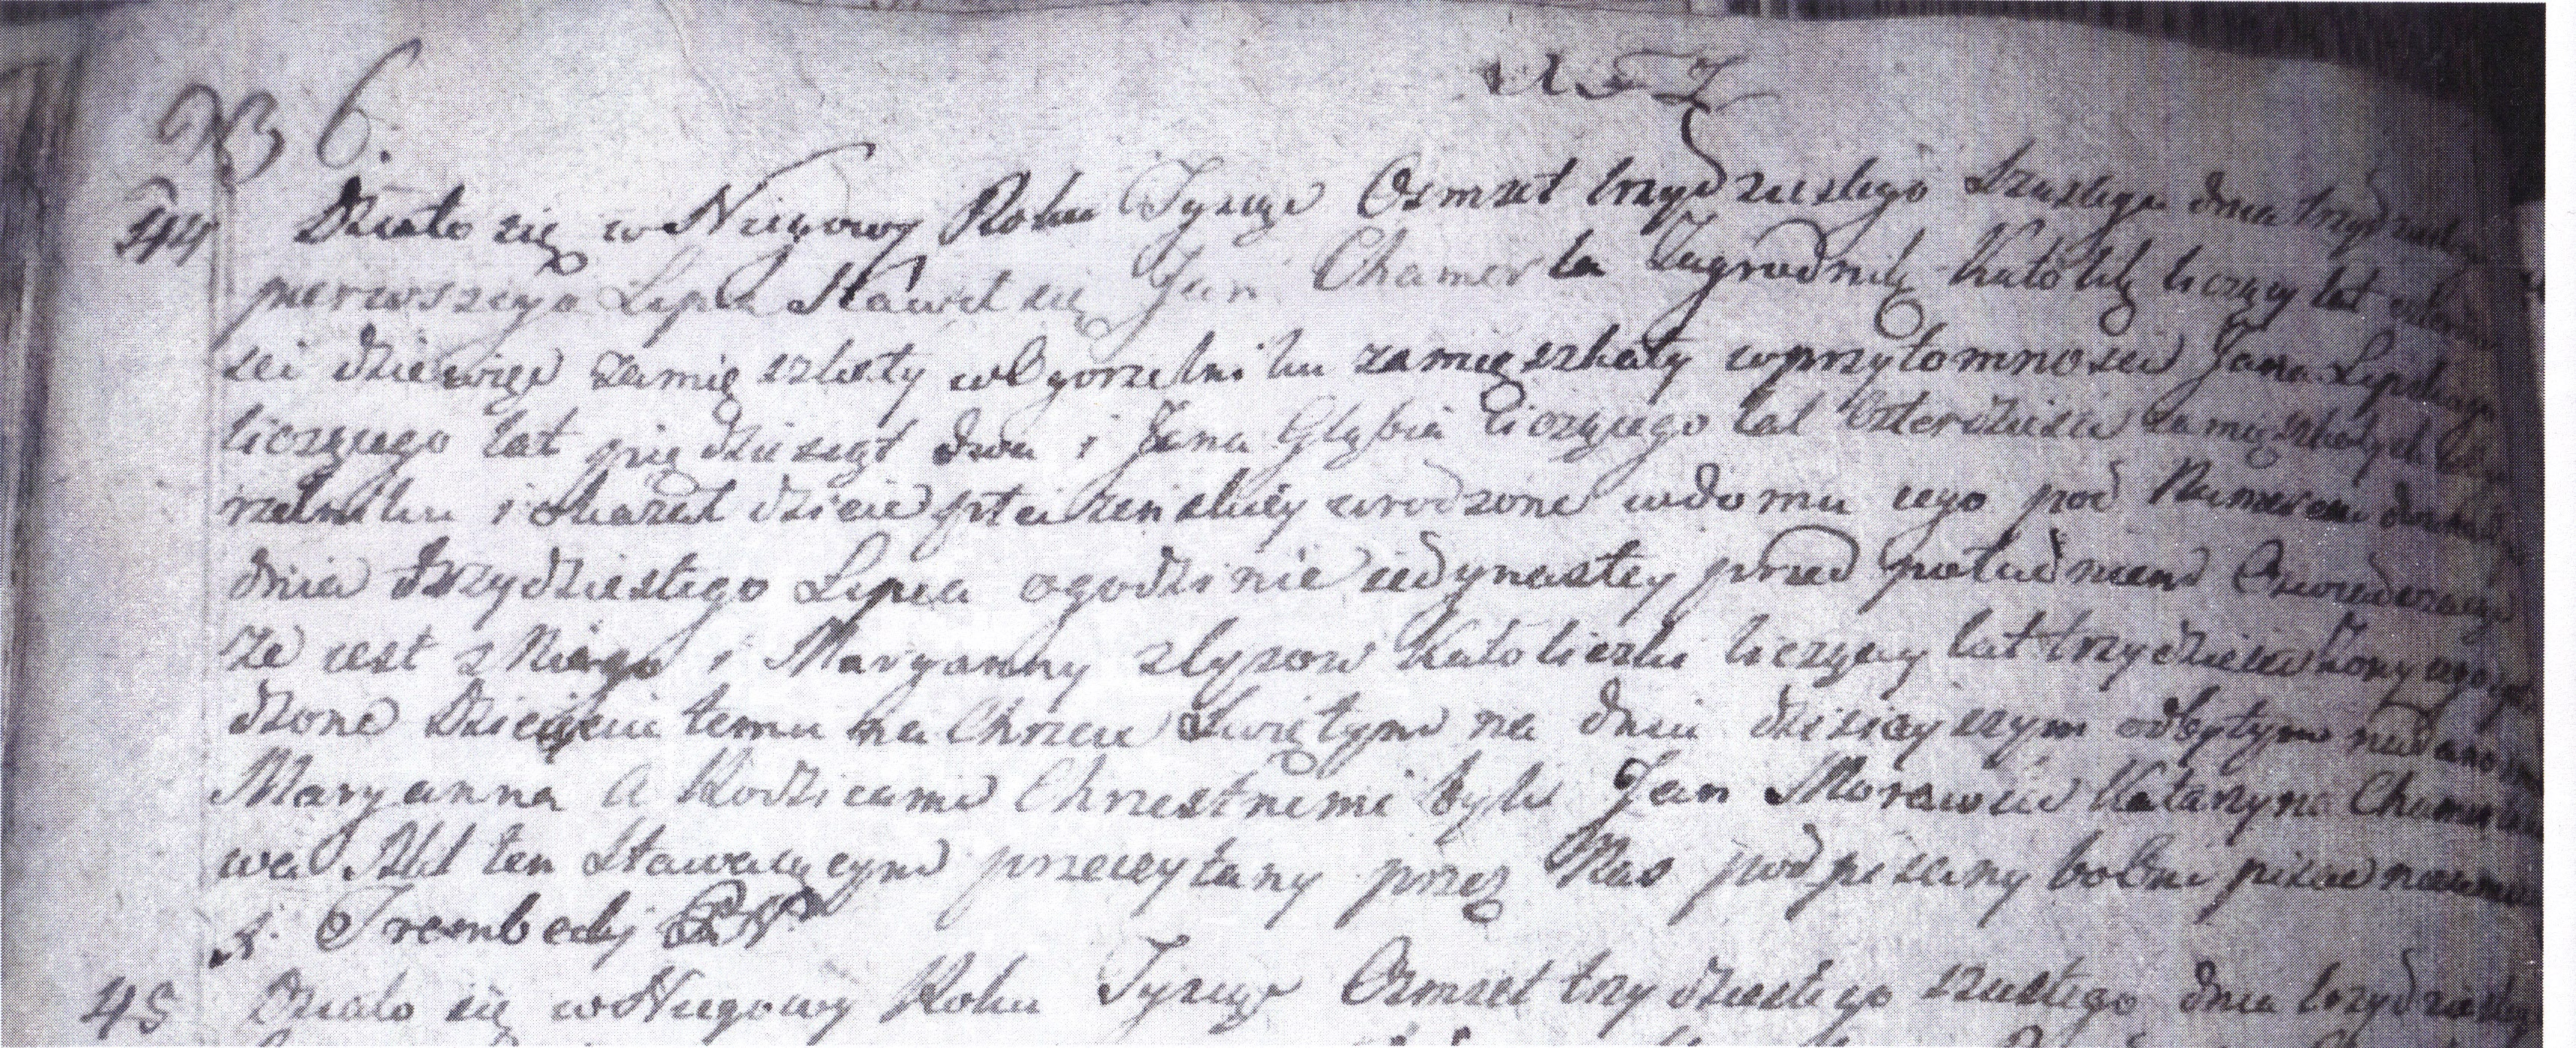
\includegraphics[width=0.8\textwidth]{zdjecia/akt_urodzenia_marianny_hamerla.jpg}
\caption[Akt urodzenia Marianny Hamerla]{Akt urodzenia Marianny Hamerla -- matki Walentego Głąba}
\label{rys:akt_urodzenia_marianny_hamerla}
\end{center}
\end{figure}

Badałem stan rodziny Macieja Głąba poprzez sporządzenie wypisu urodzeń Dzieci Macieja Głąba i jego małżonki Marianny z Chamerlów. Tych dzieci na przestrzeni 20 lat niewiele się pojawiło. Pierwszym był Mikołaj Głąb ur. 3 XII 1855~r. w Mirowie. Wówczas Maciej miał 21 lat a Marianna 20 lat. Rodzicami chrzestnymi byli Paweł Radosz i Helena Głąbowa. Kolejne ich dziecię -- Marianna Głąbówna -- jest zapisane w księdze metrykalnej dopiero w 1861~r. Ale krążący w rodzinie Walentego Głąba wierszyk zachowywał pamięć o trójce dzieci: ,,Malowane dzieci: Antosia, Sobosek, i Walosek trzeci''. Ale w niegowskiej księdze metrykalnej tylko Walosek, tj. Walenty Głąb jest zapisany w języku rosyjskim pod datą 28 stycznia (wg kalendarza juliańskiego) i 9 lutego według naszego, gregoriańskiego kalendarza. Jest to akt urodzenia i chrztu Walentego, a chrzestnymi byli Jan Górecki i Marianna Radosz.

Sebastian urodzony dziesięć lat wcześniej nie jest stricte zapisany w księdze metrykalnej, lecz jedynie na końcu alfabetycznego spisu aktów urodzeń za rok 1859 jest na str. 224 tej księgi pod ostatnim nazwiskiem urodzonego dziecięcia, tj. Wojtyli Andrzeja adnotacja tej treści: Głąb Sobestyan 12 - sty syn Macieja i Marianny z Hamerlów. Jest natomiast zachowany akt ślubu Sebastiana Głąba z Zuzanną Jawurą, który w tłumaczeniu z języka rosyjskiego tu przytaczam: Wydarzyło się 21 XI 1881~r. o 12 w południe, kiedy w obecności świadków [...] zawarto tego czasu religijny związek małżeński między Sobestianem (tak to imię jest tam zapisane) Głąbem, 22-letnim młodzianem, rolnikiem, synem Macieja i Marianny z Chamerlów -- małżonków Głąbów, urodzonym i zamieszkałym we wsi Mirów przy swoich rodzicach a Zuzanną Jawurą -- 22-letnią panną, córką Tadeusza i Marianny z Fronczków -- małżonków Jawurów -- rolników, urodzona i mieszkająca we wsi Moczydła przy swoich rodzicach.

\begin{figure}[!h]
\begin{center}
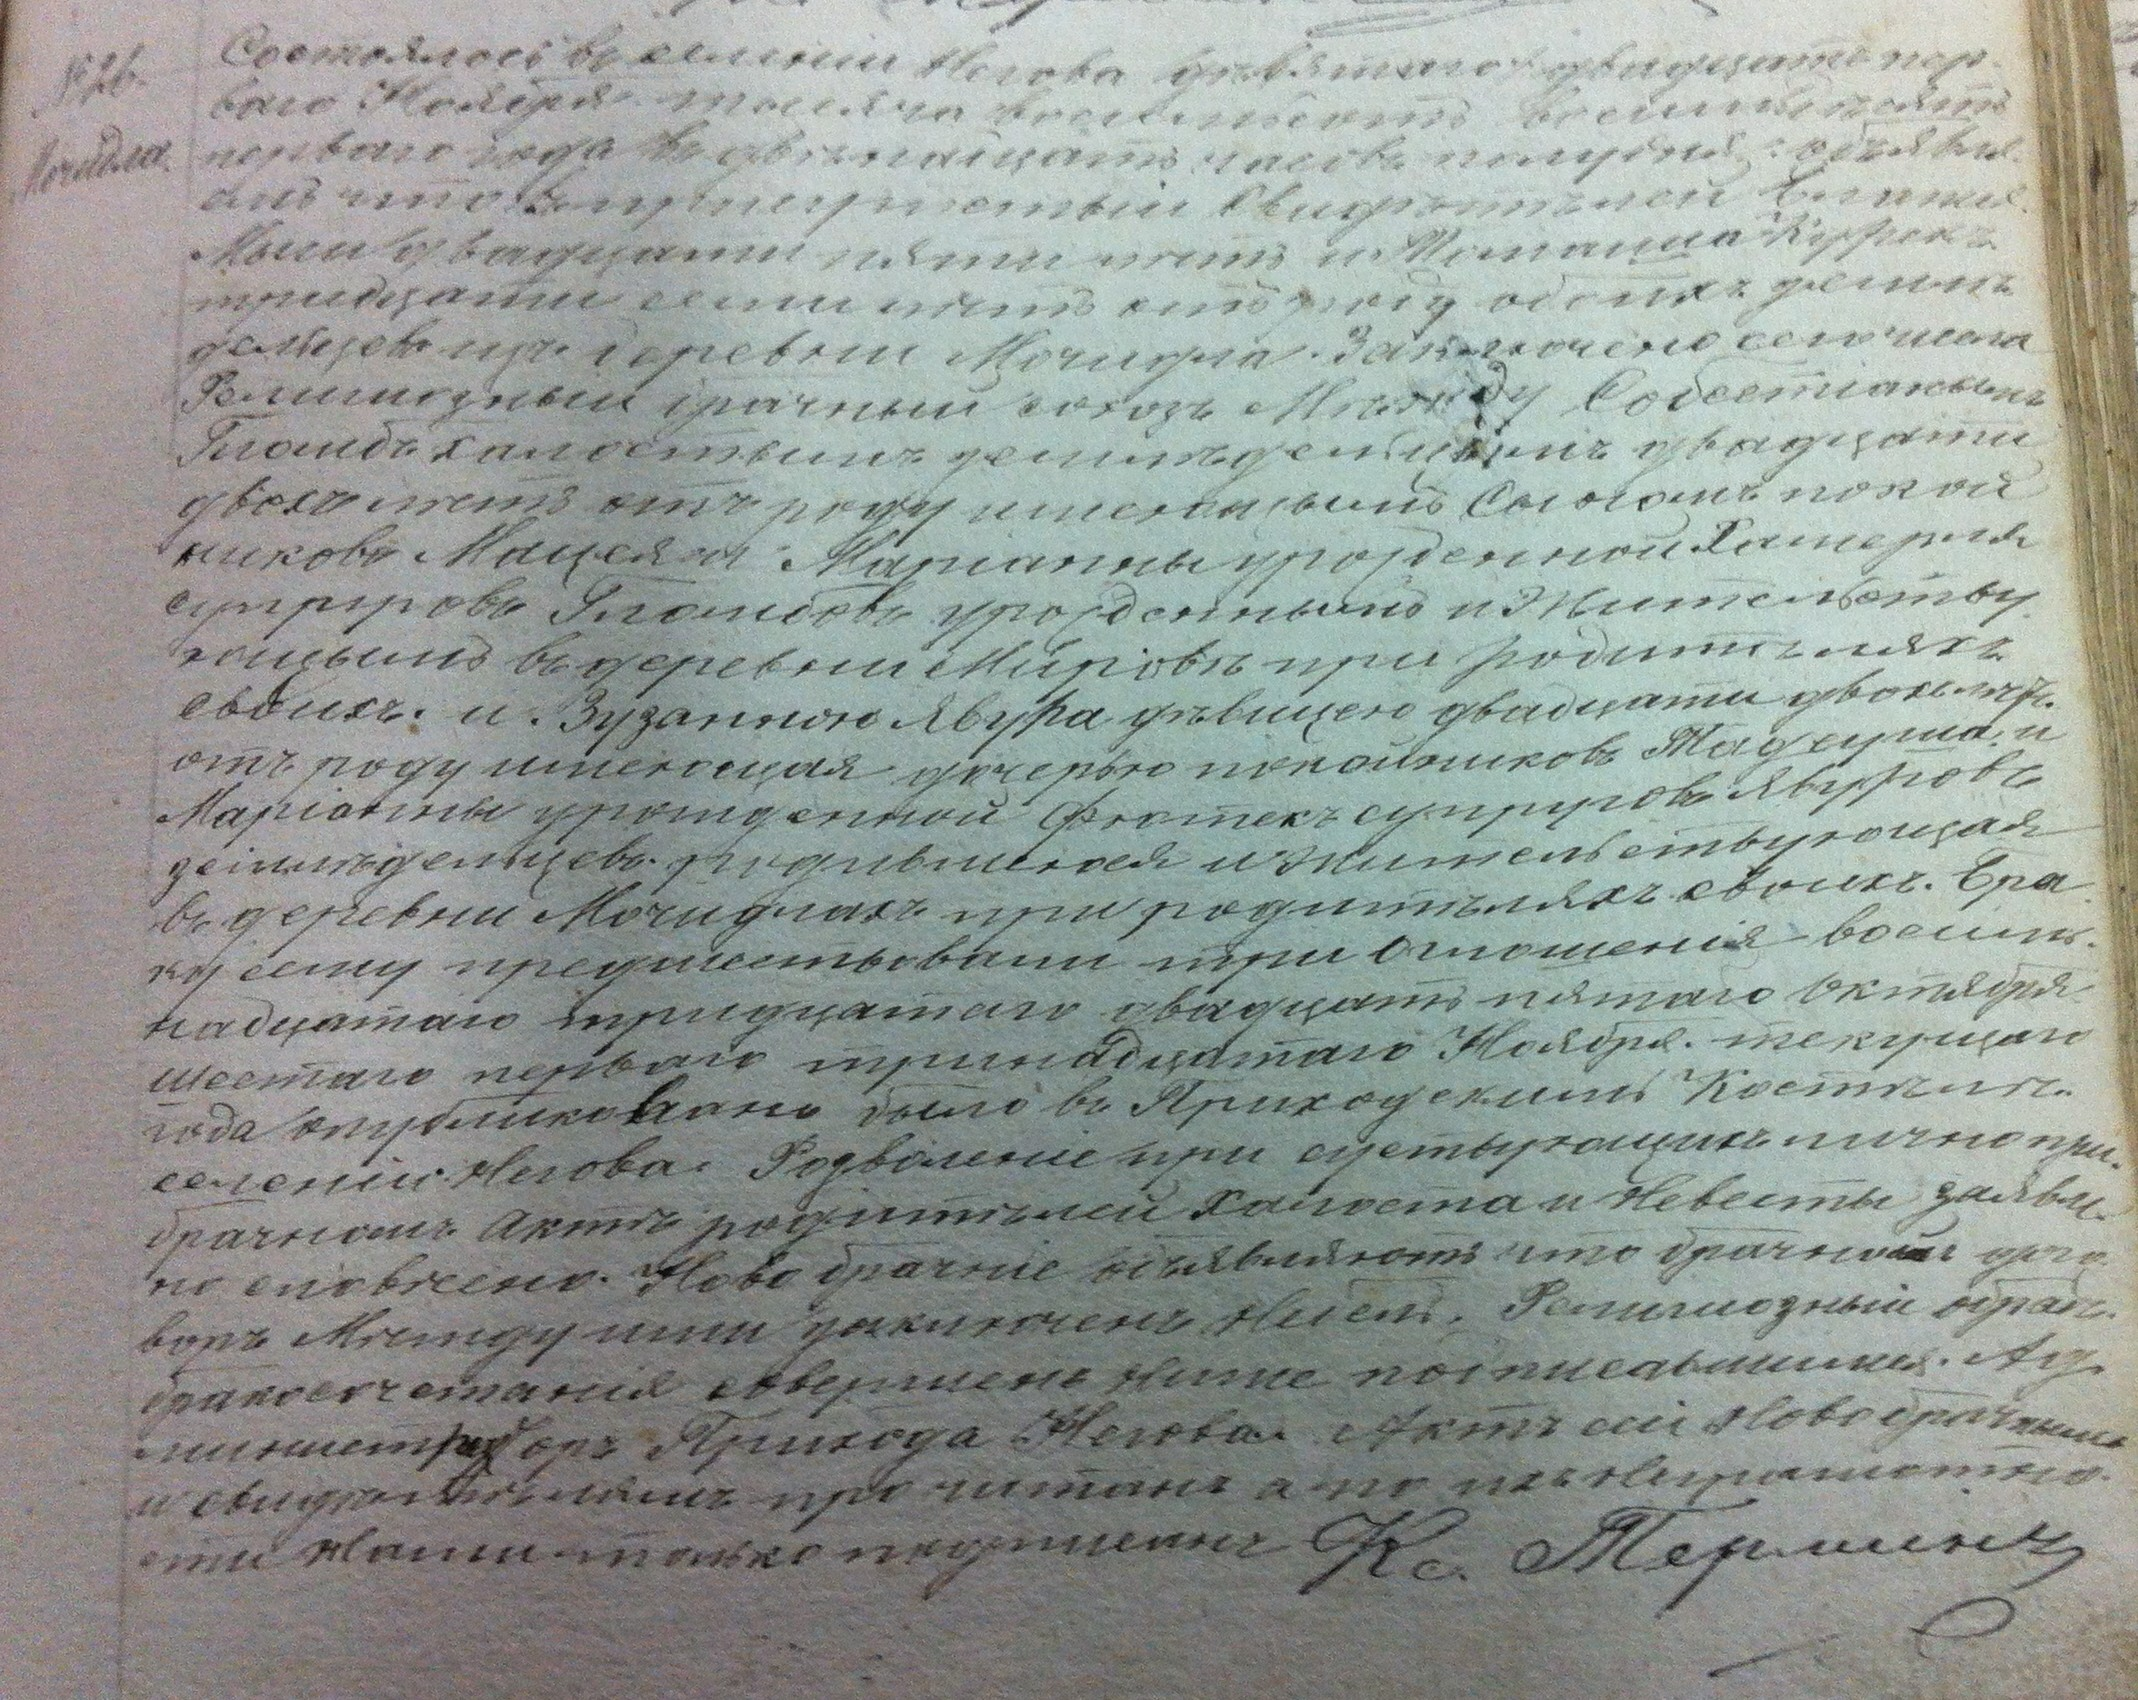
\includegraphics[width=0.7\textwidth]{zdjecia/akt_slubu_sobestiana_glaba_i_zuzanny_jawury.jpg}
\caption[Akt ślubu Sobestiana Głąba z Zuzanną Jawurą]{Akt ślubu Sobestiana Głąba (brata Walentego) z Zuzanną Jawurą}
\label{rys:akt_slubu_sobestiana_glaba_i_zuzanny_jawury}
\end{center}
\end{figure}

Po Sobosku, czyli Sobestyanie powinna się pojawić Antonina Głąb. Natomiast w 1861~r. pod datą 13 VII 1861~r. jest zapisany akt urodzenia i chrztu Marianny Głąb, córki Macieja i Marianny małżonków Głąbów. Rodzicami chrzestnymi byli Walenty Wasiak i Marianna Gurbała. Pod datą 27 VIII 1865~r. jest nawet odnotowany fakt urodzenia nieżywego dziecięcia Macieja i Marianny z Hamerlów małżonków Głąbów. Natomiast o Antoninie Głąb -- córce Macieja i Marianny Głąbów nie ma zapisu przed aktem urodzenia Walentego. Jest natomiast absolutnie pewne, że Antonina Głąb się niewątpliwie urodziła, wyszła za mąż i miała dzieci, lecz w księgach niegowskich jest taki zapis, ale dopiero po dacie urodzenia Walentego.

\begin{figure}[!h]
\begin{center}
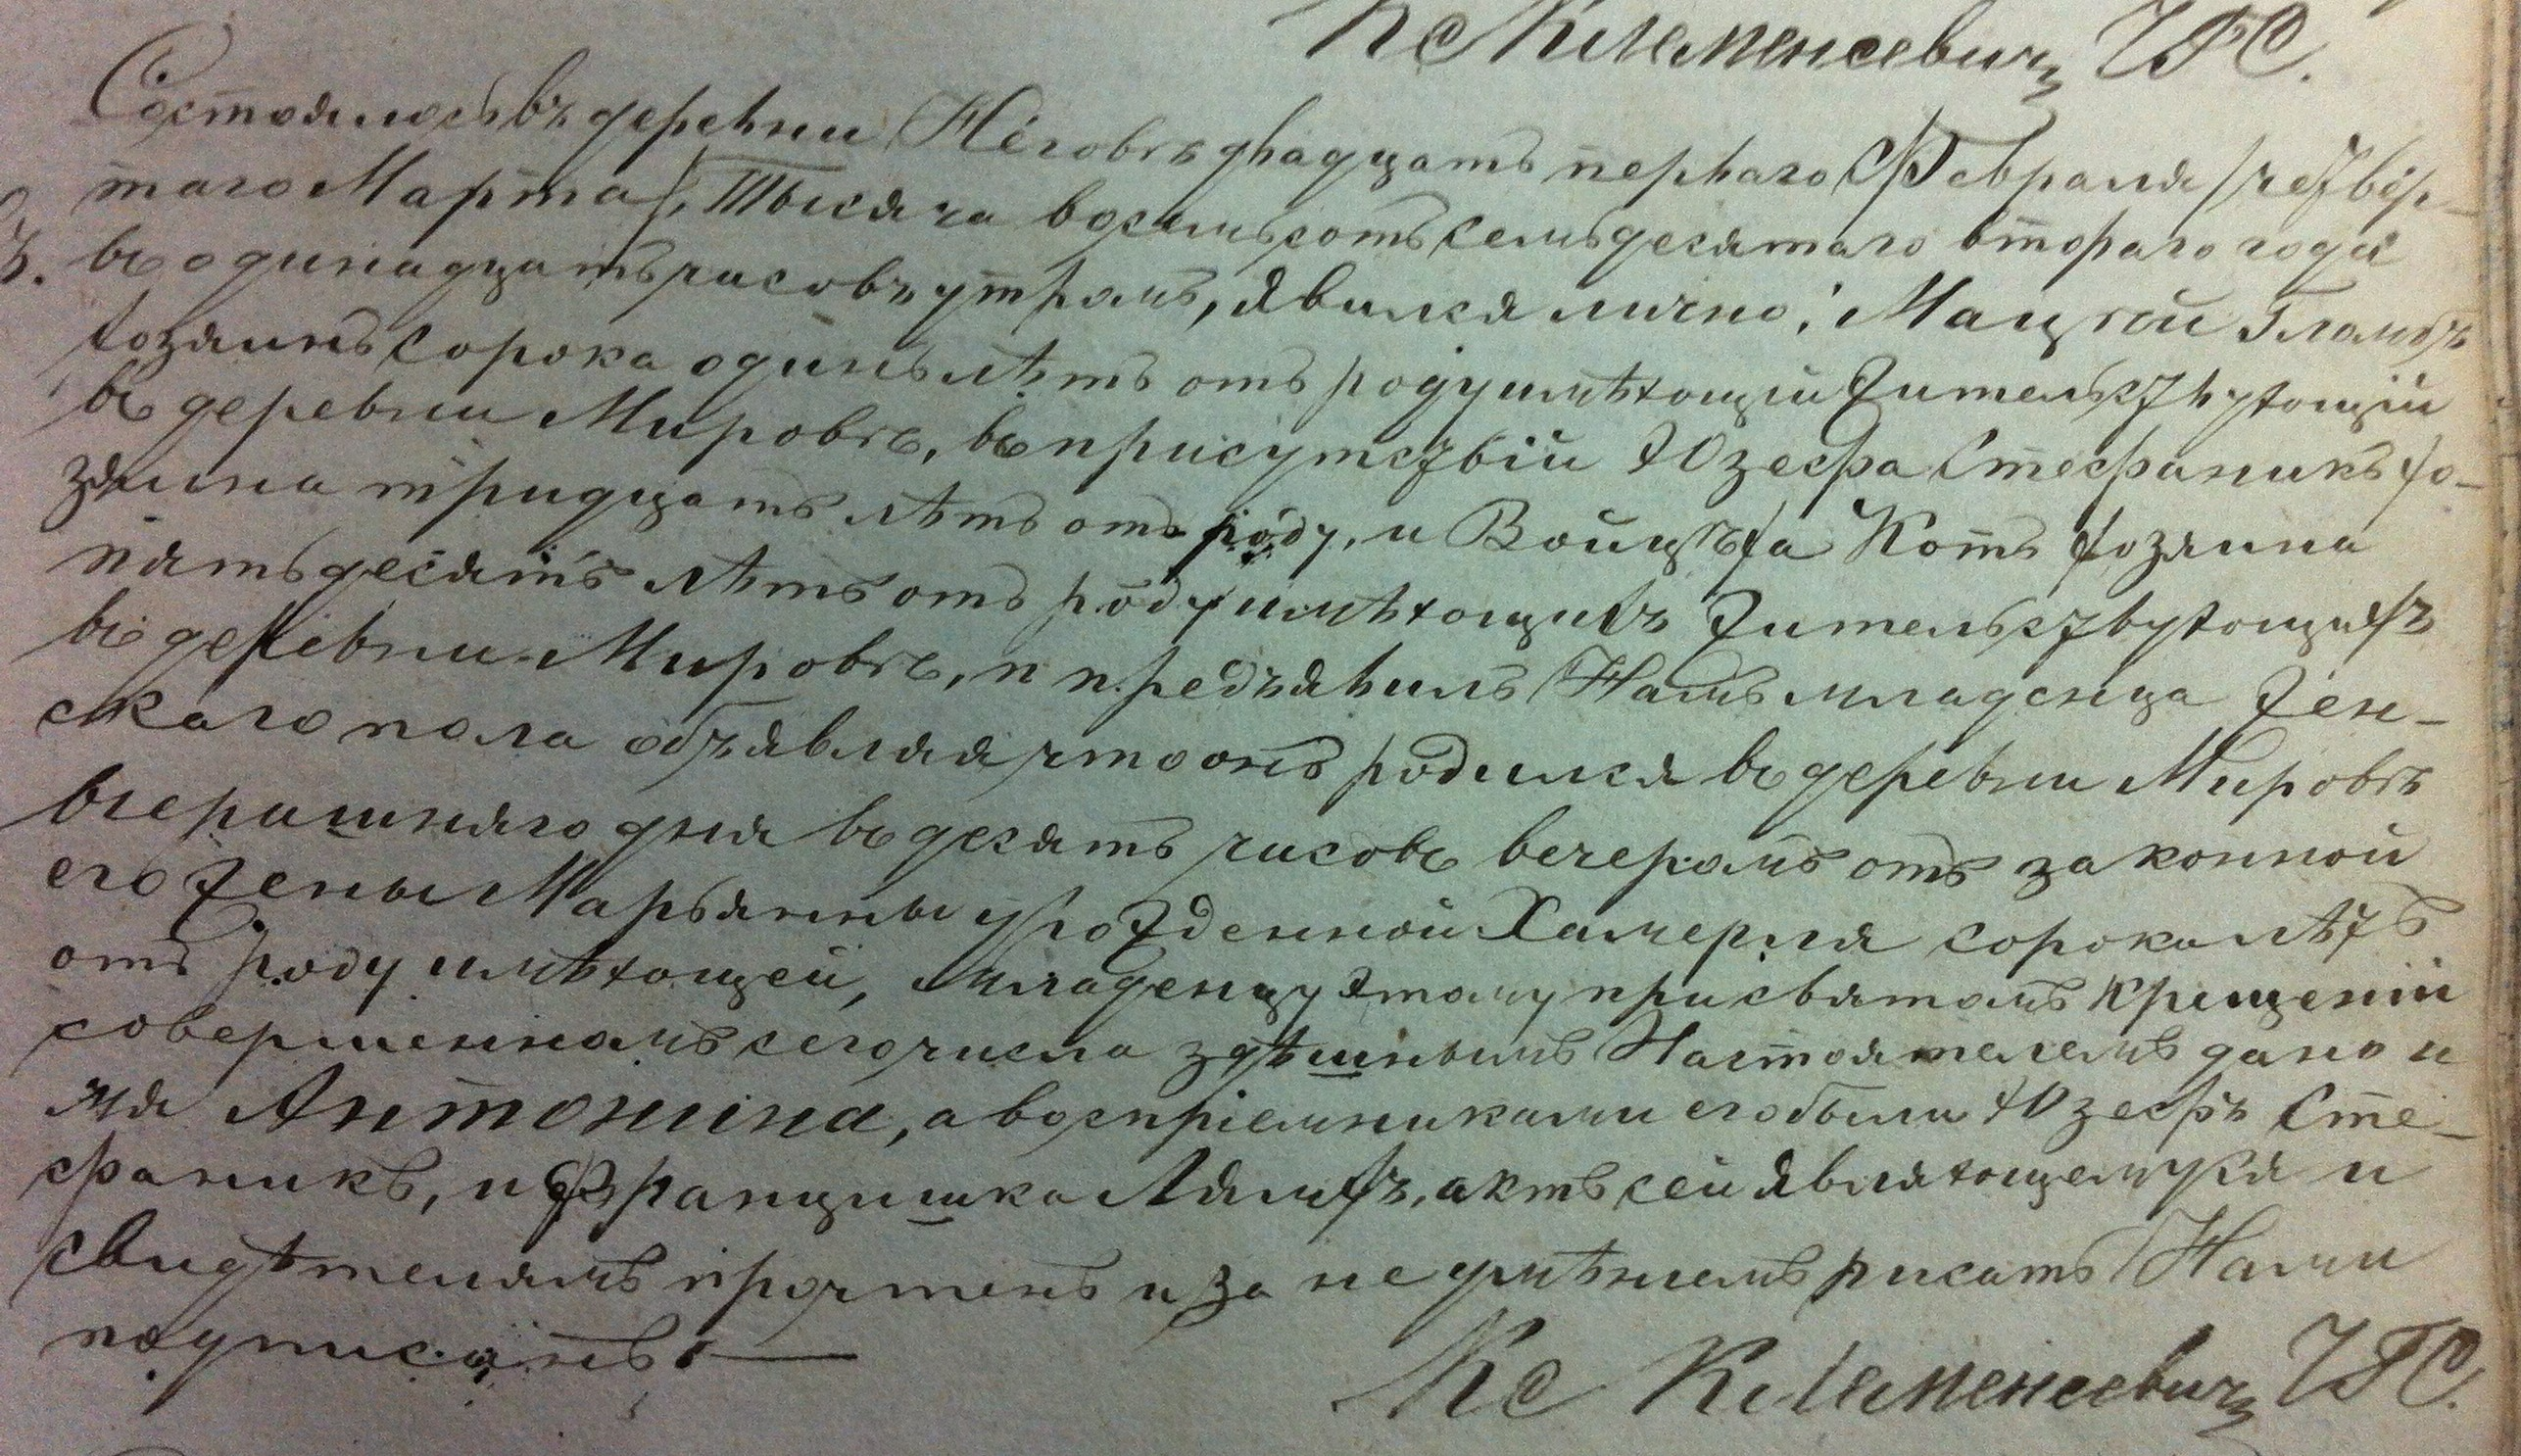
\includegraphics[width=0.8\textwidth]{zdjecia/akt_urodzenia_antoniny_glab.jpg}
\caption[Akt urodzenia Antoniny Głąb]{Akt urodzenia Antoniny Głąb -- córki Macieja i Marianny, a siostry Walentego}
\label{rys:akt_urodzenia_antoniny_glab}
\end{center}
\end{figure}

Oto 4 III 1872~r. stawił się Maciej Głąb gospodarz, lat 41, mieszkający we wsi Mirów, w obecności Józefa Stefanika, gospodarza, lat 30 i Wojciecha Kota, gospodarza, lat 50 -- mieszkańców wsi Mirów i okazał nam dziecię płci żeńskiej, które urodziło się dnia wczorajszego (tj. 3 III 1872~r.) w Mirowie o 10 wieczorem z jego prawowitej żony Marianny z domu Chamerla, lat 40. Dziecięciu temu nadano na chrzcie św. imię Antonina, a chrzestnymi byli Józef Stefanik i Franciszka Lamch. Chrztu udzielił ks. Klemensiewicz. (nr aktu 23).

\begin{figure}[!h]
\begin{center}
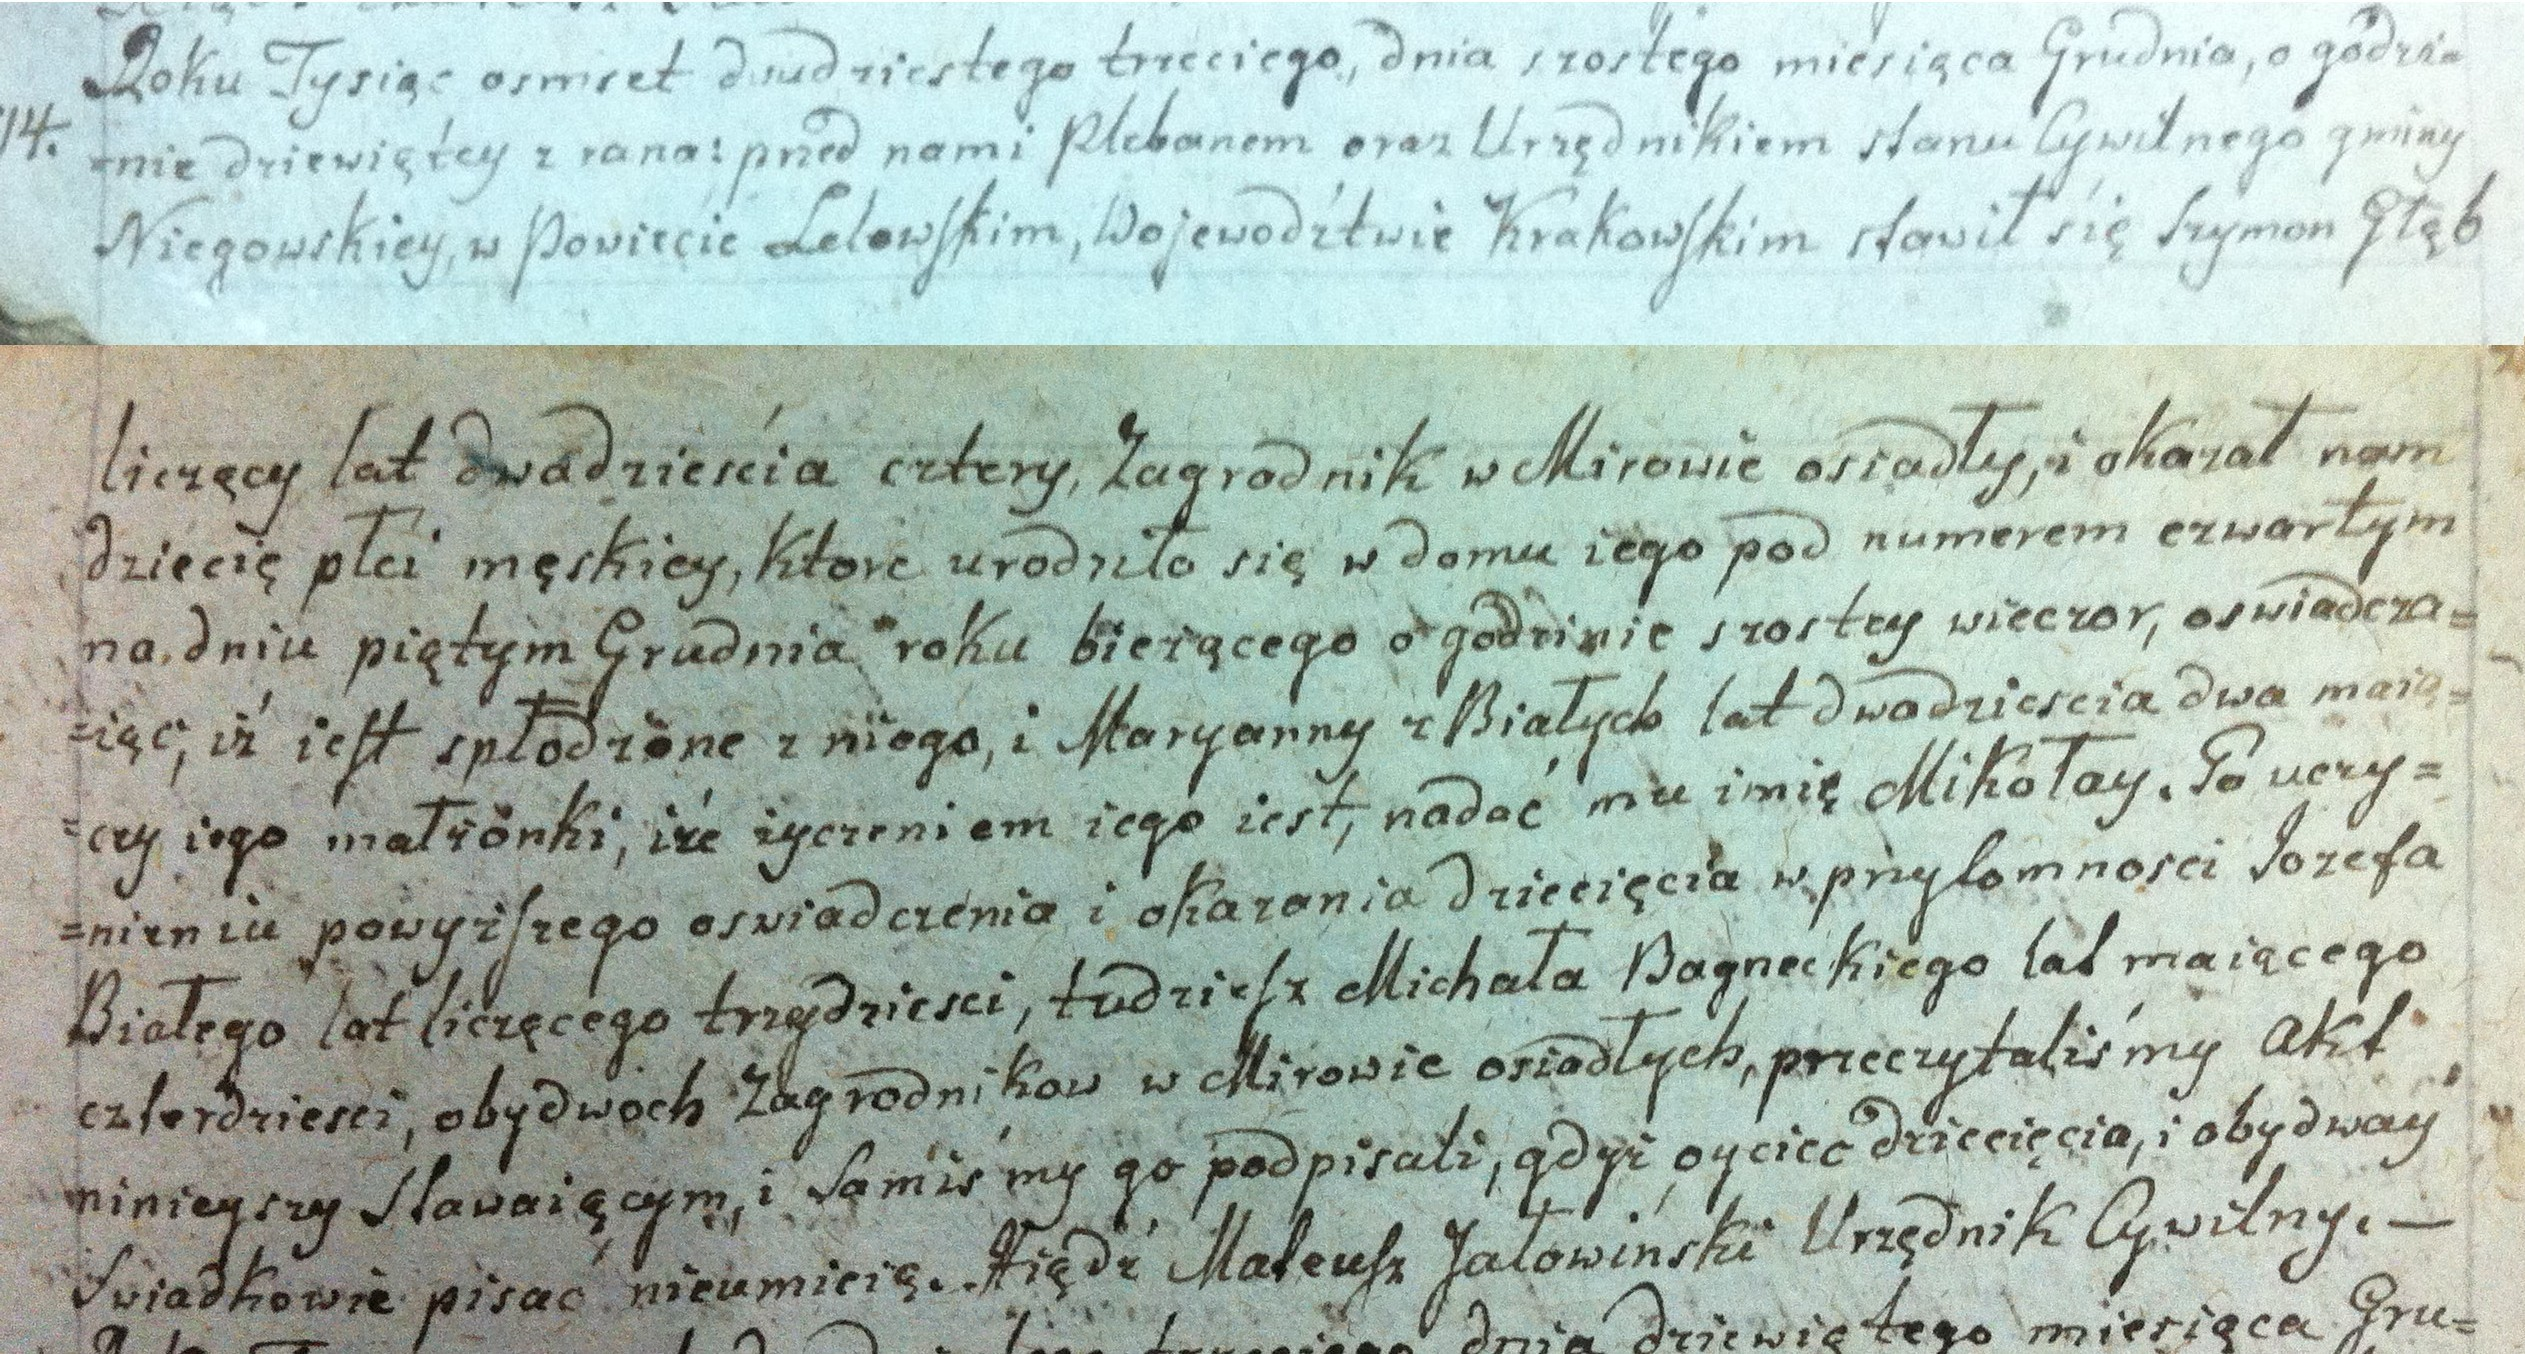
\includegraphics[width=0.8\textwidth]{zdjecia/akt_urodzenia_mikolaja_glaba.jpg}
\caption[Akt urodzenia Mikołaja Głąba]{Akt urodzenia Mikołaja Głąba -- syna Szymona i Marianny z domu Bialik, a brata Macieja}
\label{rys:akt_urodzenia_mikolaja_glaba}
\end{center}
\end{figure}

Maciej Głąb był szóstym dzieckiem Szymona Głąba i Marianny z Białów. Pierwszym ich dzieckiem był Mikołaj urodzony 5 XII 1823~r. w Mirowie. Wówczas Szymon -- jego ojciec miał 24 lata a matka Marianna miała 22 lata. A chrztu mu udzielał ks. Jełowiński. Po nim przyszły na świat 17 III 1826~r. bliźnięta Józef Głąb oraz Konstancja Głąbówna. W dwa lata później 12 V 1828r. przyszła Marianna Głąb, która pewnie niedługo żyła, skoro kolejne swe dziecko ochrzcili tym samym imieniem. 26 VII 1830~r. przyszedł na świat Jakub Głąb, który się ożenił i miał dzieci. 

Maciej Głąb przyszedł na świat 21 II 1833~r., a jego akt urodzenia wyżej cytujemy. Po nim 8 maja 1835~r. przyszła na świat Teresa Głąb, a w trzy lata później 25 VIII 1838~r. Marianna Głąbówna. Matką wyżej wymienionych dzieci w każdym akcie urodzenia i chrztu jest Marianna z Białych. Wcześniej, tj. przed Mikołajem nie zostało zapisane dziecko  małżonków Głąbów -- Szymona i Marianny z Białych. Można zatem przypuszczać, że Mikołaj był faktycznie ich pierwszym dzieckiem, a zatem najdalej w 1818~r. można szukać w księdze ślubów zapisu aktu ich małżeństwa.

I rzeczywiście w księdze ślubów parafii Niegowa znajdujemy obszerny opis tego zdarzenia, który w całości przytaczamy: ,,Roku 1822, dnia 14 stycznia przed nami Plebanem oraz Urzędnikiem cywilnym gminy Niegowskiej w powiecie Lelowskim, w  Województwie Krakowskim stawił się Szymon Głąb, młodzian ze wsi Kotowice parafii Włodowickiej, tamże służący, liczący według złożonej przed nami metryki wyjętej z ksiąg Kościoła Włodowickiego rok dwudziesty trzeci wieku swojego, syn zmarłego Franciszka Głąba zagrodnika w Kotowicach niegdyś osiadłego, którego śmierci dowiódł sepulturą z ksiąg Kościoła Włodowickiego wyjętą i przed nami złożoną i zmarłej jego małżonki Katarzyny z Zamorów Głąbowej, której śmierci dowodzi aktem zejścia z księgi aktów stanu cywilnego gminy Włodowice wyjętym i nam oddanym, niemający żadnego żyjącego z wstępnych, któryby aktowi małżeństwa jego assystował. Stawiła się także Maryanna Zębikówna, panna we wsi Mirów, parafii Niegowskiej urodzona, tamże przy rodzicach swoich zostająca, licząca według złożonej przed nami metryki z ksiąg Kościoła Niegowskiego wyjętej, rok dziewiętnasty wieku swojego, córka Tomasza Zębika  zagrodnika w Mirowie osiadłego i Marianny z Putaników jego małżonki w assystencji oboyga swoich rodziców: Tomasza i Marianny Zębików. Strony stawające żądają, abyśmy do ułożonego między nimi obchodu małżeństwa przystąpili, którego zapowiedzi w gminie naszej Niegowskiej ogłoszone zostały, tj. 30 XII 1821~r., 6 I 1822~r., tudzież w gminie Włodowickiej. Gdy o żadnym tamowaniu tak z gminy Niegowskiej jako i Włodowickiej rzeczonego małżeństwa uwiadomieni nie zostaliśmy, a rodzice niniejszym na obchód małżeństwa zezwalają i przychylając się zatem do żądania stron po przeczytaniu wszystkich wyżej wspomnianych papierów Działu szóstego Kodexu Cywilnego w Tytule o Małżeństwie, zapytaliśmy się przyszłego małżonka i przyszłej małżonki czyli chcą połączyć się z sobą związkiem małżeńskim?, na co, gdy każde z nich oddzielnie odpowiedziało, iż taka jest ich wola; ogłaszamy w imieniu prawa, iż Szymon Głąb i Marianna Zębikówna są połączeni z sobą węzłem małżeństwa. Czego akt spisaliśmy w przytomności Szymona Labochy, lat 39 liczącego i Tomasza Zamory mającego lat 28, wuja wyżej rzeczonego Szymona Głąba, a brata zmarłey matki jego, zagrodników we wsi Kotowice osiadłych, tudzież Tomasza Gurbały, lat 30 liczącego i Izydora Mygi lat 40 mającego obydwóch zagrodników we wsi Mirów osiadłych. Akt niniejszy został stawającym przeczytanym i od nas samych podpisanym, gdyż wszystkie wspomniane w nim osoby pisać nie umieją. Ksiądz Mateusz Jałowiński – Urzędnik Stanu Cywilnego.''

%TODO *** zdj. aktu ślubu Szymona Głąba z Marianną Zębikówną  nowy pdr. Nr 8 i 9. Ponieważ jest to fundamentalny akt ślubu rodu Głąbów postaraj się te stronice odpowiednio powiększyć, wyeksponować.
% Opis: Akt ślubu Szymona Głąba z Marianną Zębikówną -- dziadków (?) Walentego }

Wygląda na to,, że Szymon Głąb ożenił się z Marianną Zębikówną, a płodził dzieci z Marianną Białą (także Białową i Bialikową). Nad różnicą między Białą a Białową i Bialikową można byłoby przejść do porządku. Nierzadkie są przypadki słowotwórczego modyfikowania nazwisk włościan przez księży sporządzających owe zapisy. Natomiast różnica między Bialikówną a Zębikówną jest zasadnicza, co mnie skłoniło do powzięcia przypuszczenia, że w tamtym czasie było dwóch Szymonów Głąbów mieszkających w niegowskiej parafii. Podjąłem zatem poszukiwania aktu ślubu dla małżonków Szymona Głąba i Marianny Bialik lub Białej bądź Białowej. Przeszukałem zatem księgi parafii Włodowice, Żarki, Przybynów, Przyrów, Lelów oraz Irządze i nie znalazłem poza Niegową Szymona Głąba. Czyż w pańszczyźnianych czasach mógł chłop opuścić swego pana i ożenić się daleko od miejsca swego urodzenia? Skoro zatem po czasach napoleońskich było to już możliwe, to tym bardziej dręczyło pytanie: gdzie szukać? 

Tymczasem rozwiązanie (być może) tej tajemnicy przyszło dzięki Opatrzności Bożej ,,przypadkiem''. Oto coś mnie podkusiło, czego dotąd nie czyniłem, by ustalić datę zgonu Macieja Głąba oraz jego małżonki Marianny z Hamerlów.


%TODO *** Tu zdj. aktu zgonu Macieja Głąba; zdj. nr 185 w pliku Archiwum diecezj.
% Opis: Akt zgonu Macieja Głąba -- ojca Walentego }

Oto 19 III 1909~r. zmarł Maciej Głąb 81 lat (co nie w pełni jest prawdą, gdyż wg aktu urodzenia miał wówczas dopiero 76 lat, ale to nie pierwszy raz, że starzec dla większej estymy dodaje sobie lat) ,,syn Simiona Głomba i żieny jego Marianny urożdiennoj Bialik'' (w cudzysłowie podaję dokładną transliterację tekstu rosyjskiego), owdowiwszy żonę Mariannę Hamerlę mieszkającą we wsi Mirów.
W związku z powyższym postanowiłem się dowiedzieć ile lat przeżyła Macieja jego żona i odpowiedź znalazłem dopiero w księdze zgonów z 1920~r., oczywiście pisanej już po polsku.

%TODO *** Tu zdj. aktu zgonu Marianny Głąb, wdowy po Macieju; zdj. nr 187 w pliku Archiwum diecezj.
% Opis: Akt zgonu Marianny Głąb z domu Hamerla -- matki Walentego }

Oto ,,Dnia 12 XI 1920~r. stawili się Wojciech Lamch (56 lat) i Wojciech Kołacz (48 lat) włościanie ze wsi Niegowa i oświadczyli nam, iż we wsi Niegowa dnia 10 XI 1920~r. zmarła Marianna Głąb, \textbf{wdowa po zmarłym Macieju, synu Szymona i Marty z Zębików małżonków Głąb lat 94 licząca, córka Jana i Marianny z Czyżów małżonków Hamerla, urodzona w Ogorzelniku}, zamieszkała w Niegowie. (akt zgonu nr 114). Jeśli porównać dane osobowe Marianny Głąb z domu Hamerla, wdowy po Macieju Głąbie, to wszystko się zgadza co do joty. Istotnie była ona bowiem córką Jana Hamerli oraz Marianny z Cyzów.

Pod koniec życia dodawała sobie sporo lat, jako że faktycznie w chwili śmierci miała 84 lata, a nie 94, jak pewnie zapewniała tych, z którymi mieszkała i przestawała. I tak postępował niemal każdy wiekowy włościanin, gdyż przynajmniej za swój wiek był podziwiany, pozostając na łasce i niełasce swych dzieci lub nawet dalszej rodziny... Nasuwa się w przypadku Marianny Głąb z domu Hamerla ważkie pytanie: dlaczego mieszkała w Niegowie (a nie w Mirowie przy jednym lub drugim synu (przy Sebastianie lub Walentym) i u kogo? Przecież w chwili śmierci swego męża Macieja mieszkała w Mirowie, a w 11 lat później mieszkała i zmarła w Niegowie, wszystko bowiem wskazuje na to że ciągle mówimy o tej samej osobie, czyli żonie Macieja Głąba, syna Szymona Głąba i\ldots Marty z Zębików\ldots I tu mamy kolejne pytanie?! Przecież w akcie ślubu Szymona Głąba pojmuje on za żonę Maryannę Zębikównę, a nie Martę. Wiem z tradycji rodzinnej, że ostatnie lata życia Marianna, wdowa po Macieju Głąbie spędziła u córki w Niegowie. Owa córka miała na imię Antonina i w wieku 22 lat wyszła 28 stycznia 1896~r. w Niegowie za Józefa Lamcha -- kawalera lat 22, syna Michała i Franciszki z domu Fołtyn za mąż?

%TODO *** Tu zdj. aktu ślubu Józefa Lamcha z Antoniną Głąbówną; zdj. nr 293 w pliku Archiwum diecezj.
% Opis: Akt ślubu Józefa Lamcha z Antoniną Głąbówną -- siostrą Walentego }

Otóż istotnie Antonina Głąb 28 stycznia 1896~r. (a więc w dwa lata po swym bracie Walentym) wyszła za Józefa Lamcha – kawalera, lat 22 liczącego, syna Michała i Franciszki z Fołtynów w Tomiszowicach zamieszkałych. Antonina miała wówczas 22 lata (naprawdę miała wówczas 24 lata -- ur. 4 III 1872~r., ale ponieważ jej kawaler miał naprawdę 22 lata, więc ,,nie wypadało'', aby jego wybranka była od niego starsza) i była córką Macieja i Marianny z Chamerlów, zamieszkałą w Mirowie. Antonina urodziła się zatem w 1872~r., czyli trzy lata po Walentym (ryc.~\ref{rys:akt_urodzenia_antoniny_glab}).

U tej właśnie Antoniny znalazła Marianna Chamerla swoje przytulenie na ostatnie lata. A o jej zgonie świadczył nie przypadkiem Wojciech Lamch, skoro w domu Lamchów przyszło jej dokonać żywota. 
Przy okazji nie od rzeczy byłoby tu przytoczyć anegdotę krążącą w rodzinie Walentego Głąba, że Lamchowie w ramach umowy przedślubnej zażądali od Macieja wiana dla Antoniny w wysokości 2 kg złota, czyli złotej blaszki 10 x 10 cm o grubości 5 mm (tyle kosztowałyby owe dwa lata starszeństwa Antoniny wobec Józefa?).  Podobno wszystko to Lamchowie przepuścili, przepili, czego nie mógł odżałować Walenty i może stąd kwasy rodzinne, jakich Marianna Głąbowa po śmierci Macieja nie mogła znieść, więc się wyniosła do córki, którą tak kosztownie wywianowano. Grób Antoniny Lamchowej z Głąbów, która zmarła w 1951~r. oraz jej męża Józefa zmarłego w 1945~r. znajduje się na cmentarzu w Niegowie. Jest tam też pochowana Teresa Chłosta, z którą byliśmy w serdecznej przyjaźni (zmarła śmiercią samobójczą w stadium głębokiej depresji dnia 31 III 1998~r. w domu w Niegowie). Tam też leży jej matka Stanisława Królicka z domu Lamch, zmarła 31 V 1968~r. przeżywszy lat 54.

Odnosząc się do owych wątpliwości i nieścisłości stoję na stanowisku, że istotnie Szymon Głąb, ojciec Macieja Głąba, dziadka Franciszka Głąba, mojego teścia miał za żonę kobietę, która była różnie nazywana i też w  aktach metrykalnych, w akcie ślubu i w akcie zgonu różnie zapisywana: raz jako Marianna Zębikówna (w akcie ślubu z Szymonem Głąbem oraz akcie zgonu Marianny Maciejowej Głąbowej), drugi raz jako Marta Zębik wymieniona jako matka Macieja Głąba w akcie zgonu jej synowej – Marianny z Hamerlów Głąbowej, trzeci raz jako Marianna z Białych w akcie urodzenia jej pierwszego dziecka – Mikołaja Głąba, czwarty i piąty raz jako Marianna Bialikówna w akcie urodzenia bliźniąt: Józefa i Konstancji Głąbów, szósty raz jako Marianna z Białych w akcie urodzenia córki Heleny, siódmy i ósmy raz jako Marianna z Białów w akcie urodzenia syna Jakuba oraz syna Macieja... Cóż za nonszalancja wobec imion, nazwisk bądź to ze strony stawających bądź też spisujących akt... Tak czy owak nie mamy już świadków mogących rozstrzygnąć ostatecznie te nasze wątpliwości.

Przyjmujemy zatem, że najdawniejszym -- znanym nam antenatem rodziny Walentego i Antoniny z Łyszczarzów małżonków Głąbów jest Franciszek Głąb z Kotowic i jego żona Katarzyna z Zamorów -- rodziców Szymona Głąba. Skoro zatem w chwili ślubu z Marianną Zębikówną vel Bialikówną czy Białawą -- Szymon miał 23 lata, a żenił się w 1822 roku, więc prawdopodobnie urodził się w 1799 roku, a jego ojciec w latach 70’ XVIII wieku.

%TODO *** Tu zdj. aktu urodz. Marianny Zębikównej; zdj. nr 252 w pliku Archiwum diecezj.
% Opis: Akt urodzenia Marianny Zębikównej -- żony Szymona Głąba -- dziadka Walentego }

Marianna Zębikówna urodziła się 5 XII 1803~r. z ojca Tomasza i matki także Marianny (nazwiska jej nie podano, co w tamtych czasach było normą). Tak więc i jej rodzice urodzili się już w XVIII wieku. Jej rodzicami chrzestnymi byli Józef Gurbała i Elżbieta Balasowa. Cóż za dziwny zwyczaj, w akcie urodzenia podaje się imię i nazwisko rodziców chrzestnych, w tym także kobiety, a nie podaje się nazwiska matki biologicznej dziecięcia!

Akt urodzenia Marianny Zembik zaczyna się od daty: ,,5 Decembra 1803 idem baptisavit Mariannam hodie hora 8 matutina natan Laboriosorum Thoma Zembik e Mariannae Conjugum Legitt. Patrini fuere Josephus Gurbała et Elisabeth Balasowa des de Mirow.'' ( 5 grudnia 1803 tamże ochrzciłem Mariannę, tego dnia o godzinie 8 rano urodzoną, spłodzoną przez Tomasza Zembika i Mariannę prawowitych małżonków. Rodzicami chrzestnymi byli Józef Gurbała i Elżbieta Balasowa, oboje z Mirowa.)

Rodzicami owej Marianny Hamerli (czasami pisanej jako Chamerla lub Hamerlikowa) byli Jan Chamerla ur. 6 lutego 1787~r. w Ogorzelniku z ojca Benedykta bądź Bonawentury i matki Heleny (Haliny) z Bednarczyków oraz Marcyanna z Cyzów Chamerla ur. 25 XII 1808~r. w Kotowicach z ojca Kazimierza i Zofii z Gurbałów. Jej rodzice pobrali się 25 lutego 1827~r. we Włodowicach. Było to drugie małżeństwo Jana Chamerli po śmierci jego pierwszej żony -- Magdaleny Wasiak zmarłej 4 II 1827~r.

%TODO *** Tu zdj. aktu urodz. Jana Hamerli; zdj. nr 289 w pliku Archiwum diecezj.
% Opis: Akt urodzenia Jana Hamerli -- dziadka Walentego ze strony matki }

Wypada jeszcze dodać urodzenia dzieci -- braci Macieja Głąba oraz brata Walentego Głąba w ten sposób potwierdzając, że dożyli wieku dojrzałego (w tamtych czasach śmiertelność niemowląt była bardzo wysoka). Wymieniam je, przypisując do poszczególnych ojców: Jakub Głąb, syn Szymona Głąba, ur. 26 VII 1830~r. spłodził z Marianną z Kurków w Mirowie: 1. Józefę Głąb ur. 15 III 1863~r., 2. Mariannę Głąb ur. 11 IX 1868~r., 3. Pawła Głąba ur. 19 I 1871~r., 4. Ewę Głąb ur. 20 VII 1874~r., 5. Błażeja Głąba ur. 1 II 1878~r.

Dzieci Sebastiana Głąba (ur. w 1859~r., brata Walentego) i Zuzanny z Jawurów ur. w Mirowie: 1. Andrzej Głąb ur. 8 XI 1882~r., 2. Jan Głąb ur. 29 X 1885~r. 3. Antonina Głąb ur. 30 V 1888~r., 4. Marianna Głąb ur. 11 VIII 1894~r., 5. Franciszek Salezy Głąb ur. w 1897~r., 6. Józef Głąb ur. 27 X 1899~r. jak wszyscy poprzedni w Mirowie.

\begin{figure}[!h]
\begin{center}
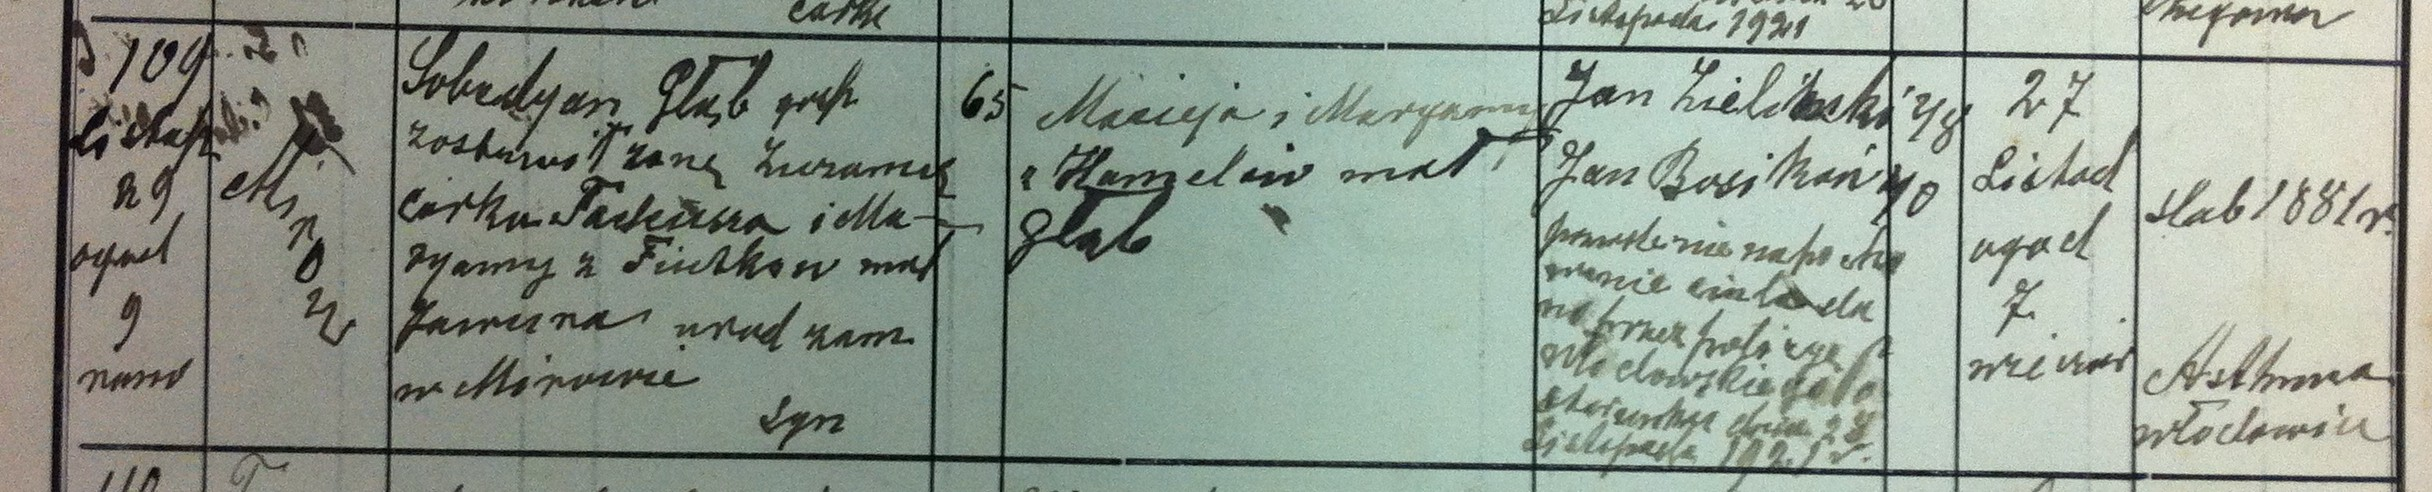
\includegraphics[width=0.8\textwidth]{zdjecia/akt_zgonu_sobestiana_glaba.jpg}
\caption[Akt zgonu Sobestiana Głąba]{Akt zgonu Sobestiana Głąba -- brata Walentego}
\label{rys:akt_zgonu_sobestiana_glaba}
\end{center}
\end{figure}

Franciszek Głąb -- syn Sebastiana - kawaler - zmarł 24 IX 1921~r. Musiał to być straszny cios dla ojca, skoro w dwa miesiące później, tj. 27 XI 1921~r. zmarł w wieku 65 lat (wedle zwyczaju doliczył sobie cztery lata), syn Macieja i Marianny z Hamerlów, włościanin, który zostawił żonę Zuzannę, córkę Tadeusza Jawury i Marianny z Fiutków.

Wypada, idąc tropem przywołanego wyżej porzekadła o malowanych dzieciach, dodać jeszcze spis dzieci Antoniny Głąbianki i Józefa Lamcha: 1. Stanisław Lamch ur. 2 VII 1897~r., 2. Franciszek Lamch ur. 13 IV 1899~r., 3. Marcin Lamch ur. 16 XI 1900~r., 4. Olimpia Lamch ur. 11 VIII 1908~r. oraz 5. Stanisława Lamch ur. w 1914 roku (wspomniana wcześniej matka Teresy Chłosty), wszyscy urodzeni w Tomiszowicach.

Tak oto przedstawia się historia rodziny Walentego i Antoniny Głąbów. Jest w niej trochę białych plam zwłaszcza w najnowszej historii a to z powodu niechęci niektórych członków tej nad wyraz płodnej rodziny do przekazania informacji o datach urodzenia ich rodzeństwa bądź potomstwa a także daty ich ślubu. Białe plamy w głębokiej przeszłości usprawiedliwia przede wszystkim brak ksiąg (zwłaszcza w parafii włodowickiej brak ksiąg z wieku XVIII. Księgi metrykalne parafii niegowskiej sięgają połowy XVII w.
Nie każda też rodzina została zilustrowana zdjęciem, gdyż takowego nie była chętna przekazać. A przecież mało który z rodów może się poszczycić posiadaniem historii sięgającej XVIII w. 

Pamięć rodowodu wyróżnia człowieka od zwierząt. Ba! Wyróżnia szlachtę od prostactwa. Rzeczownik szlachta wywodzi się od niemieckiego słowa geschlecht, które oznacza rodowód. Szlachcicem mógł być ten, który potrafił wywieść swój rodowód od dziada, pradziada... Co więc powiedzieć o kimś, komu podaje się jakby na tacy jego rodowód, a on tym gardzi... Wiadomo, koryta tym nie napełni, bo na co mu to się zda! Nie przejmujmy się nimi i szlachetniejmy bogactwem swych rodowodów... Godzi się natomiast w tym miejscu gorąco podziękować Marcinowi Skowronkowi -- praprawnukowi Walentego i Antoniny Głąbów, który wiele trudu włożył w to, by wszystkie zdjęcia rodziny oraz aktów metrykalnych zostały zeskanowane, a także Bożydarowi Świerczyńskiemu -- prawnukowi wyżej wymienionych antenatów za trud umieszczenia owych skanów we wskazanych miejscach tekstu i wreszcie dzięki Mirosławowi Głąbowi -- za wszelką pomoc oraz okazywane zainteresowanie postępami prac w dziele odkrywania rodowych tajemnic.

Nasze (\textbf{dzieci Franciszka Głąba}) korzenie przedstawiają się następująco: 
\begin{itemize}
\item dziadkami naszymi ze strony ojca są: \textbf{Walenty i Antonina z domu Łyszczarz Głąbowie}, 
\item pradziadkami: \textbf{Maciej i Marianna z domu Hamerla Głąbowie} (rodzice Walentego) oraz \textbf{Maciej i Józefa z domu Boniek Łyszczarzowie} (rodzice Antoniny),
\item prapradziadkami: \textbf{Szymon i Marianna z domu Bialik (najprawdopodobniej Zębikówna) Głąbowie} (rodzice Macieja), \textbf{Jan i Marcjanna z domu Czyż (Cyz) Hamerlowie} (rodzice Marianny), następnie \textbf{Bartłomiej i Ewa z domu Filipecka Łyszczarzowie} (rodzice Macieja), \textbf{Paweł i Zofia z domu Juszczyk Bońkowie} (rodzice Józefy),
\item praprapradziadkami: \textbf{Franciszek i Katarzyna z domu Zamora Głąbowie} (rodzice Szymona), nieznani są rodzice Marianny Bialik, \textbf{Benedykt i Helena z domu Bednarczyk Hamerlowie} (rodzice Jana), \textbf{Kazimierz i Zofia z domu Gurbała Cyzowie} (rodzice Marcjanny), nieznani są rodzice Bartłomieja Łyszczarza ani też Ewy Filipeckiej, \textbf{Kazimierz i Agnieszka z domu Piasecka Bońkowie} (rodzice Pawła) oraz \textbf{Idzi i Elżbieta z domu Wcisło Juszczykowscy} (rodzice Zofii)
\end{itemize}


Niniejszą historię spisał Czesław Świerczyński, 
mąż córki Franciszka Głąba z Mirowa 
a także prapraprawnuczki Franciszka Głąba z Kotowic.




